\documentclass[12pt]{article}
\usepackage{booktabs,simplemargins}
\usepackage[sort&compress]{natbib}
\usepackage{amsmath,amsfonts,latexsym,amssymb,amsbsy}
\usepackage{color}
\usepackage[colorlinks=true,citecolor=cyan,linkcolor=blue,urlcolor=magenta]{hyperref}
\usepackage{subfigure}
\usepackage{tabularx}
% select graphic handling: different for Mac v. PC

\usepackage[pdftex]{graphicx}
\usepackage{epstopdf}



% define margins
\setallmargins{1in} 

\title{A framework to detect vaccine related misinformation using social media data}
\author{Muhammad Farhan Riaz, Matthew Vassov, Neha Basra \\ Melodie Y. Song\thanks{CIHR Health Systems Impact Fellow, Equitable AI for Public Health at Public Health Ontario {\tt melodie.song@oahpp.ca}} , Dionne M. Aleman\thanks{Department of Mechanical and Industrial Engineering, University of Toronto; 5 King's College Road, Toronto, ON M5S 3G8, Canada; {\tt aleman@mie.utoronto.ca}}}

\date{\today}





\begin{document}

\maketitle



\begin{abstract}
As social media, namely Twitter, has become an active source for Public Health surveillance research, there is a need for an easily followed framework which allows for a robust and convenient way for researchers to deploy a model and a Tableau based dashboard to get a \textit{pulse check} for Public Health related concerns. The dashboard allows for slicing of data in different ways (by geography, user, most-retweeted Tweets etc.). This project introduces this framework and dashboard by showcasing its application on a set of Twitter data (including full text of the Tweets and web-scraped URLs within them) to detect Vaccine related misinformation leading up to the onset of the COVID-19 global pandemic.

The framework trains 9 different classifiers on randomly under-sampled annotated data which are compared against 5 distinct class categorizations (ranging from five classes to three classes), trained using 7-fold cross validation paired with a grid search method evaluating the best hyper-parameters for each classifier. While 7,987 Tweets were annotated for this application, the under-sampled training sample was almost 5,000 Tweets. 

Final selected model for this application was a four class categorization with a Logistic Regression Classifier, achieving a Macro F1 Score of 0.502 and Accuracy of 0.504 on randomly under-sampled data. The results from non-sampled data are also provided for comparison, which provided an accuracy as high as 0.686 in a three class categorization and 0.604 in a five class categorization but significantly poorer F1 scores due to the imbalanced dataset with one class (positive sentiment) dominating the training examples over the remainder classes (the neutral and misinformation classes). It should be noted that significant content drift was observed in the data.


\end{abstract}

\newpage

\tableofcontents




\newpage






\section{Introduction} \label{sec:intro}

Social media represents a source of knowledge and insight from the perspective of the individual posting the material. Users and followers alike can share mass amounts of information at the simple click of a button. Issues may arise however, when the information being shared is intentionally false, or doesn’t speak to the whole truth.  One of the unforgiving properties of false information is that it tends to evoke emotions of anger and surprise, which associates with these information travelling further, deeper, and wider on social media \cite{vosoughi-2018}. Amidst the COVID-19 pandemic in 2020, the spread of viral false information has led to real-life public health ramifications – from alcohol poisoning in Iran, chloroquine poisoning in Nigeria, and roughly 5800 known deaths associated with misinformation of COVID-19 treatment and cure in 87 countries \cite{islam-2020}.   


More worrisome are anticipated vaccine-preventable disease outbreaks associated with a decrease in immunization coverage during the pandemic due to stay-at-home orders and resource allocation for pandemic relief around the globe. Heralded as the top 10 public health inventions of the 20th century by the World Health Organization, immunization programs are fundamental to preventing the spread of vaccine-preventable diseases; they boost immunity, protect people from dangerous diseases, and ultimately prolong lifespan. Despite its benefits, social media is rife with polarising distrust towards vaccinations amidst the COVID-19 pandemic. Efforts to promote vaccine awareness are circumvented by those with ulterior motives to misinform the public , and proliferated by the public whose conspiratorial thinking and mistrust in conventional Western medicine \cite{hornsey-harris-2018,hornsey-lobera-2020}. 

When people post untrue vaccination claims over social media, their falsified information may influence groups of people from protecting themselves or their loved ones.  As such, the spread of this information cost lives and poses a burden on the global health care system. The WHO has estimated that coverage of essential vaccinations for children and adolescent may reduce from an average of 70\% to less than 50\% in 2021, adding a steep decline to an already slow decline in vaccination coverage over the last decade due to vaccine hesitancy \cite{WHO-top10-2020} . 


The purpose of this project is to analyze a large Twitter database and use natural-language-processing (NLP) in unison with different machine learning models to make predictions about whether a tweet is spreading misinformation or not. 

A secondary purpose of this project is to provide a framework for quickly training and deploying a machine learning model for a similar topic using similar data sources in order to cut down time for future analyses and add additional value to decision makers. The code files supplementing this report are intended to be mostly ‘plug and play’, further allowing additional value with code that can be used for data pre-processing, web scraping and model training \& comparison. Good knowledge of Python and basic understanding of machine learning concepts is expected to fully utilize this framework.  



\section{Literature Review}
\subsection{Data Analysis \& Reasoning}
Vaccination hesitancy is considered the top 10 threats to global health in 2019 \cite{WHO-top10-2019}. The Vaccine Confidence Project estimates that globally, anywhere around 13\%-40\% of the population based on a 67-country survey are vaccine hesitant \cite{larson-2016}. From a medical anthropological perspective, vaccine hesitancy is highly contextual: sensitive to historical, sociopolitical, and economic conditions, the reasons people refuse vaccination demonstrates temporal and spatial dynamism unique to a targeted vaccine or a spectrum of vaccines \cite{dube-gagnon-2014, dube-vivion-2015}.  

While large-scale surveys are useful in understanding the prevalence of vaccine hesitancy, limitations abound as surveys are costly and time-consuming. To overcome this limitation, researchers over the last 5 years have turned to Natural Language Processing, a “subfield of Artificial Intelligence that is devoted to developing algorithms and building models capable of using language in the same way humans do” \cite{balic-2020}. Often an interdisciplinary process require the expertise of content experts in public health and data science, NLP is increasingly explored as a way to disentangle vaccine sentiment on social media, particularly when processing unstructured free-text. A bourgeoning field of research in public health, NLP can help us determine the linguistic, psychosocial, and emotional properties that correlate with misinformation spread \cite{monsted-2019}.

In 2019, Du et al classified 652,252 English tweets collected between 2013-2017 on Human Papillomavirus (HPV) vaccines by 4 health belief constructs (i.e., perceived susceptibility, perceived severity, perceived benefits, and perceived barriers), They used a recurrent neural network (RNN)-based deep-learning framework to classify unannotated tweets, achieving 80.50\% accuracy on overall classification and between 80.33\%-89.82\% accuracy or the four health belief constructs.   

In 2018, Elenora D’Andrea et al. studied the topic of public opinion about the vaccination topic from tweets in Italy. Using a three-class system for text classification (in favor, not in favor and neutral), adopting a bag-of-words approach with stemmed n -grams as tokens, and the support vector machine (SVM) model for classification – the team was able to produce a system to provide real time monitoring of public opinion about vaccine decision making. \cite{elenora-etal-2018}

In 2019, Bjarke Mønsted and Sune Lehmann studied vaccine discourse using data collected from Twitter within an online system.  They trained a deep neural network on a two-class target vector, producing an accuracy of 90.4\%, and an F1-Score of 76.2\% on a three-class target vector.  Their data primarily consisted of user accounts who were either extremely anti or pro-vaccine (with little variation in-between) \cite{monsted-2019}.  Originally, 10,000 tweets were labelled among 3 hired annotators.  This number was reduced to 5,358 based on their mutual agreement on the tweet sentiment (ie. tie-breaking).  From there, 10,670,000 further tweets were downloaded based on the hashtags of the original 5,358.  This massive database of tweets was then used to train their deep neural network model.

While the intent for this project is to look at a five-class system (i.e., pro-, neutral, irrelevant, and two classes of anti-), utilizing a bag-of-words vectorizer, stemming n-grams as tokens and implementing an SVM model will be explored as per D’Andrea et al’s approach. Additionally, just as Mønsted and Lehmann have done, tweet annotations will be tie-broken by a third party and ultimately trained on a deep neural network.




\subsection{Under \& Oversampling}
Problems may arise in any model if there is a severe imbalance of data; that is to say, the counts of each target label are not distributed equally. In situations like this, it is possible and very likely that the machine learning model may form a bias towards classes that contain more labels than others.  While the ultimate goal of this project is to distribute the number of class labels evenly, to have expectations for this may prove to be unrealistic, and so other strategies such as guided undersampling and oversampling must be taken into consideration.  

In 2018, W. Eric Brown et al. applied different model classification techniques on an imbalanced dataset pertaining to automated radiation therapy quality assurance process on prostate cancer treatment. Such techniques to overcome class imbalances of minority data included the use of SVM’s, decision trees and neural networks.  Perhaps the most impactful approach however, was to use guided undersampling, the strategical implementation of which can be credited to Sung et al.  This method, which applies both advanced filtering techniques and various data classification strategies, resulted in significant performance gains \cite{brown-etall-2018}.

According to W. Eric Brown et al., guided undersampling is a widely used classification technique that addresses the issues of imbalanced data \cite{brown-etall-2018}. Theoretically, for the scope of this project, if this technique is applied to classes that have an overabundance of labels, guided or random under-sampling can be applied to the surplus classes.  Alternatively, the classes that have smaller label counts can be oversampled by duplicating the number labels being fed to the machine learning model.  


The ultimate goal of this project is to have 2,500 labeled annotations per class, which in theory, should be sufficient to train each classifier on. This would result in approximately 12,500 total sample annotations.  If this goal is reached, there may be no reason to implement over and under-sampling.  Alternatively, if the goal cannot be reached and there is a large target-label imbalance, both techniques will be explored.

\subsection{Social Media Web Scraping}

This project primarily uses the Twython API to extract the data needed for NLP analysis and machine learning.  In the data preprocessing workflow, the Twitter ID’s are provided and run through the API in order to extract information such as the tweet, the user, their location, the date, etc. After the data has been cleaned using various NLP tactics, the output is a “cleaned” version of the original tweet; meaningless words and characters have been removed, words have been tokenized, and the original word has been replaced with its root.  Problems arise however, when the resulting cleaned text is left as a “blank”.  This is due to the possibility of all words within the tweet being meaningless.  To further complicate this, most retweets where the user is responding to another tweet by incorporating the URL result in a blank clean text.  In order to properly understand what was originally said in the “blank” tweets, the contents of the URL must be decrypted and analyzed to correctly classify the sentiment of these tweets. 


Web scraping is an important part of data extraction that can be used for a multitude of reasons.  Glez-Pena et al. describe web scraping as the process of extracting website content using a systematic approach. They state that web services are a standard for biomedical data interoperability and as such, much be utilized for when programmatic interfaces or API’s are insufficient in extracting the tools/ data required \cite{glez-pena-etal-2013}.  While this article focuses on scraping for bioinformatics related data, the same concept can be applied within this context.  After initially exploring the data, it was found that approximately 22\% of tweets from the consolidated database contained a URL in reference to another post, article, or news segment.  The opinion of each URL source will ultimately affect the opinion of the tweet and should therefore not be discredited.


To effectively gather the URL web content,BeautifulSoup(v. 4.9.0) \cite{crummy-2020}, an open-source Python module isused to extract headers, titles and paragraphs from the webpages. Each of the three are tested, with the most effective being implemented in the final data preprocessing script.   



\subsection{Grid Search \& K-Fold Cross Validation}
In machine learning, each model must be trained before being fully implemented on the dataset.  This will allow for an analysis performed on the accuracy and other desired evaluation metrics, which will be discussed later.  According to Yoonsuh Jung and Jianhua Hu, cross validation is a widely accepted method of training models in the machine learning world.  K-fold cross validation is the process of splitting the dataset evenly and randomly into “K” parts (K = 7 for this project), which act as the model’s training set \cite{jung-2014}.  By approaching the problem in this fashion, this will allow for diversity in training; the model will be exposed to different sets of data and will average the test results based on the different evaluation metrics.
While cross validation is the ideal approach for this project, a quick and efficient way to gather the optimal results is also required.  As such, using a grid search will be explored.  Grid search is the process of running multiple classifiers with different hyperparameters through an optimizer that outputs the classifier(s) and hyperparameters with the best performance. Piehowski et al. utilized a grid search methodology for optimized peptide identification filtering which is a powerful data analysis tool with a focus in optimal filtering patterns and quality control \cite{piehowski-etal-2013}.  Since there is potential in utilizing multiple classifiers, vectorizers and hyperparameters, it makes sense to run all iterations of these through a grid search to increase efficiency.



\section{Data Acquisition}

\subsection{The dataset}
The dataset for this project and modeling was sourced from Twitter. The dataset is provided by Müller Martin Mathias from the Salathe Lab of Digital Epidemiology at the Swiss Federal Institute of Technology Lausanne (EPFL):\footnote{The assistance of Müller Martin Mathias and the team behind crowdbreaks.org were instrumental in the data acquisition process. Specifically, they provided a set of Twitter IDs and a Python script necessary to extract the necessary Twitter data based on the Tweet ID (also known as Dehydrated tweets)}.A dehydrated set of tweets containing IDs were used for this project. 45,551 Tweet IDs with the location / place data were downloaded using the Twitter API, and those which fit the following query parameters:

\begin{itemize}
\item Time Frame: October 1st, 2019 to March 3rd, 2020
\item Key words: vaccine, vaccination, vaxxer, vaxxed, vaccinated, vaccinating, vacine, overvaccinate, undervaccinate, unvaccinated
\end{itemize}

In total, this amounted to ~45,551 Tweet IDs. Figure  \ref{fig:fig_word_cloud} shows a Word Cloud with the most prevalent words within the dataset. 


\subsection{Tweet Hydration}
Tweet hydration is a process whereby a dataset inclusive of just the Tweet IDs is used to download the full dataset (See Figure \ref{fig:tweet_hydration}). The script to ‘hydrate’ the tweets was also provided generously by Müller Martin Mathias, built on top of a script written by Giacomo Berardi .\footnote{Script built on top of the one developed Giacomo Berardi  ({\tt giacbrd.com}). Original code is in located in the following Github page: \url{https://gist.github.com/giacbrd/b996cfe2f1d24752f23bd119fdd678f2}}. 


\begin{figure}[tbp]
\centering 
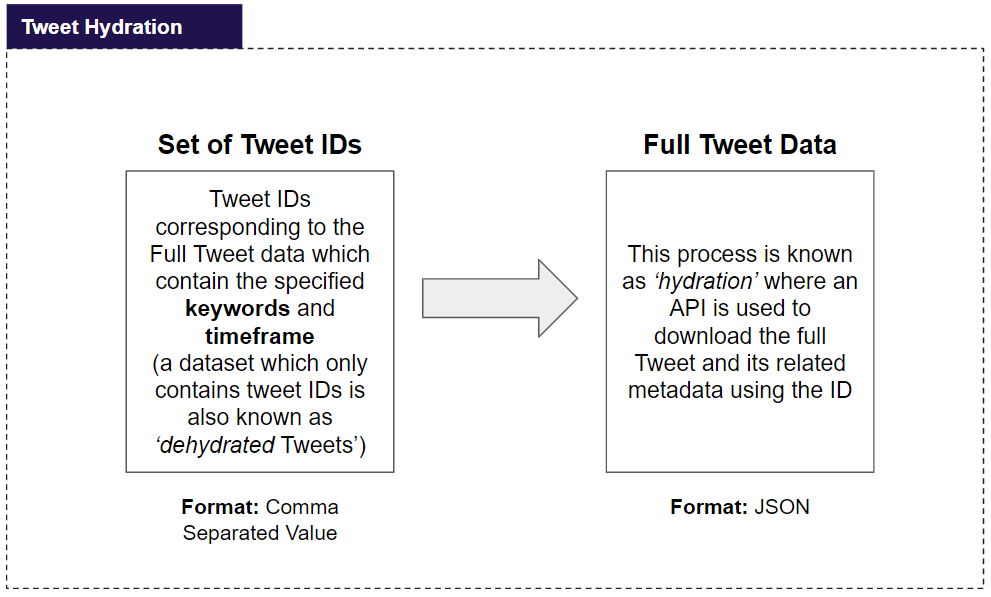
\includegraphics[width=0.75\textwidth]{figures/tweet_hydration}
\caption{Tweet hydration process} 
\label{fig:tweet_hydration}
\end{figure}

\begin{figure}[tbp]
\centering 
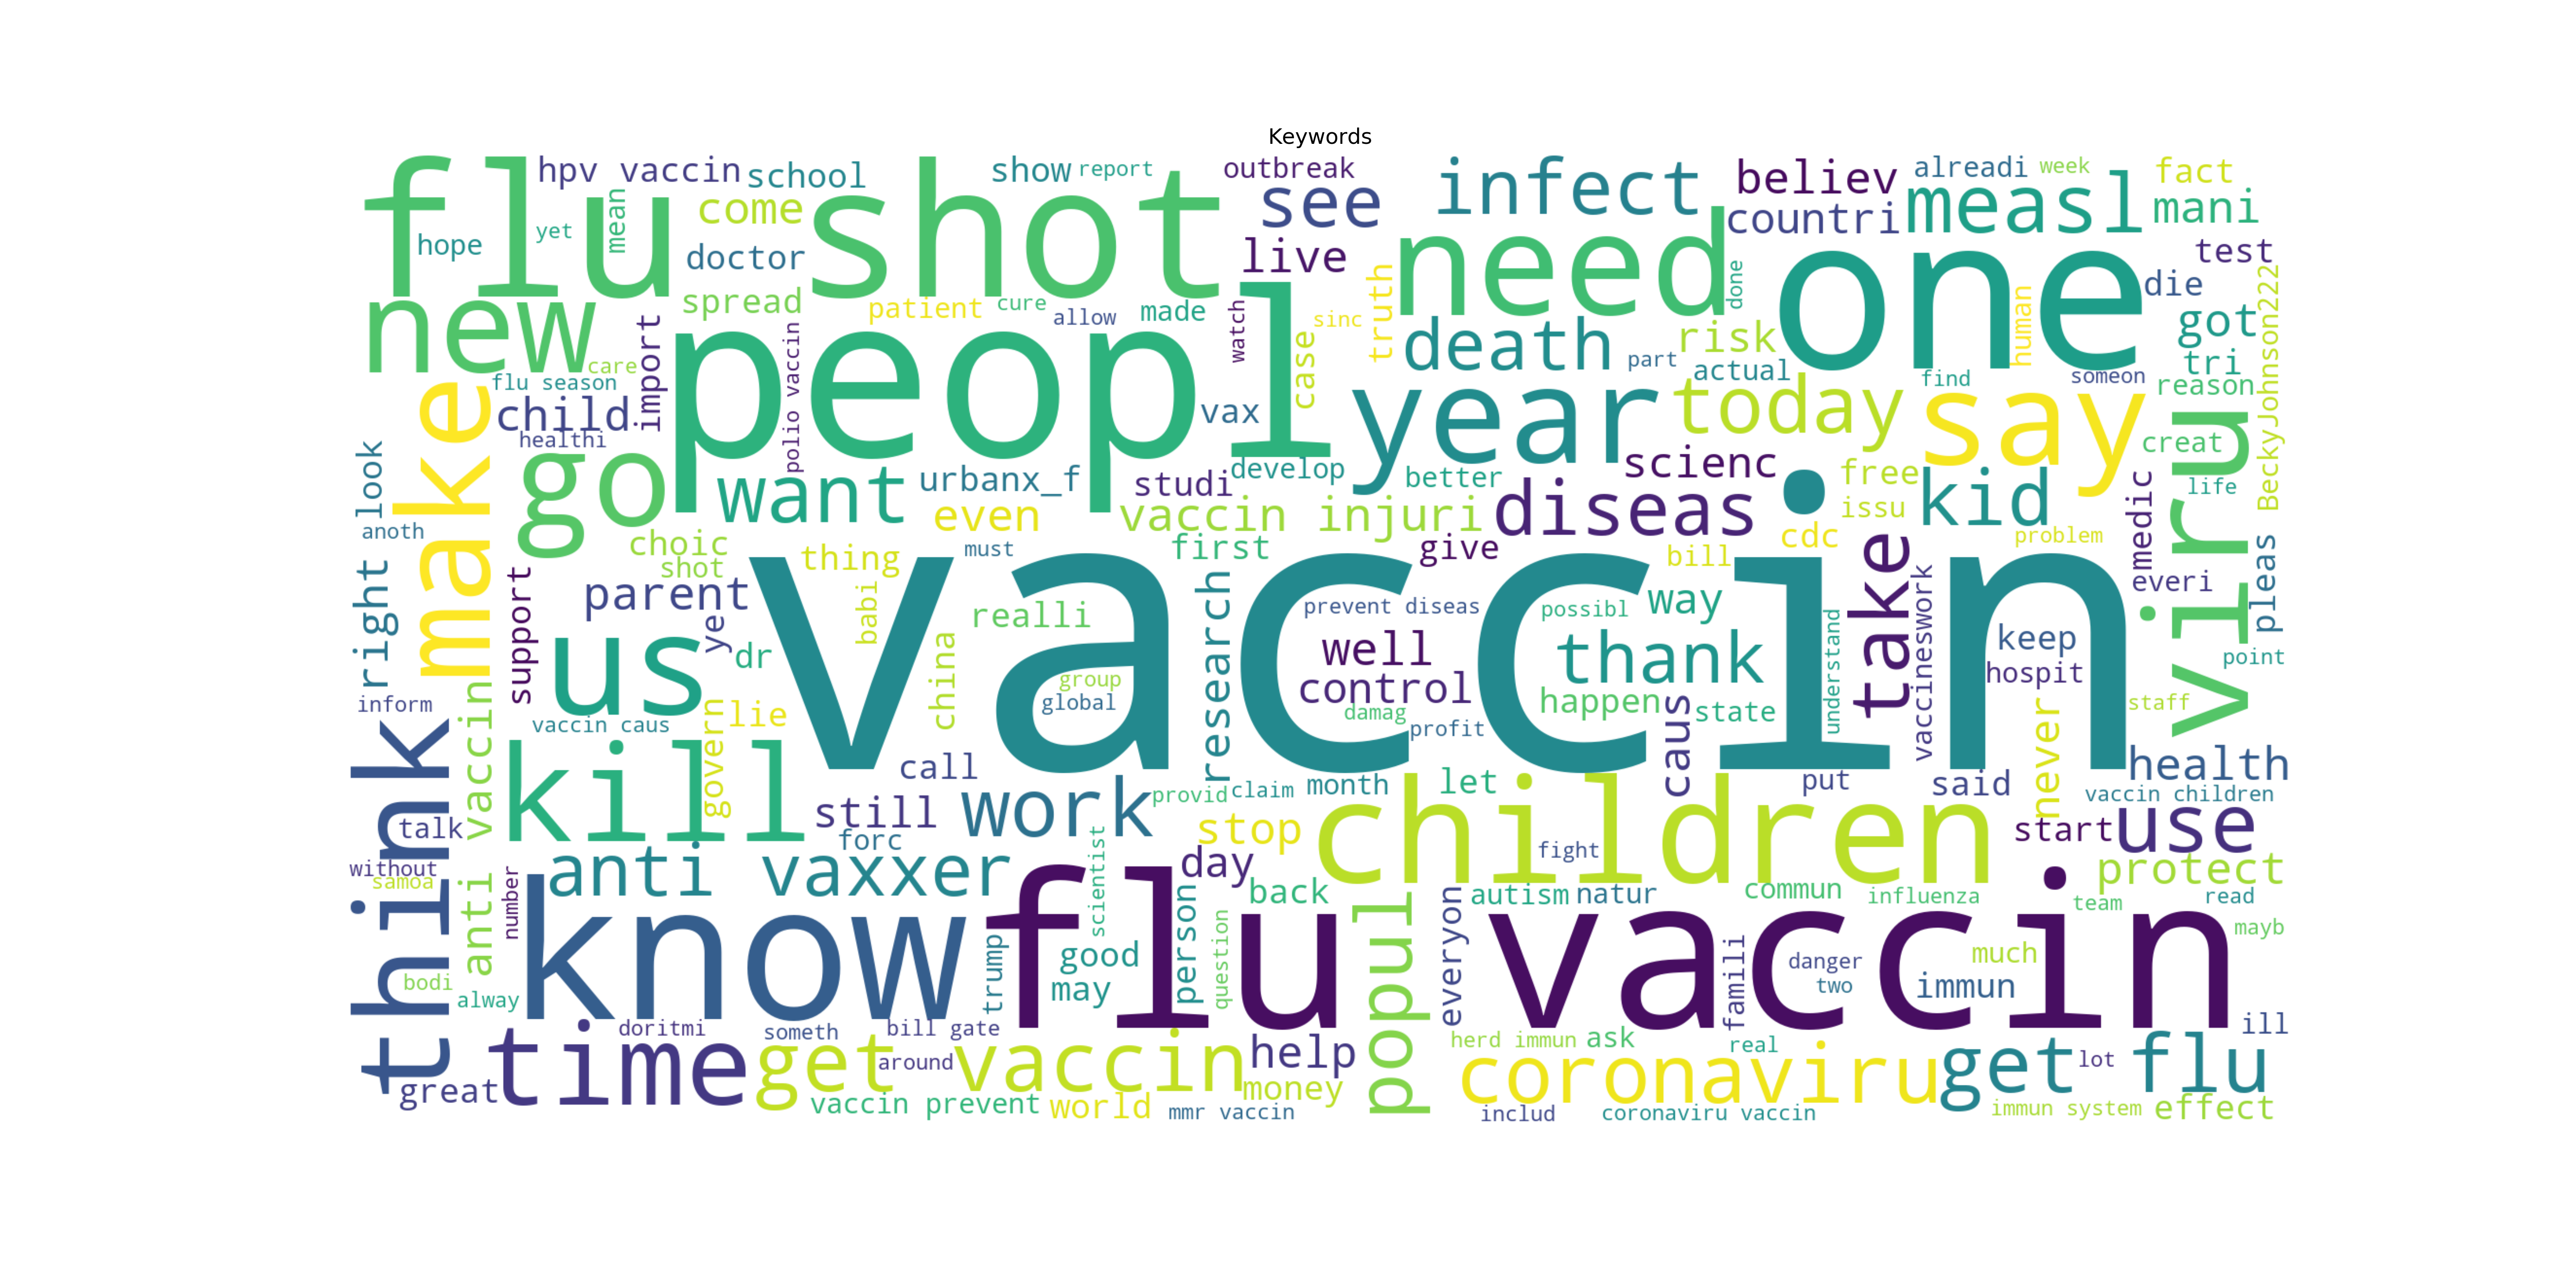
\includegraphics[width=1\textwidth]{figures/fig_word_cloud}
\caption{WordCloud of most prevalant words} 
\label{fig:fig_word_cloud}
\end{figure}


\newpage


\section{Data Pre-processing}
Figure \ref{fig:data_prepro} shows the overall end to end workflow followed for the data pre-processing. The Input for this process is the Tweets metadata in JSON format produced from the Tweet Hydration Process. The main output of this step is the exported dataset which can be used by Human annotators to label the data. 

\begin{figure}[tbp]
\centering 
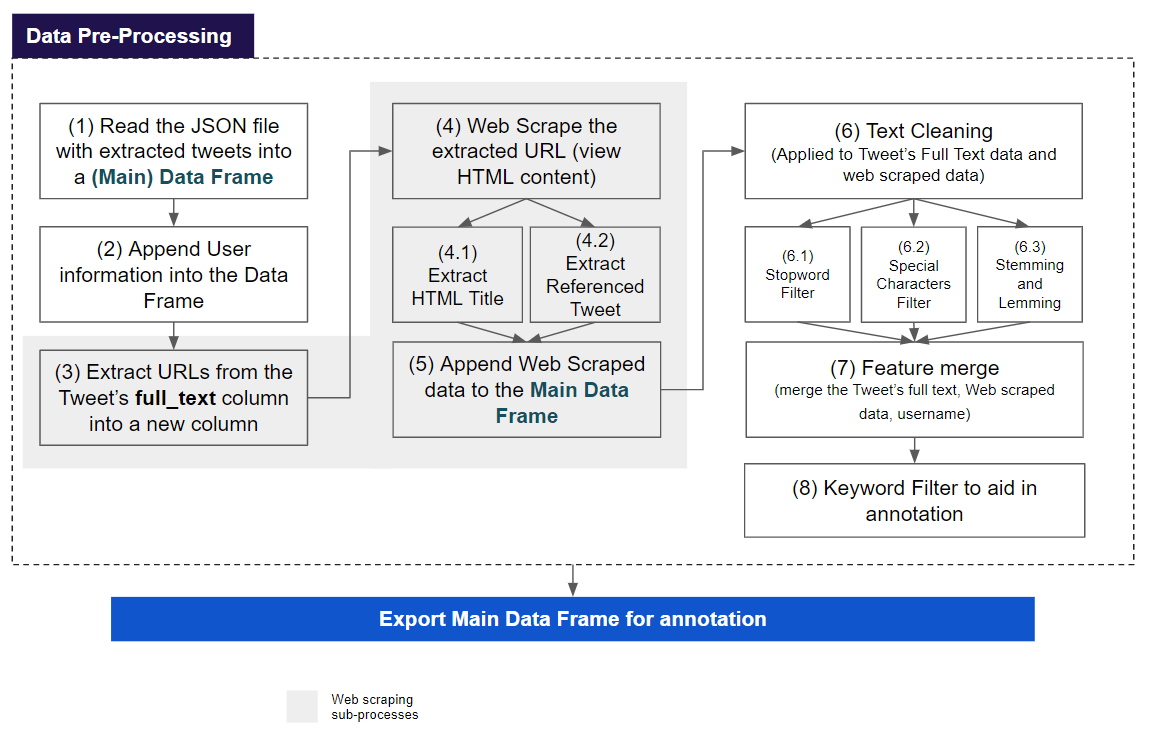
\includegraphics[width=0.75\textwidth]{figures/data_prepro}
\caption{End to end Data Pre-processing workflow} 
\label{fig:data_prepro}
\end{figure}


\subsection{JSON to Data Frame}

This section describes steps one and two in the data preprocessing workflow. 

After the Twitter ID’s were run through the API, the output resulted in a series of JSON files, all of which transcended the traditional format. A JSON (JavaScript Object Notation) filetype is a convenient way of storing and transmitting data objects.  For the purpose of this project however, each JSON must be converted into a data frame for ease of exporting to Excel later in the process. 

The program utilizes multiple user-defined functions which specifically extracts Twitter’s exported JSON files as an input.  Essentially, function main (\textit{json\_2\_df}) takes a JSON as an argument, parses out the subsets of information (child data) and appends those subsets to the main data frame (see Figure  \ref{fig:json2df}).

Once the sub-processing is completed, this newly structured dictionary is converted into a data frame that is ready to be exported to Excel. This process is repeated until all JSON files are successfully converted.  Finally, a master Excel template, which consolidates all the data exports is deposited in the same directory.


\begin{figure}[tbp]
\centering 
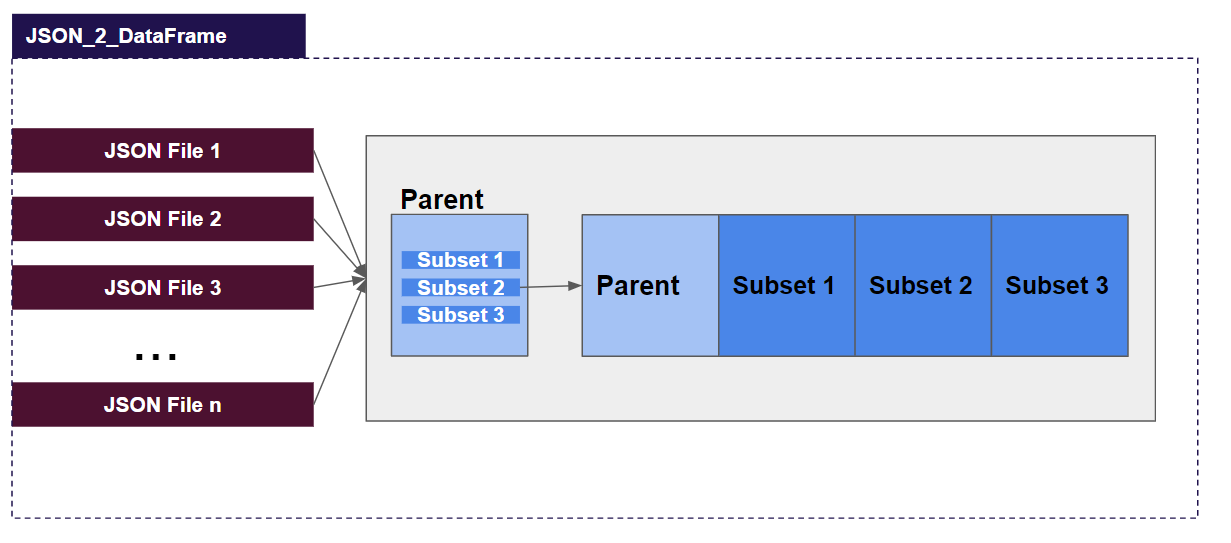
\includegraphics[width=0.75\textwidth]{figures/json2df}
\caption{Sub-process for converting JSON to Data Frame} 
\label{fig:json2df}
\end{figure}

\subsection{Web Scraping}

This section describes steps three to five in the data preprocessing workflow. 

With the entire dataset in a structured Data Frame and after some exploration of data, it can be noted that several examples of the “full\_text” feature contain one or more URLs within it. It was determined that accessing the information within these URLs would be beneficial for the overall model training and annotation; the text containing URLs accounts for approximately 22\% of the entire Data Frame, which is not insignificant. As such, the URLs were used in a web scraping process. An analysis of the URLs revealed that the majority of them could be categorized as links that lead to other tweets, or links that lead to external sites. 

The web scraping was conducted in two ways: (A) Where it directed to a Twitter link, the Tweet ID was extracted, and (B) where it lead to an external site, the HTML “Title” tag was used to extract the information. 

For (A), once the Twitter ID was extracted from the URL, the full Tweet metadata for each of the IDs was extracted using the same process described in the Data Acquisition section of this report. To simplify the representation of the architecture, a separate table was kept in memory (and externally as a file) where the unique URLs map to the specific extracted Tweet or the extracted Title.  From this point, both “Tweet” and “Title” tables were appended to the primary Data Frame by method of concatenation onto the unique URLs.  This is also illustrated in Figure \ref{fig:webscraping}

\begin{figure}[tbp]
\centering 
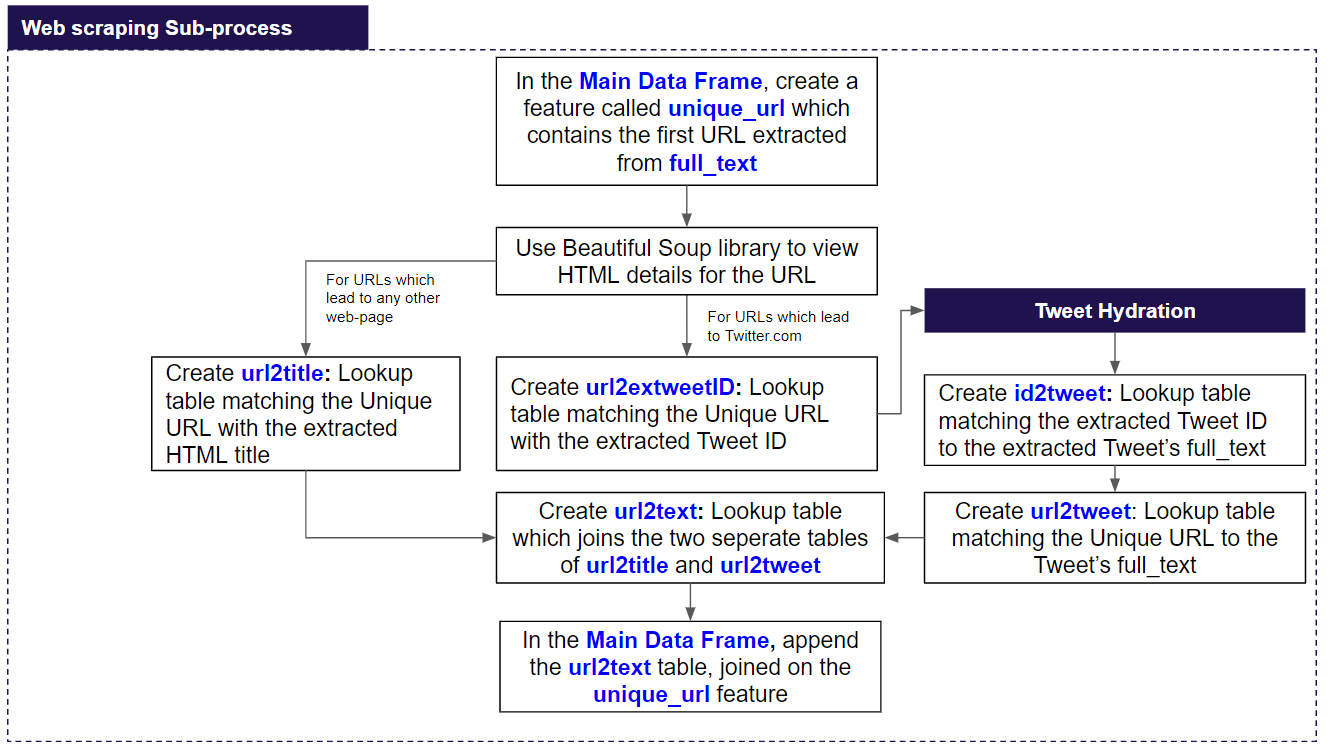
\includegraphics[width=0.75\textwidth]{figures/webscraping}
\caption{Web scraping sub-process} 
\label{fig:webscraping}
\end{figure}

\subsection{Text Cleaning}

This section describes steps six to eight in the data processing workflow.
Text cleaning involves a multitude of steps which would ultimately allow for feature X to be determined.  Feature X is a function of four features extracted from the Data Frame: “full\_text”, “scraped\_text”, “title\_text”, and “user\_screen\_name”.  Each of these feature vectors were run through a “clean\_text” function that would output vector strings that each machine learning model could use while training.   The “clean\_text” function utilizes the following NLP strategies:

\begin{itemize}
\item Replacing capital letters with their lower-case equivalent
\item Removing stop words
\item Removing all special characters 
\item Removing emojis
\item Removing URLs
\item Removing HTML tags and attributes
\item Stemming words to their root form
\item Lemming words to their root form
\end{itemize}

After each of the feature vectors were run through the clean\_text function, their outputs would recategorize them as “cleaned”.  As a result, feature X can be defined as a concatenated function of the following:

\begin{verbatim} 
X = df[full_text_cleaned] + df[scraped_text_cleaned] +
df[title_text_cleaned] + df[user_screen_name_cleaned]
\end{verbatim}

Feature X must include both \textit{scraped\_text\_cleaned} and \textit{title\_text\_cleaned}  so that the machine learning models can understand the subject or context of the URLs posted; having just the full text with no context is in most cases, not enough to go by. The username of the tweet is also appended  as it may serve as an important feature to aid in the model’s training (i.e. if the user has a history of Tweeting vaccine misinformation, the model can learn the pattern of the (anonymized) user and infer that future tweets from this individual may also be misinformation).


Finally, before the data can be exported into a user friendly file format for the purpose of human annotation; a function is applied which determines if there are any positive or negative keywords within the full\_text, or if the Tweet was produced by a user which had previously produced some polarizing views. During the first round of annotation, we discovered that it is more likely that the Tweets with positive keywords will have a more positive or neutral sentiment, whereas it is more likely that the Tweets with negative keywords will have some negative sentiment, or even misinformation. Thus, the intent for applying this function is to support the annotators during the annotation process. The list of positive and negative keywords is provided in the appendix; the username list is not provided to protect user privacy. This process of labeling the keywords allows for a more focused annotation process as opposed to annotating chronologically. 

\begin{figure}[tbp]
\centering 
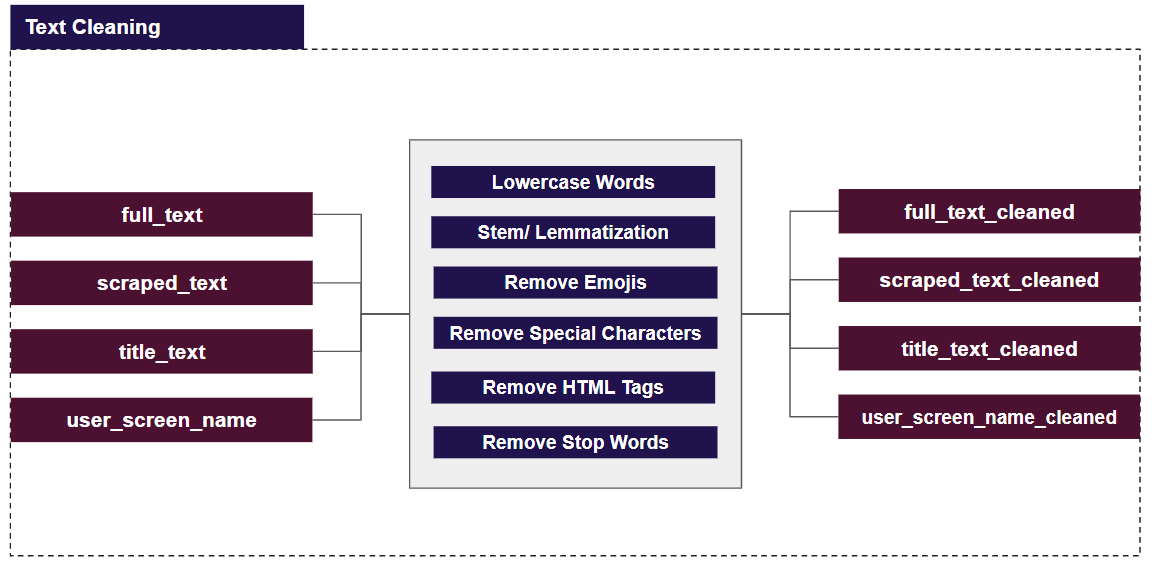
\includegraphics[width=0.75\textwidth]{figures/text_cleaning}
\caption{Text Cleaning Sub-process} 
\label{fig:text_cleaning}
\end{figure}

\section{Data Annotation}

For this project, the annotation was conducted by two main annotators, and a third person(s) acting as a tie-breaker should there be a mismatch between the original two annotators’ labels – a critical task to maintain high inter-rater agreement for vaccine sentiment. The data was labelled into five classes which captured the different levels of misinformation as it relates to vaccines. These are described in Tables \ref{tbl:class_labels} and Table \ref{tbl:class_examples}


out of the 45,551 downloaded Tweets, the following is the final count of the annotated tweets (n=7987). As seen in Table \ref{tbl:class_labels}, there is an overwhelming imbalance of Tweets with a positive sentiment tweets as compared to those with misinformation, which justifies the need for under-sampling. This will be further explored in the next section with a comparison of under-sampled results with no under-sampling. 



\begin{table}[tbp]
\centering
\begin{tabularx}{\linewidth}{l X r}
\toprule
Class Label & Definition & Counts\\
\midrule

0 & The assessment of the risk related to acquiring vaccine-related injuries, and the severity of vaccine-related injuries  & 4409 \\
1 & Immunization related content that does not express opposition or support towards vaccines, usually in the form of a news report  & 729 \\
2 & The assessment of the risk related to acquiring vaccine-related injuries, and the severity of vaccine-related injuries  & 1056\\
3 & Opinions that demonstrate conspiratorial thinking and ideologies (e.g. political, religious, and social norms) that are not misinformation related to science & 1165 \\ 
4 & Tweets that do not belong to any of the above, or irrelevant, not human vaccines & 628\\
N/A & Tweets that are no longer available, in non-English, or account suspended & (Removed) \\

\bottomrule
\end{tabularx}
\caption{Class Labels}
\label{tbl:class_labels}
\end{table}


\begin{table}[tbp]
\centering
\begin{tabularx}{\linewidth}{ l X X X X}
\toprule
    Class Label & Common Concerns &Categorization & Sample Tweets\\
\midrule

0 &	Pro-vaccine tweets – no misinformation &	Content that supports vaccination, expect a lot of hostile and sarcastic content & \textit{Great, I can now experience measles because of crazy anti-vaxxers.} \\
\midrule

1 & Neutral sentiment tweets – no misinformation & Content that neither endorse nor oppose vaccination &  \textit{Vaccine supply shortage in India}  \\
\midrule

2 & The dosage, timespan of injection, and ingredients in vaccines overwhelm the immune system, causing harm to the body & Perceived risk and severity of getting vaccinated & \textit{My baby experience seizures after she received 6 shots in 2 days.} \\
\midrule
2&Vaccines increase the risk of autism, cancer, infertility &Perceived risk and severity of getting vaccinated & \textit{HPV shots made women in Denmark involuntarily self-abort, a Cochrane study shows}\\
\midrule
2&Natural immunity is better than artificial immunity&Perceived benefit of not receiving vaccination &\textit{I never get sick and I wasn't vaccinated}\\
\midrule
2&More vaccinated than unvaccinated people get sick, vaccines do not work&Perceived benefit of not receiving vaccination & \textit{the only times I got sick was when I was vaccinated}\\
\midrule

3&Big Pharma is making money off of sick people &Ideology and conspiracy theory related & \textit{Pharmaceuticals are ramping up vaccine creation, covid-19 is man-made, coincidence much?}\\
\midrule
3&Vaccination is genocide&Ideology and conspiracy theory related &\textit{Bill Gates is killing millions of innocent African children with the polio vaccine}\\
\midrule
4&Other& Tweets that do not belong to any of the above, or irrelevant, not human vaccines& \textit{}\\

\bottomrule
\end{tabularx}
\caption{Class examples}
\label{tbl:class_examples}
\end{table}

\section{NLP \& Machine Learning Methods}
\subsection{Sources of Measure}

For this \textit{study, accuracy, precision, recall} and \textit{f1-score} were all taken into consideration. Each of these evaluation metrics can be defined using a simple confusion matrix layout.  A confusion matrix is composed of four classification cells (defined below) based on 2-dimensional axes: \textit{predicted value (PV)} and \textit{actual value (AV)}. 

The four classification cells in a binary confusion matrix is described in Table \ref{tbl:cm_desc} and a sample confusion matrix is shown in Figure \ref{fig:cm_sample}.

Each cell in the confusion matrix is represented by an integer number which counts the number of TP’s, FP’s, FN’s or TN’s.  Therefore, it is ideal if there are more TP’s and TN’s than FP’s and FN’s.  The confusion matrix should have higher counts along its downward diagonal (ie. blue squared cells from the image above).

The confusion matrix can be used for multi-classification problems in addition to just binary.  So long as each class is sequentially placed along the x and y axes such that their corresponding actual and predicted values meet in the diagonal, this will not be an issue.  An example of a five-class confusion matrix can be seen in Figure \ref{fig:cm_5class}. From the confusion matrix, each evaluation metrics can be used in the machine learning process and defined. Table \ref{tbl:eval_metrics} shows the description for each evaluation metric. By evaluating each of these evaluation metrics, the output of the model will display a much more holistic view of the machine learning model and its performance. 



\begin{table}[tbp]
\centering
\begin{tabularx}{\linewidth}{ l X}
\toprule
   Classification Cells & Description \\
\midrule

True-Positive (TP) & If the PV predicts True and the AV is True.\\
True-Negative (TN) & If the PV predicts False and the AV is False.\\
False-Positive (FP) & If the PV predicts True and the AV is False.\\
False-Negative (FN) & If the PV predicts False and the AV is True.\\

\bottomrule
\end{tabularx}
\caption{Confusion Matrix Description}
\label{tbl:cm_desc}
\end{table}


\begin{figure}[tbp]
\begin{center}
\subfigure[Confusion Matrix Sample]{
    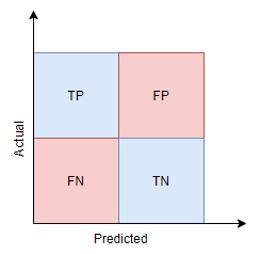
\includegraphics[scale=1]{figures/cm_sample}
    \label{fig:cm_sample}
}
\subfigure[Five Class Confusion Matrix]{
    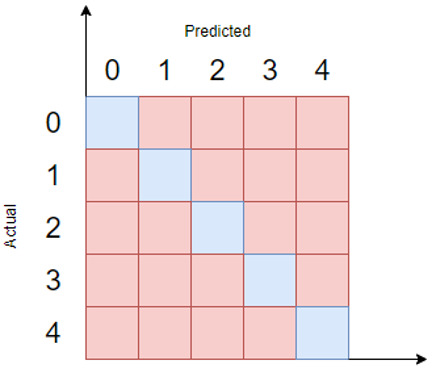
\includegraphics[scale=0.68]{figures/cm_5class}
    \label{fig:cm_5class}
}

\end{center}
\caption{Confusion Matrix Examples}
\label{fig:cm}
\end{figure}



\begin{table}[tbp]
\centering
\begin{tabularx}{\linewidth}{ l X X}
\toprule
   Evaluation Metrics & Definition & Calculation\\
\midrule

Accuracy & Number of correctly identified predicted values over total number of predictions. & TP + TN /(TP + TN + FP + FN) \\
Precision & Number of correctly identified positive cases over total number of predicted positive cases. & TP/(TP + FP)\\
Recall & Number of correctly identified positive cases over the total number of cases that should have been positively identified.  & TP/(TP + FN)\\
F1-Score &Represents the harmonic mean of both the precision and recall. & 2TP/(2TP + FP + FN)\\

\bottomrule
\end{tabularx}
\caption{Evaluation metrics Description}
\label{tbl:eval_metrics}
\end{table}

\newpage

\subsection{Model Details}
All machine learning models have been developed in Python 3.X while using the Jupyter Notebook and Spyder IDE’s.  

The machine learning training for this project was split up into five distinct models. Each model grouped the data in either five, four or three classes – even as the data was annotated against five classes. The details of how the classes are grouped is provided in Table \ref{tbl:model_details}, and the overall processing is visualized in Figure \ref{fig:ml_train}

This split into five models was partially done so to address the class imbalance present within the annotated data, and partially to understand the impact of increased training examples within a class. It is generally expected that with a higher number of classes, the model accuracy (and the evaluation of other evaluation metrics) is expected to go down.  Reduced model accuracy was observed in Mønsted and Lehmann’s study where they used tweets to study vaccine discourse.
For models 3 and 5, the hypothesis being tested is that tweets which have little to do with vaccines (class 4) could be considered tweets which have a neutral sentiment towards vaccines. Whereas for Models 2 and 4, the hypothesis is that it is better to remove class 4 entirely from the dataset. The model results are intended to provide support for either of the hypotheses. 



\begin{table}[tbp]
\centering
\begin{tabularx}{\linewidth}{ l X}
\toprule
   Model & Description \\
\midrule

Model 1 & All classes used (five classes in total), randomly under-sampled class 0 to count of class 3\\
Model 2 & Removing class 4 form the dataset (four classes in total), randomly under-sampled class 0 to count of class 3\\
Model 3 & Converting class 4 into class 1 (four classes in total), randomly under-sampled class 0 to count of (new) class 1\\
Model 4 & Removing class 4 from the dataset, converting class 3 into class 2 (three classes in total), randomly under-sampled class 0 to count of (new) class 2\\
Model 5 & Converting class 4 into class, converting class 3 into class 2 (three classes in total), randomly under-sampled class 0 to count of (new) class 2\\

\bottomrule
\end{tabularx}
\caption{Model Details}
\label{tbl:model_details}
\end{table}

\newpage

\begin{figure}[tbp]
\centering 
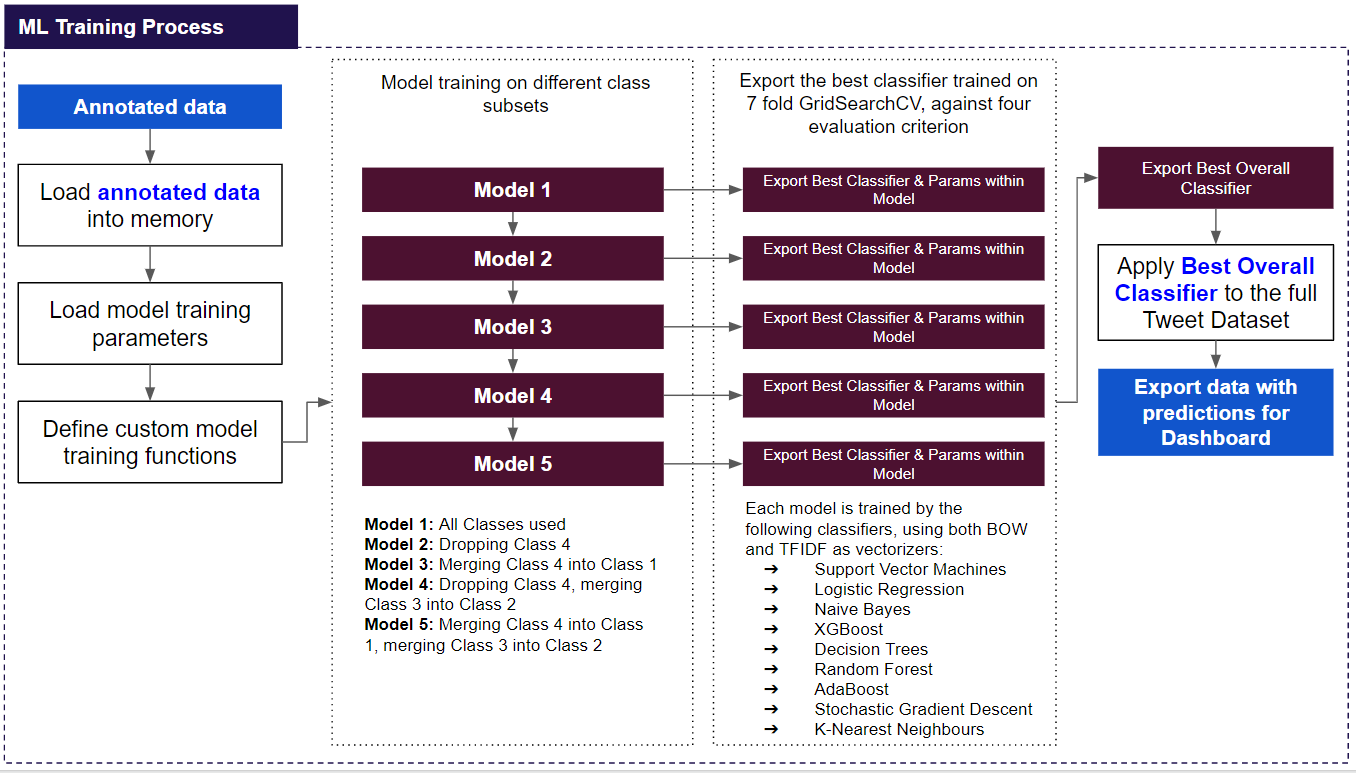
\includegraphics[width=1\textwidth]{figures/ml_train}
\caption{Machine learning training process} 
\label{fig:ml_train}
\end{figure}


\begin{table}[tbp]
\centering
\begin{tabularx}{\linewidth}{ l X}
\toprule
   Class Label & Count \\
\midrule
0 & NS: 4409 \newline US: 1165 \footnote{NS = No Sampling. US = Under-sampled. Under-sampled class count has been randomly under sampled to be equal to the count of the second highest class count.}\\
1 & 729\\
2 & 1056\\
3 & 1165\\
4 & 628\\
\bottomrule
\end{tabularx}
\caption{Model 1 Details}
\label{tbl:model1_details}
\end{table}

\begin{table}[tbp]
\centering
\begin{tabularx}{\linewidth}{ l X}
\toprule
   Class Label & Count \\
\midrule
0 & NS: 4409 \newline US: 1109 \\
1 & 729\\
2 & 1056\\
3 & 1165\\

\bottomrule
\end{tabularx}
\caption{Model 2 Details}
\label{tbl:model2_details}
\end{table}

\begin{table}[tbp]
\centering
\begin{tabularx}{\linewidth}{ l X}
\toprule
   Class Label & Count \\
\midrule
0 & NS: 4409 \newline US: 1357\\
1 & 1357\\
2 & 1056\\
3 & 1165\\
\bottomrule
\end{tabularx}
\caption{Model 3 Details}
\label{tbl:model3_details}
\end{table}

\begin{table}[tbp]
\centering
\begin{tabularx}{\linewidth}{ l X}
\toprule
   Class Label & Count \\
\midrule
0 & NS: 4409 \newline US: 2221\\
1 & 729\\
2 & 2221\\

\bottomrule
\end{tabularx}
\caption{Model 4 Details}
\label{tbl:model4_details}
\end{table}

\begin{table}[tbp]
\centering
\begin{tabularx}{\linewidth}{ l X}
\toprule
   Class Label & Count \\
\midrule
0 & NS: 4409 \newline US: 2221\\
1 & 1357\\
2 & 2221\\

\bottomrule
\end{tabularx}
\caption{Model 5 Details}
\label{tbl:model5_details}
\end{table}

\newpage

\subsection{Model Training}
A total of nine different classifiers were trained and compared for each model, as described in Table \ref{tbl:classifiers}. The SKLearn library was utilized to implement and train the classifiers with 7-fold Cross Validation using GridSearchCV against four different evaluation metrics, and various parameters as noted above. Furthermore, each classifier was trained using two vectorization methods: Bag-of-Words (BOW) and Term Frequency-Inverse Document Frequency (TF-IDF). The best model for each classifier by evaluation metrics and vectorizer is exported into a specified folder path for later use if needed, along with a summary of the evaluation metrics. This results in 72 classifiers being exported into .sav files for each model using the ‘pickle’ Python library.  



\begin{table}[tbp]
\centering
\begin{tabularx}{\linewidth}{ l X}
\toprule
   Classifier & Parameters Explored \\
\midrule
Support Vector Machines (SVM) & C: \textit{1,10,20,30} \newline kernel: \textit{rbf, linear} \newline \\
Logistic Regression & Solver: \textit{lbfgs} \newline multi\_class: \textit{multinomial} \newline C: \textit{1,5,10} \newline \\
Naive Bayes & Alpha: \textit{0, 1}\newline  \\
XGBoost & max\_depth: \textit{10,20,50,100}, \newline min\_child\_weight: \textit{5, 10, 15}\newline  \\
Decision Trees & max\_depth: \textit{10,20,30,100}, \newline criterion: \textit{gini, entropy} \newline \\
Random Forest & n\_estimators: \textit{50,100,200}, \newline max\_depth: \textit{5,10,20,100} \newline \\
AdaBoost & n\_estimators: \textit{200} \newline \\
Stochastic Gradient Descent & loss: \textit{hinge}, \newline penalty: \textit{l2}, \newline max\_iter: \textit{5,10,15} \newline \\
K-Nearest Neighbours & n\_neighbors: \textit{1,5,10} \newline \\

\bottomrule
\end{tabularx}
\caption{List of classifiers and their hyper-parameters}
\label{tbl:classifiers}
\end{table}

\subsection{Bag-of-words (BOW)}
BOW is a vectorization technique that consolidates all of the known tokenized words from each sample and compiles them into a large matrix (i.e. total number of samples x total number of feature tokens). By organizing words from the corpus in this manner, the machine learning model is able to recognize trends and associate certain words with different class labels.
One common issue with BOW however is that the matrix will often become very large and sparse; that is to say, the majority of cells within the matrix will contain a 0 (i.e. the number of time a specific word may appear in the sentence is zero).This is because once the text has been cleaned, certain Tweets will contain specific words that other users might not have used in their respective posts.  As a result, it may be difficult for the machine learning model to learn to associate important words with a particular class label outcome.  An example of a BOW matrix can be found in Figure \ref{fig:bow}.

\begin{figure}[tbp]
\centering 
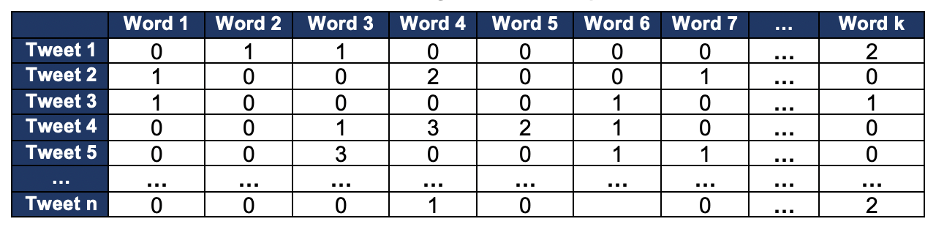
\includegraphics[width=1\textwidth]{figures/bow}
\caption{Bag of words example} 
\label{fig:bow}
\end{figure}

\subsection{Term Frequency-Inverse Document Frequency (TF-IDF)}
TF-IDF is a vectorization technique that weights the importance of words based on the number of times they appear within each Tweet or “document”.  If a particular word is common among all documents, its relative importance compared to other words will decrease. 

Similarly to BOW, TF-IDF will start by counting the number of times a particular word appears in a document.  This denotes the “term frequency” or TF.  Each document will have its own TF value for every word in the entire corpus.  

Next, it looks at the IDF (inverse document frequency) which is the value used to weight the significance of the word.  The IDF can be calculated as follows:
\[ IDF = \log(N/DF) \]
Where \textit{N} = Total number of documents, \textit{DF} = Total number of documents containing the specific word. DF can never exceed N, and so if DF = N, then the relative importance of that word will be weighted as 0.

\newpage
\subsection{Model Results}
The model results are presented in the subsequent pages. Each model’s evaluation is presented with both under-sampled and non-sampled data. The confusion matrix displayed at the end of each cell is represented by the best classifier, according the to the grid search.  As previously discussed, the evaluation metrics include accuracy (blue), precision (green), recall (red) and f1-score (orange), each of which was captured as a percentage and displayed in a horizontal bar graph.   


\begin{figure}[tbp]
\begin{center}

\subfigure[Model 1 with under-sampling - BOW]{
    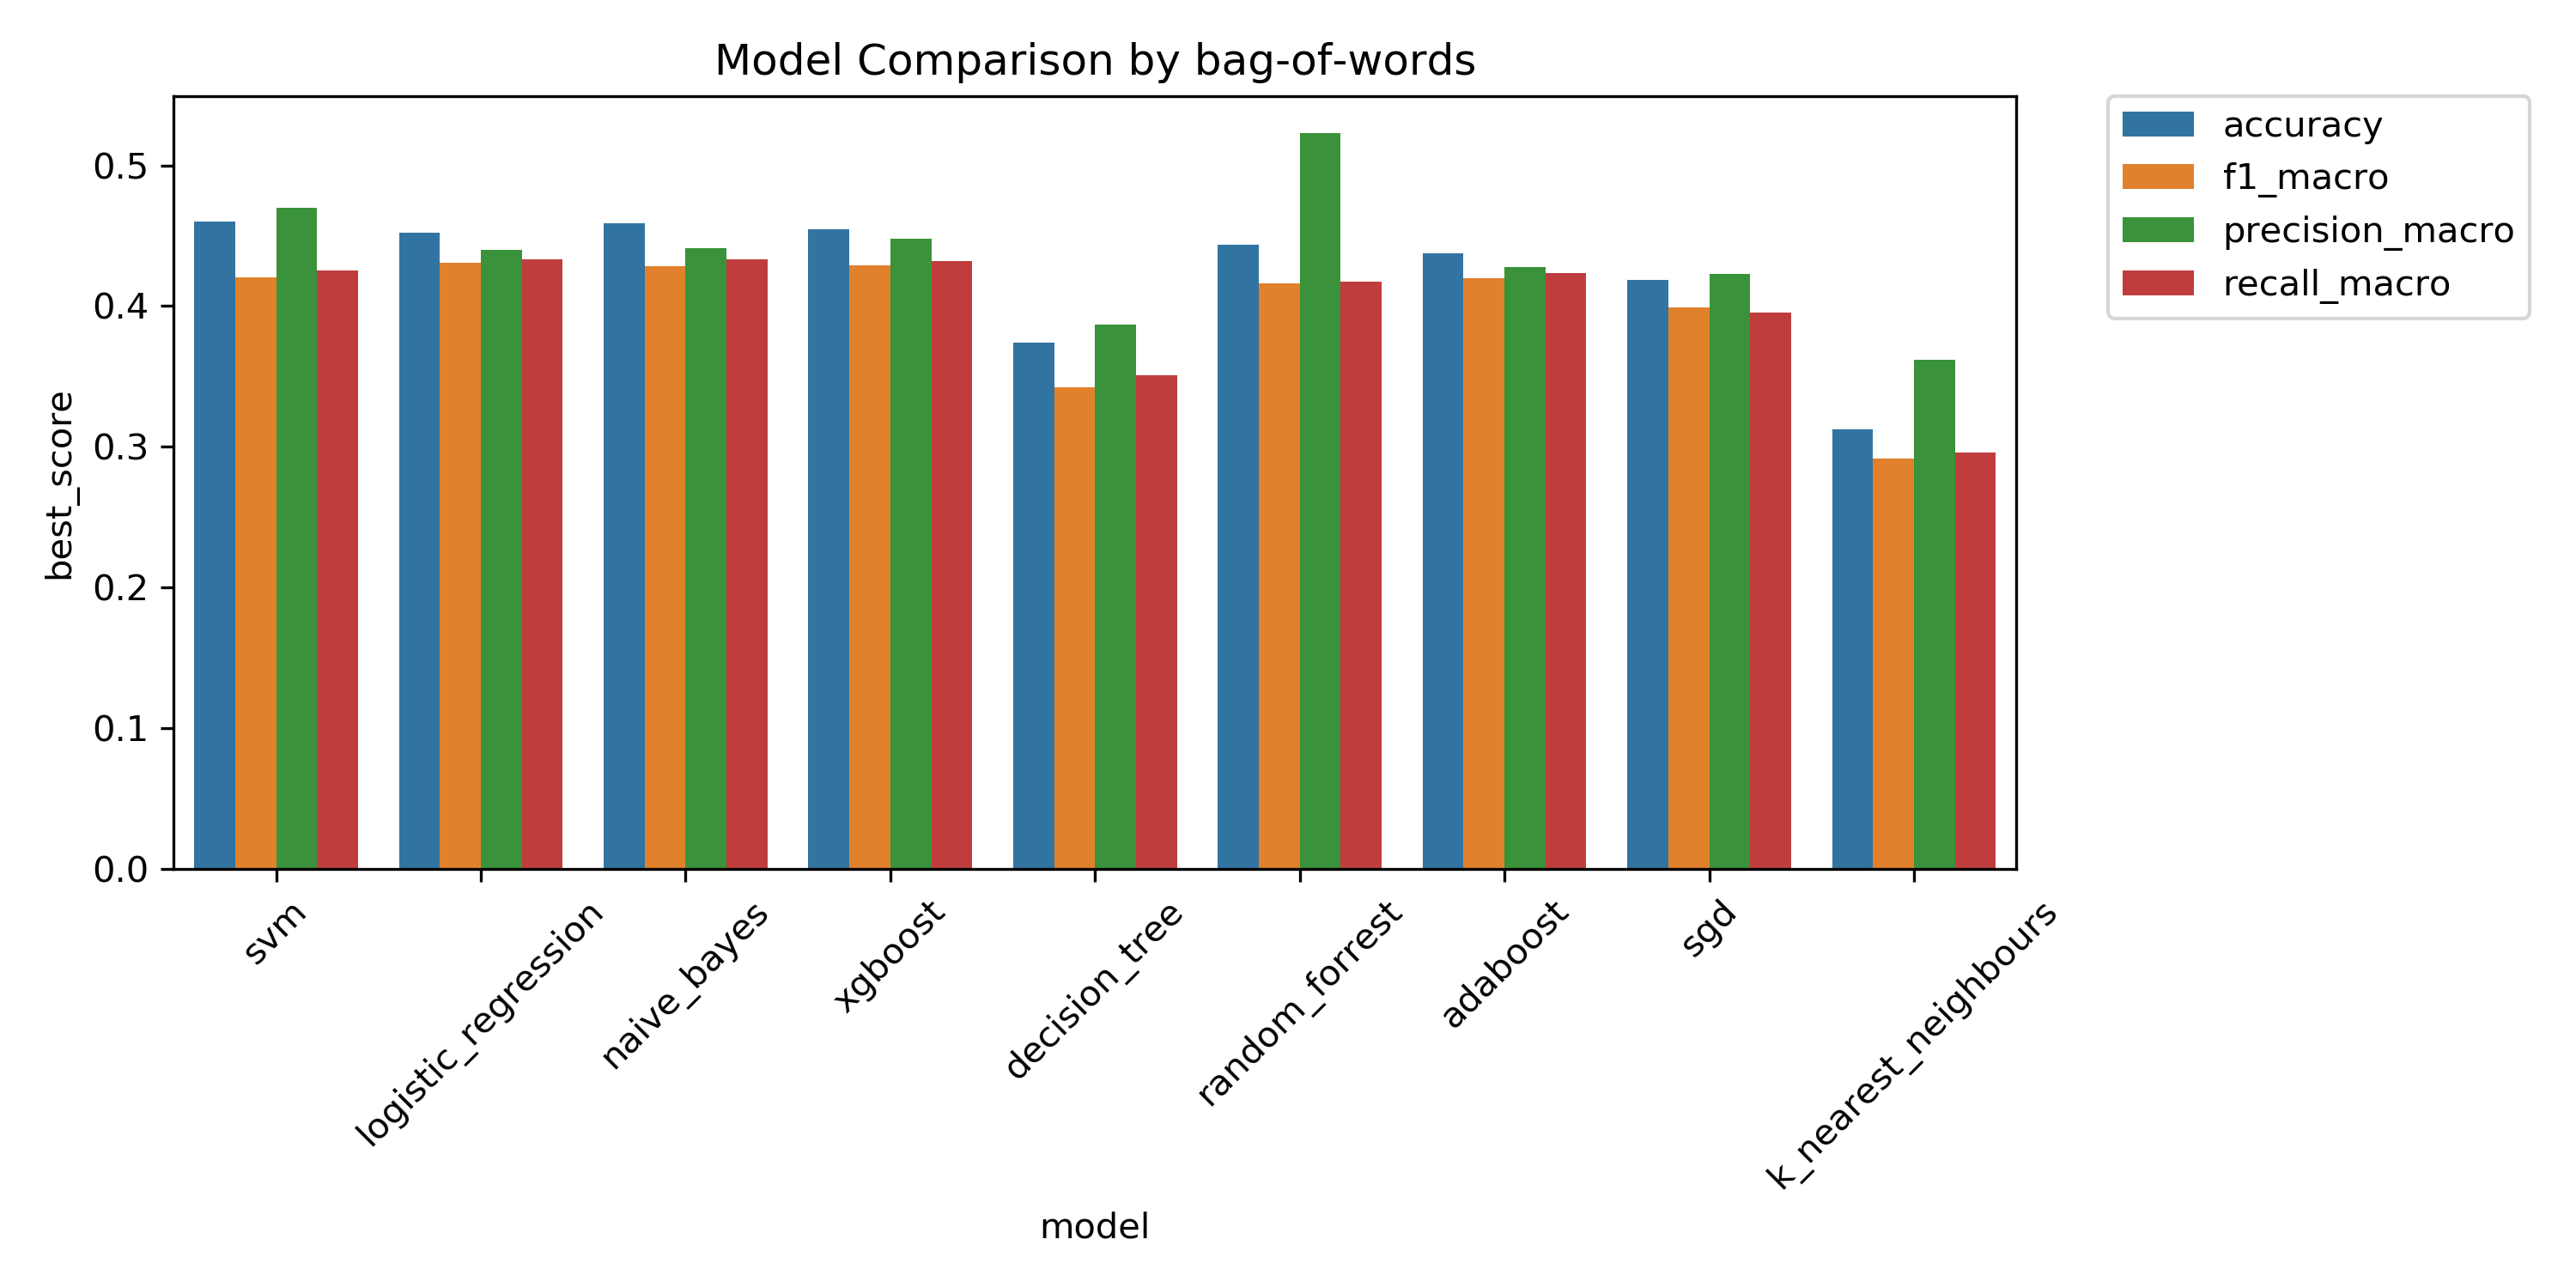
\includegraphics[scale=0.3]{figures/us_m1bow}
    \label{fig:us_m1bow}
}
\subfigure[Model 1 without under-sampling - BOW]{
    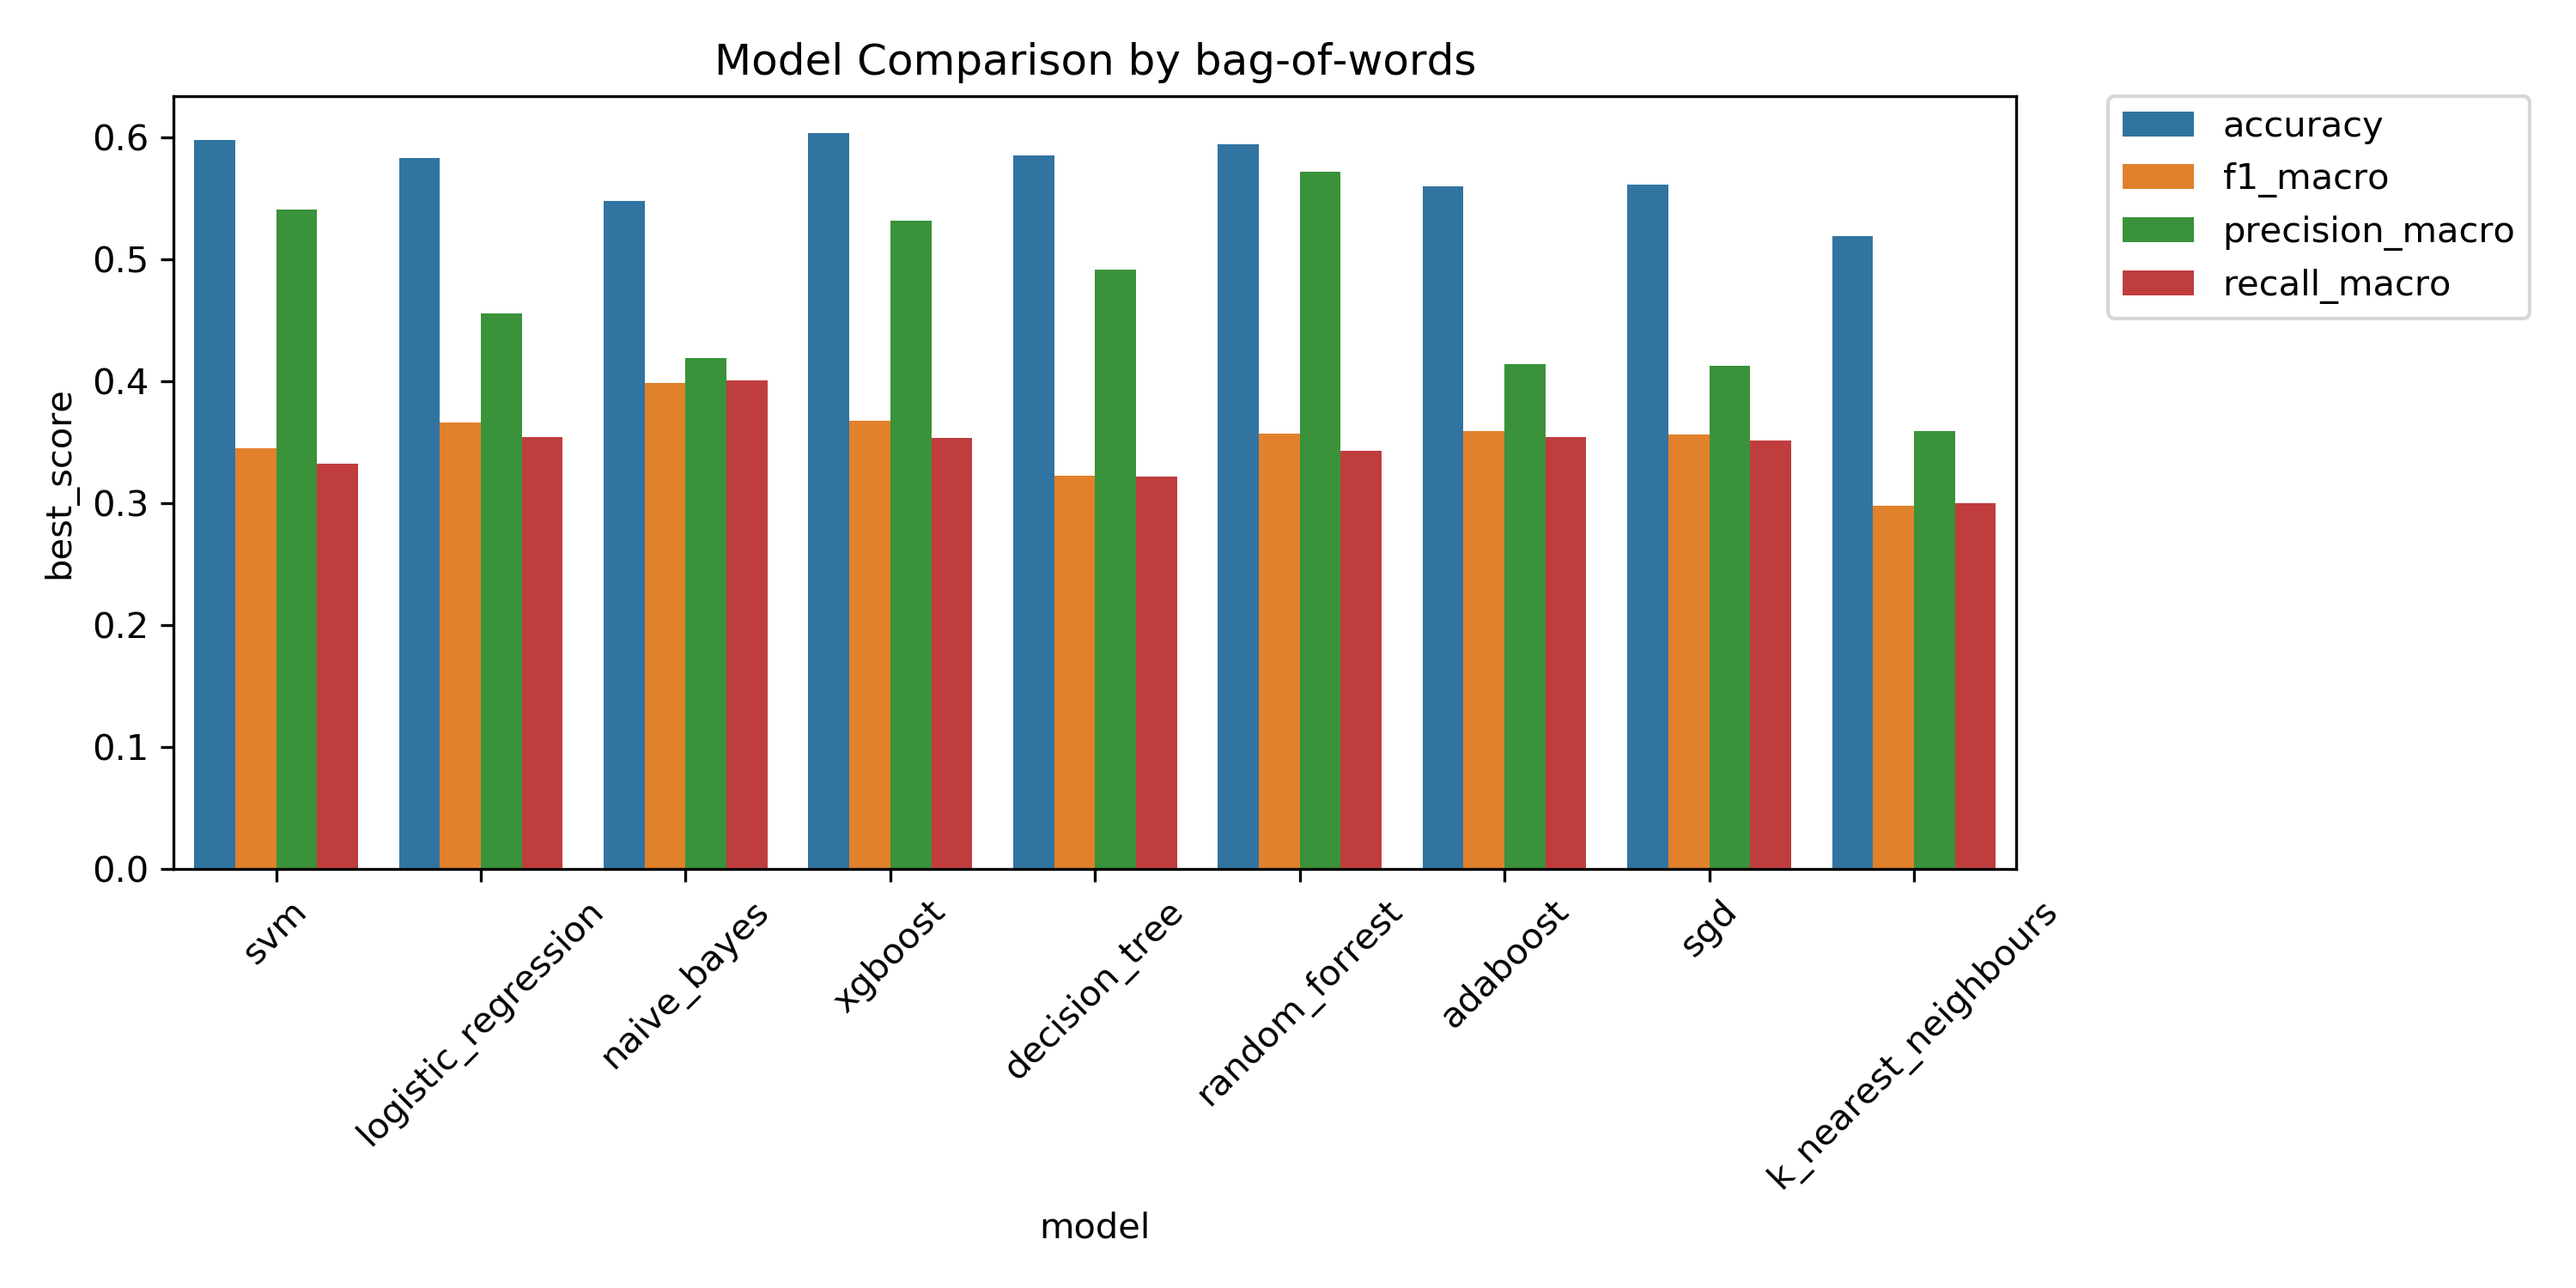
\includegraphics[scale=0.3]{figures/ns_m1bow}
    \label{fig:ns_m1bow}
}
\subfigure[Model 1 with under-sampling - TFIDF]{
    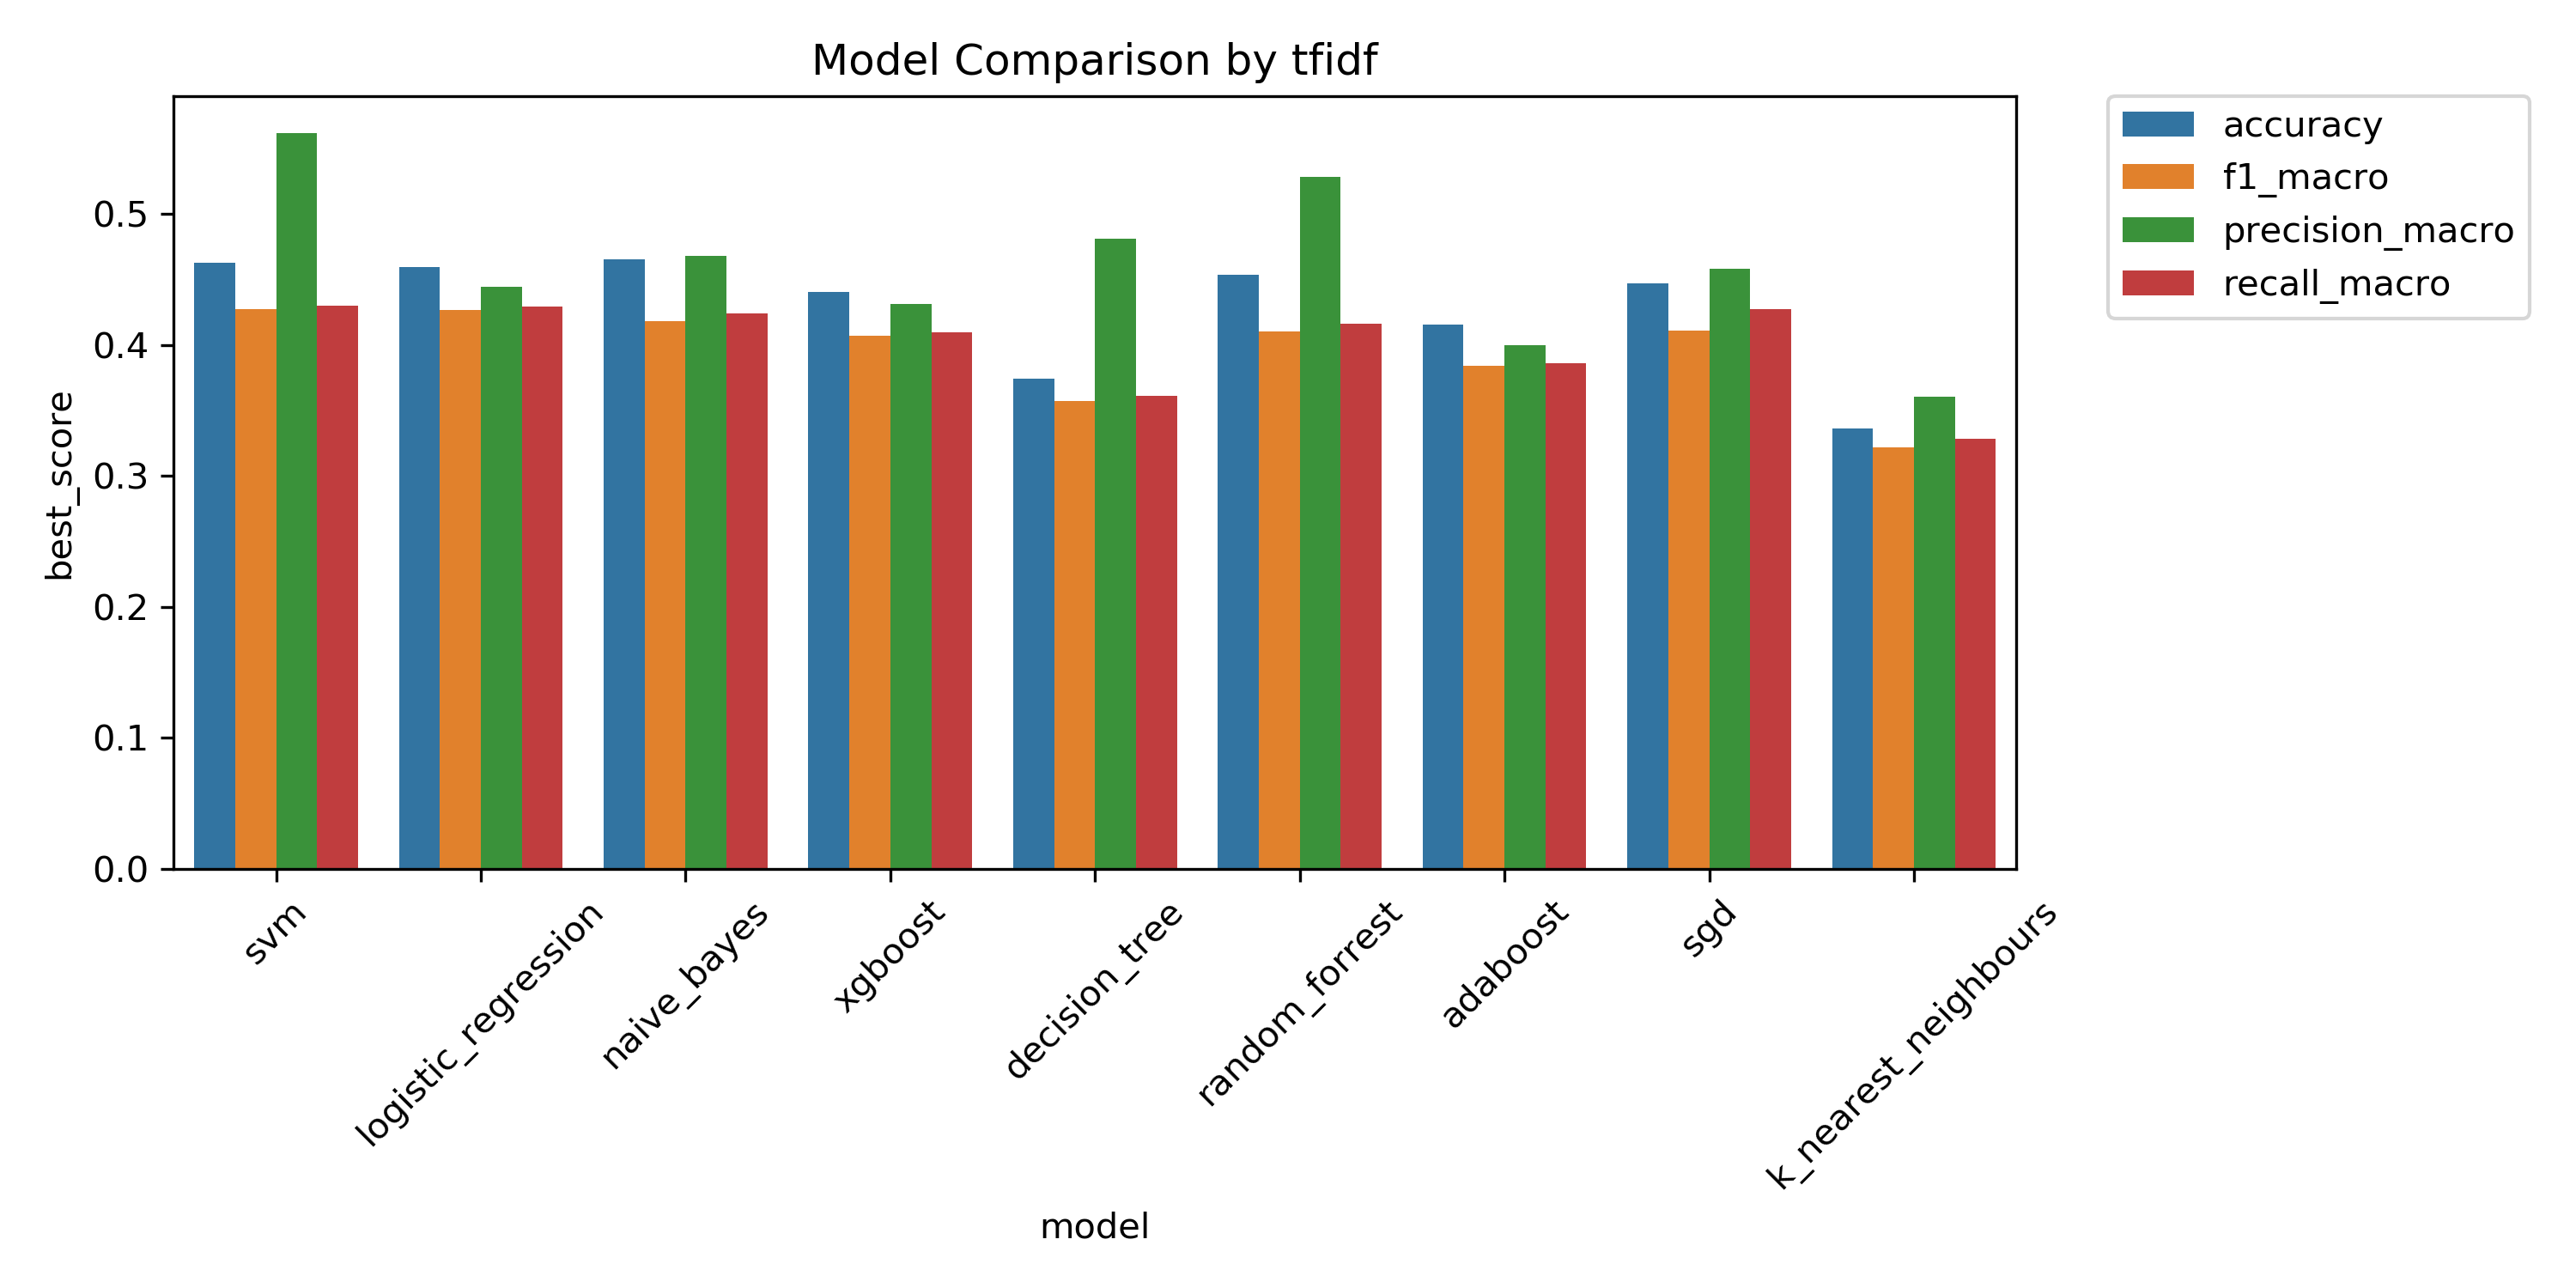
\includegraphics[scale=0.3]{figures/us_m1tfidf}
    \label{fig:us_m1tfidf}
}
\subfigure[Model 1 without under-sampling - TFIDF]{
    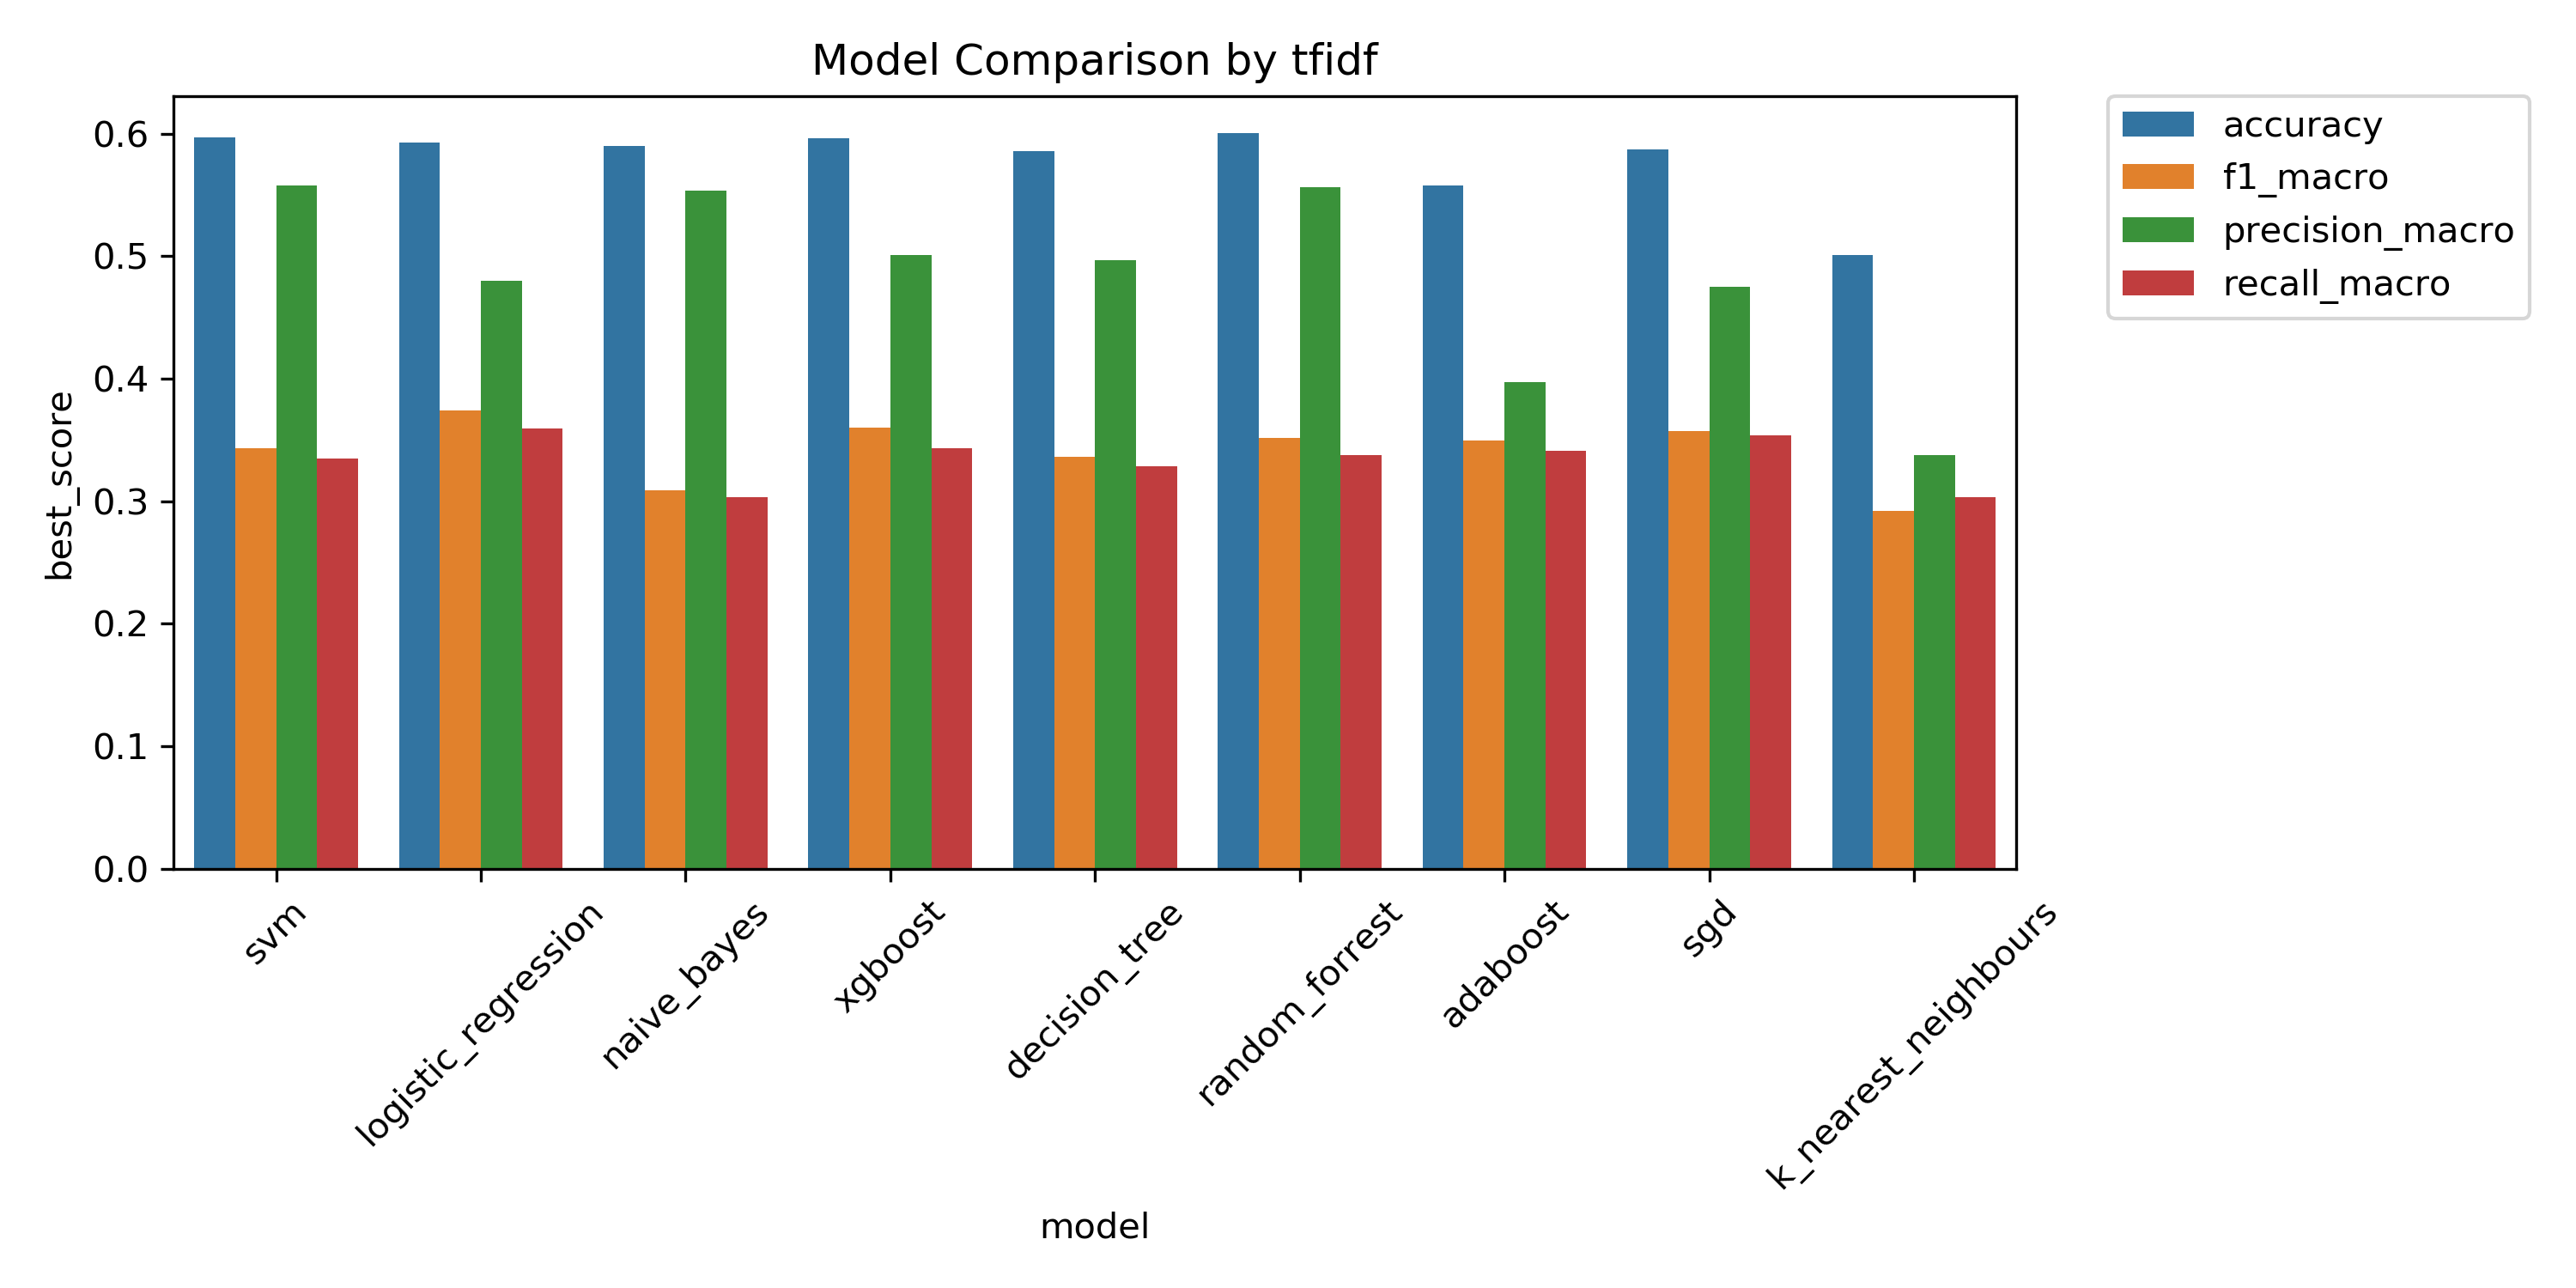
\includegraphics[scale=0.3]{figures/ns_m1tfidf}
    \label{fig:ns_m1tfidf}
}
\subfigure[Model 1 with under-sampling - CM]{
    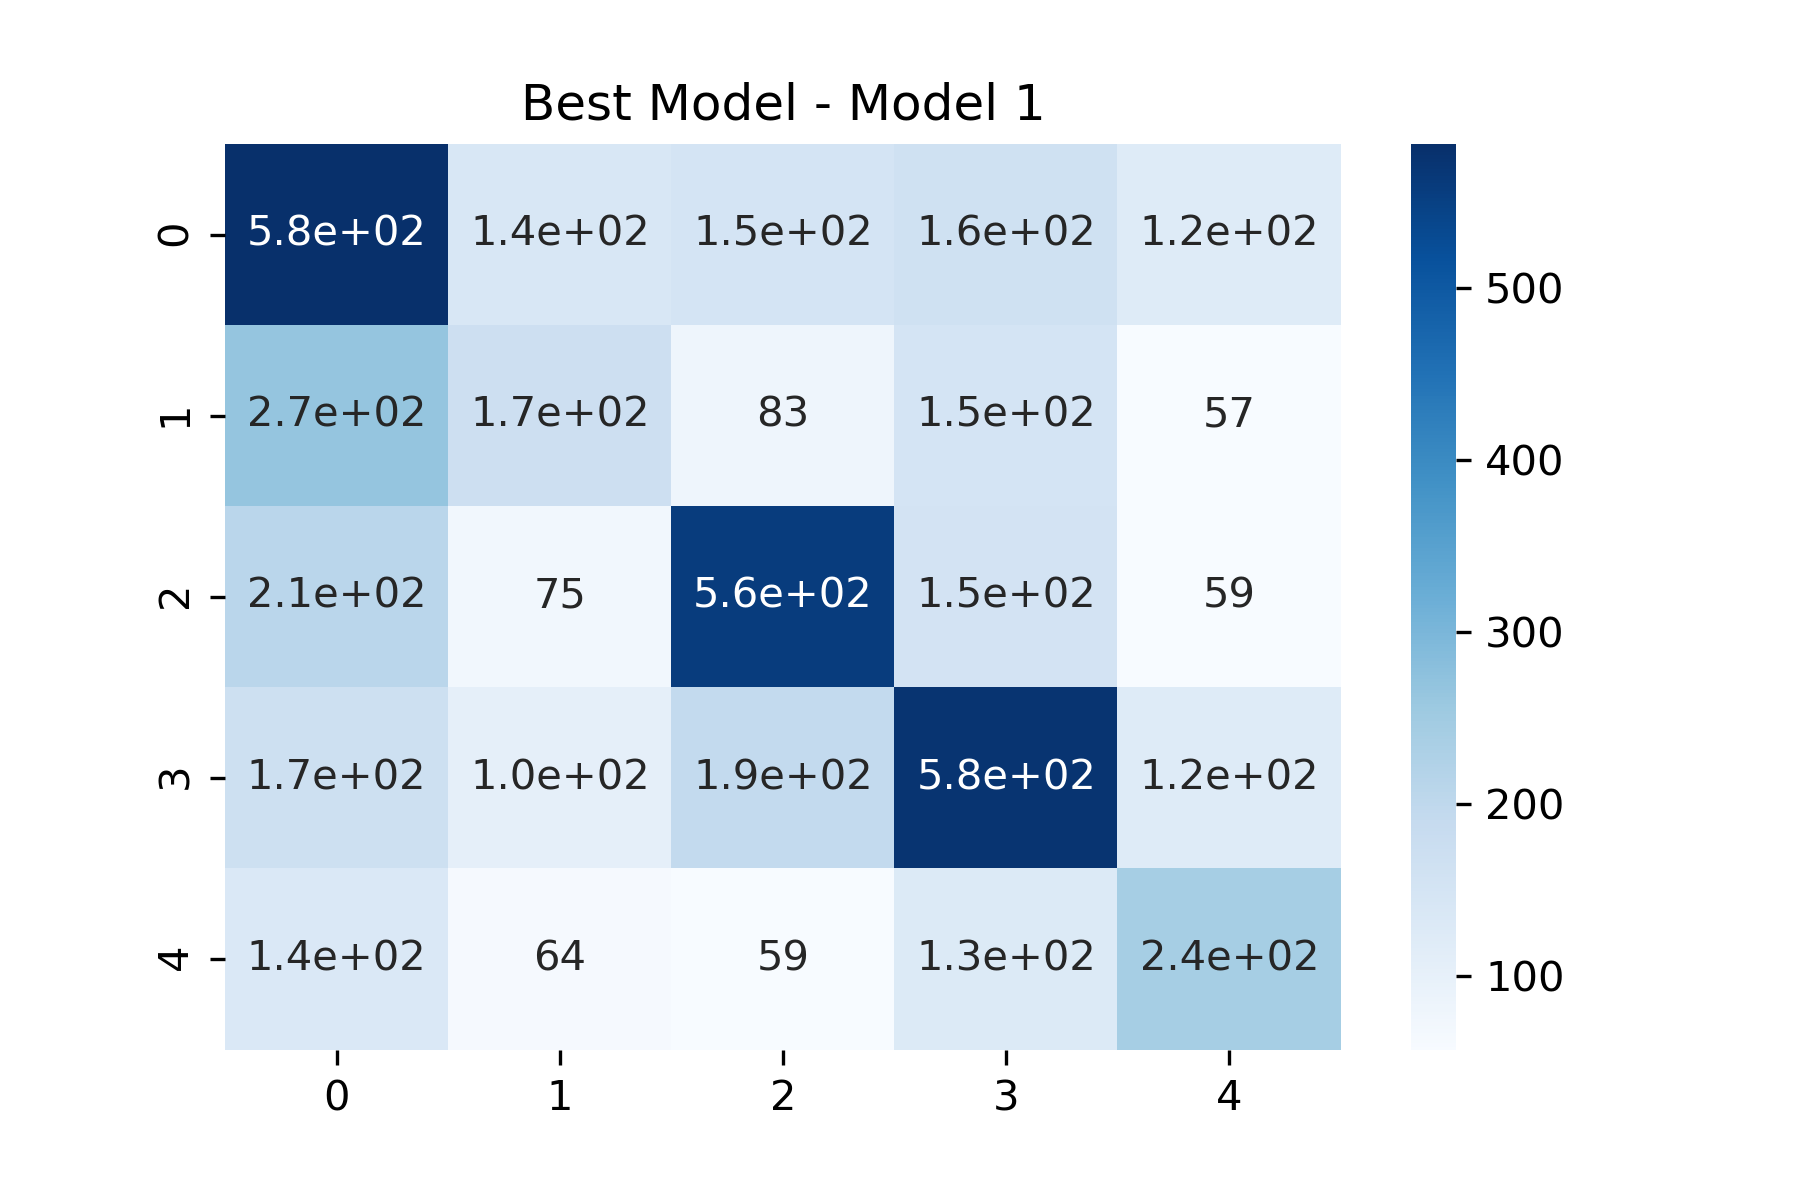
\includegraphics[scale=0.5]{figures/us_m1cm}
    \label{fig:us_m1cm}
}
\subfigure[Model 1 without under-sampling - CM]{
    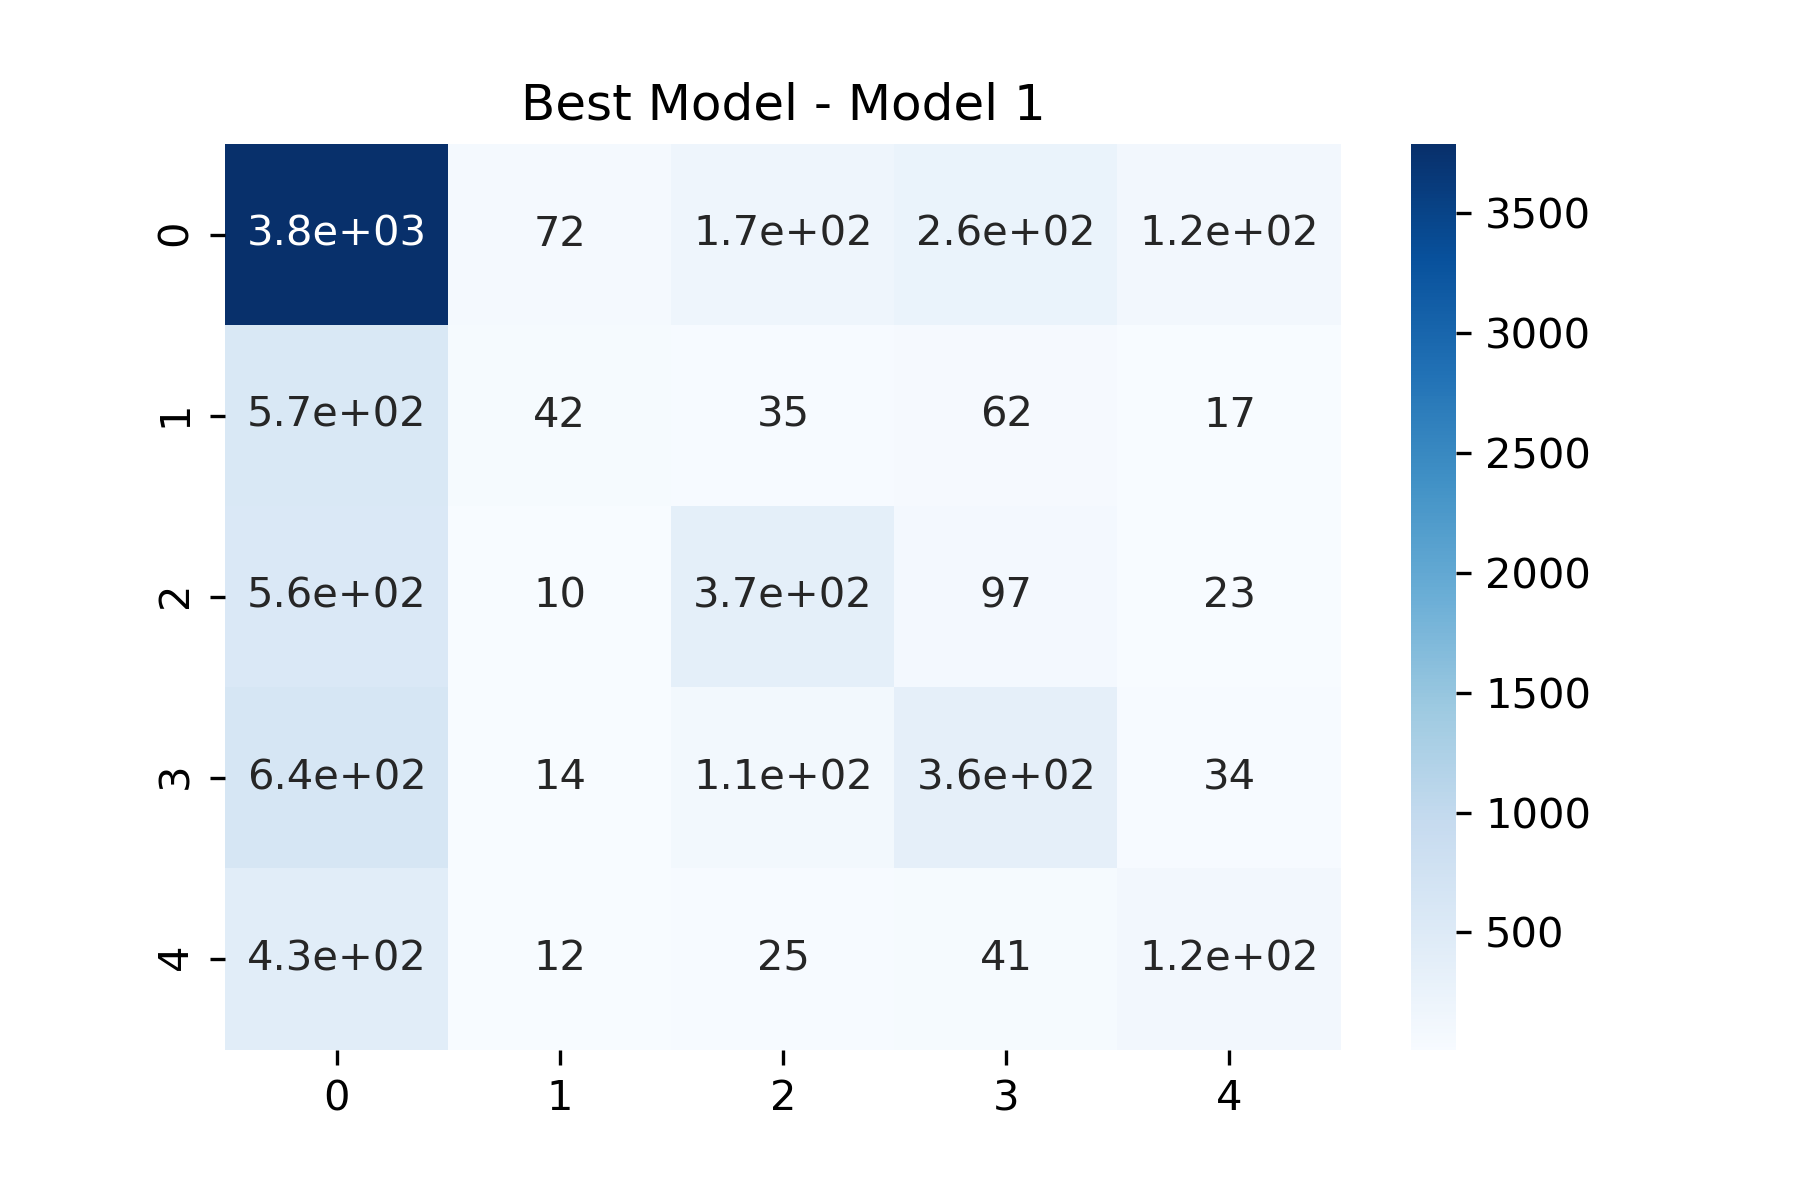
\includegraphics[scale=0.5]{figures/ns_m1cm}
    \label{fig:ns_m1cm}
}

\end{center}
\caption{Model 1 Results}
\label{fig:model1results}
\end{figure}



\begin{figure}[tbp]
\begin{center}

\subfigure[Model 2 with under-sampling - BOW]{
    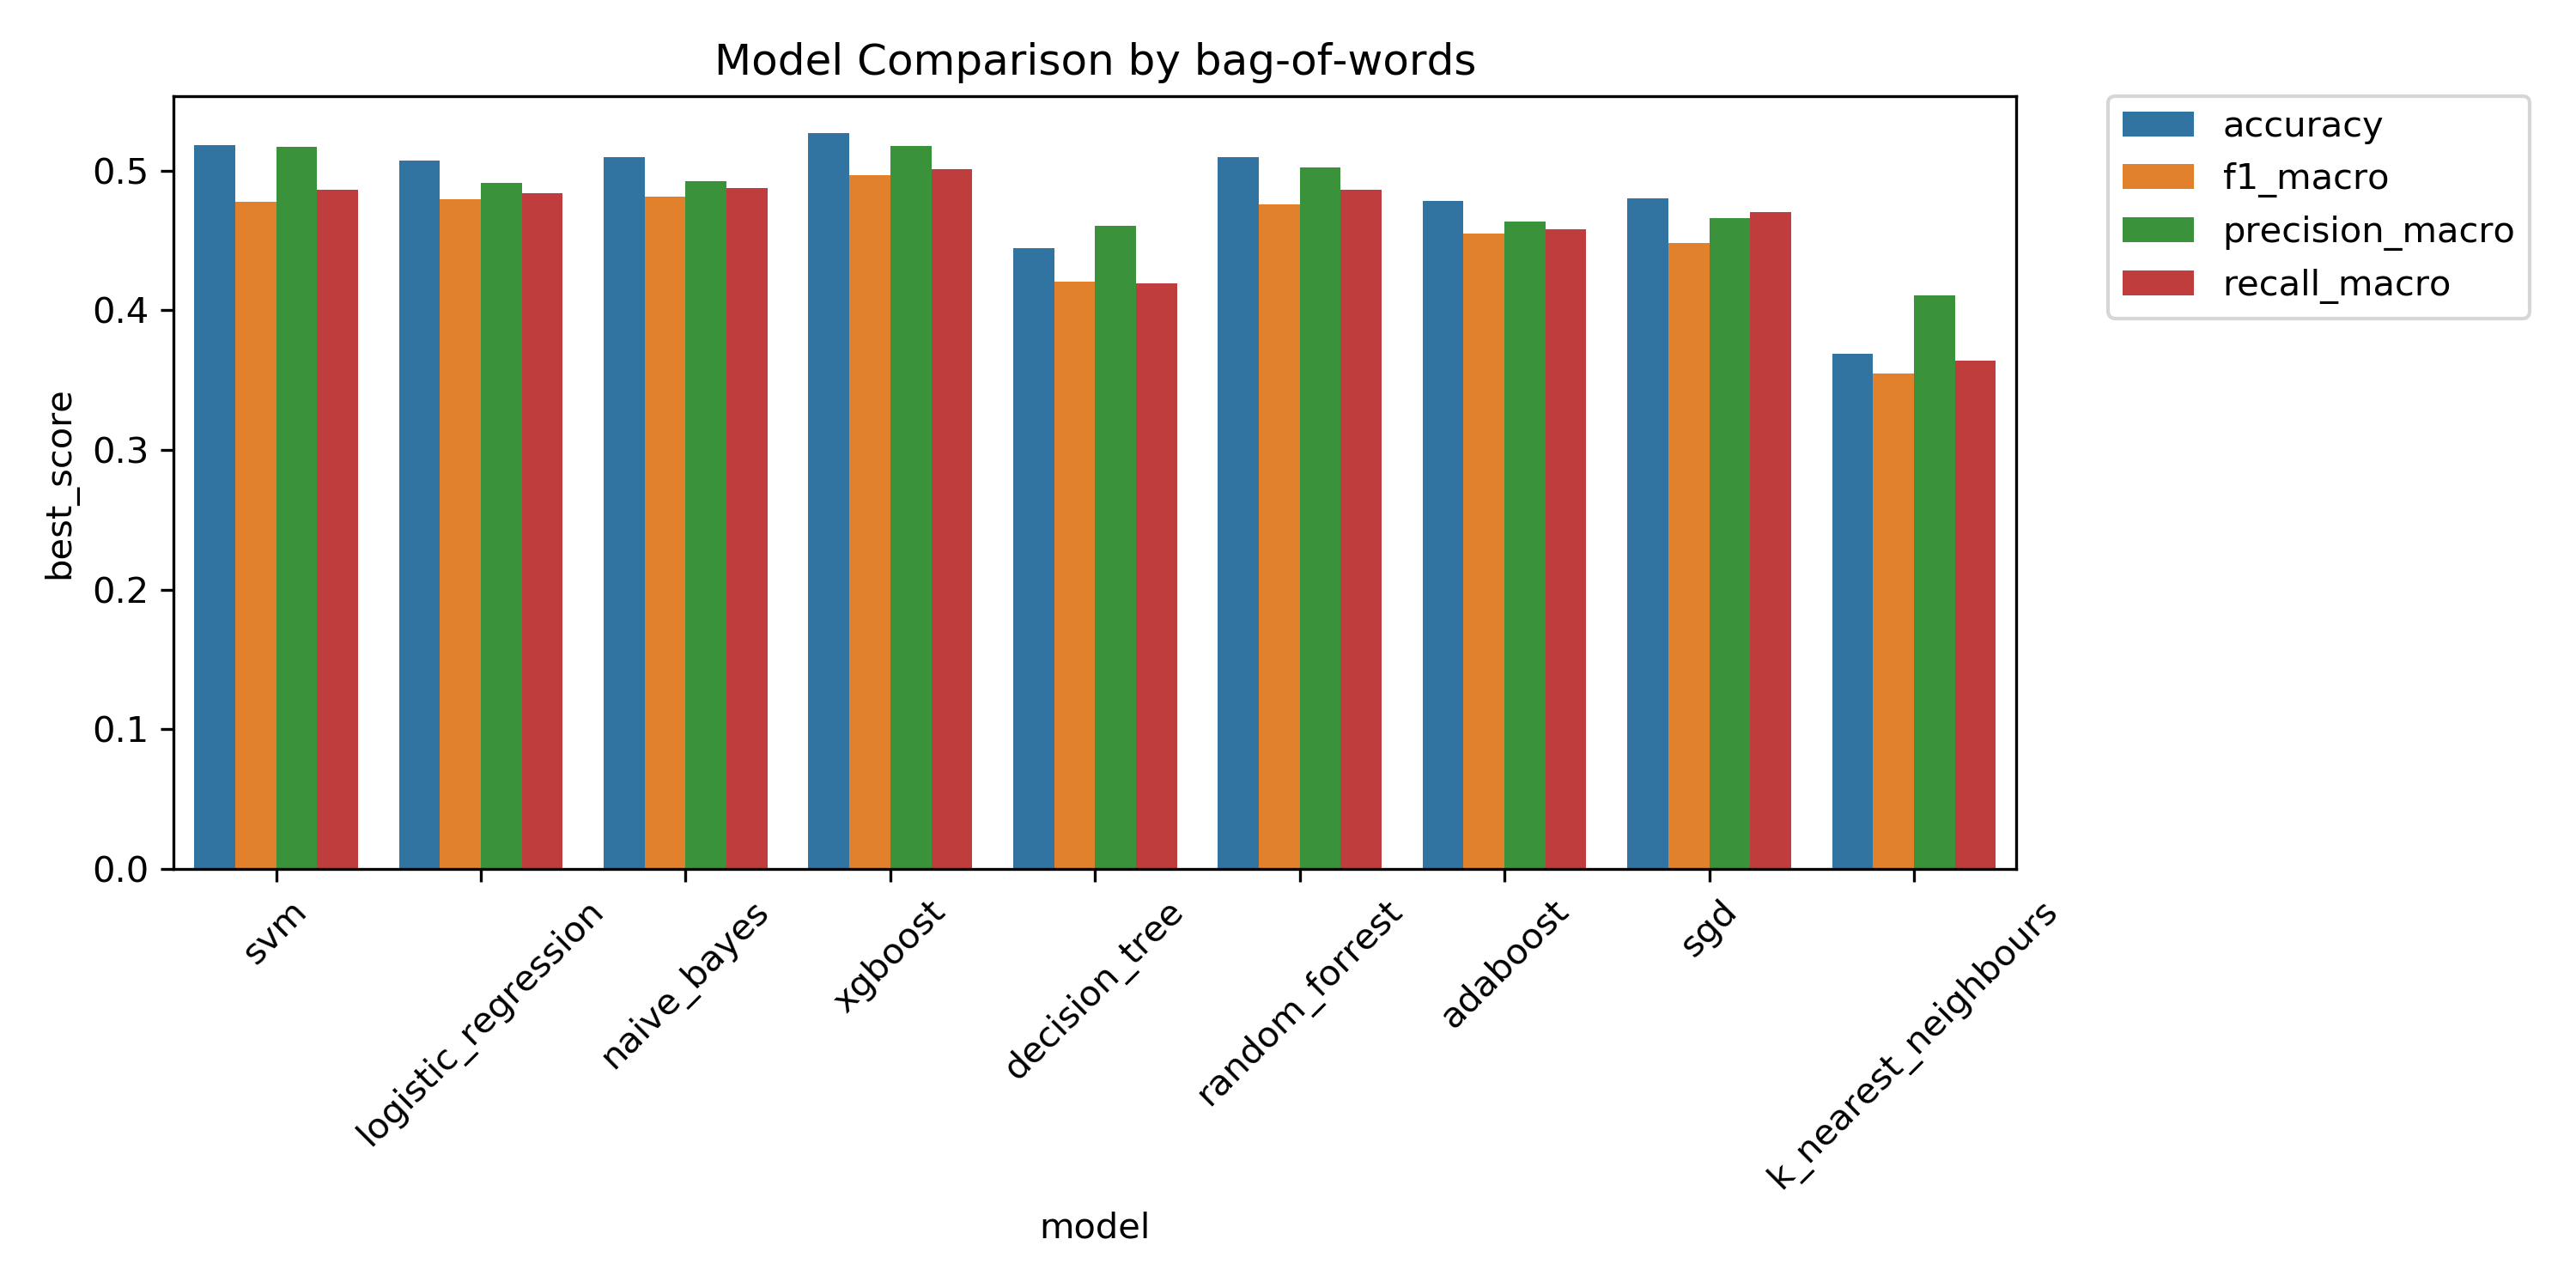
\includegraphics[scale=0.3]{figures/us_m2bow}
    \label{fig:us_m2bow}
}
\subfigure[Model 2 without under-sampling - BOW]{
    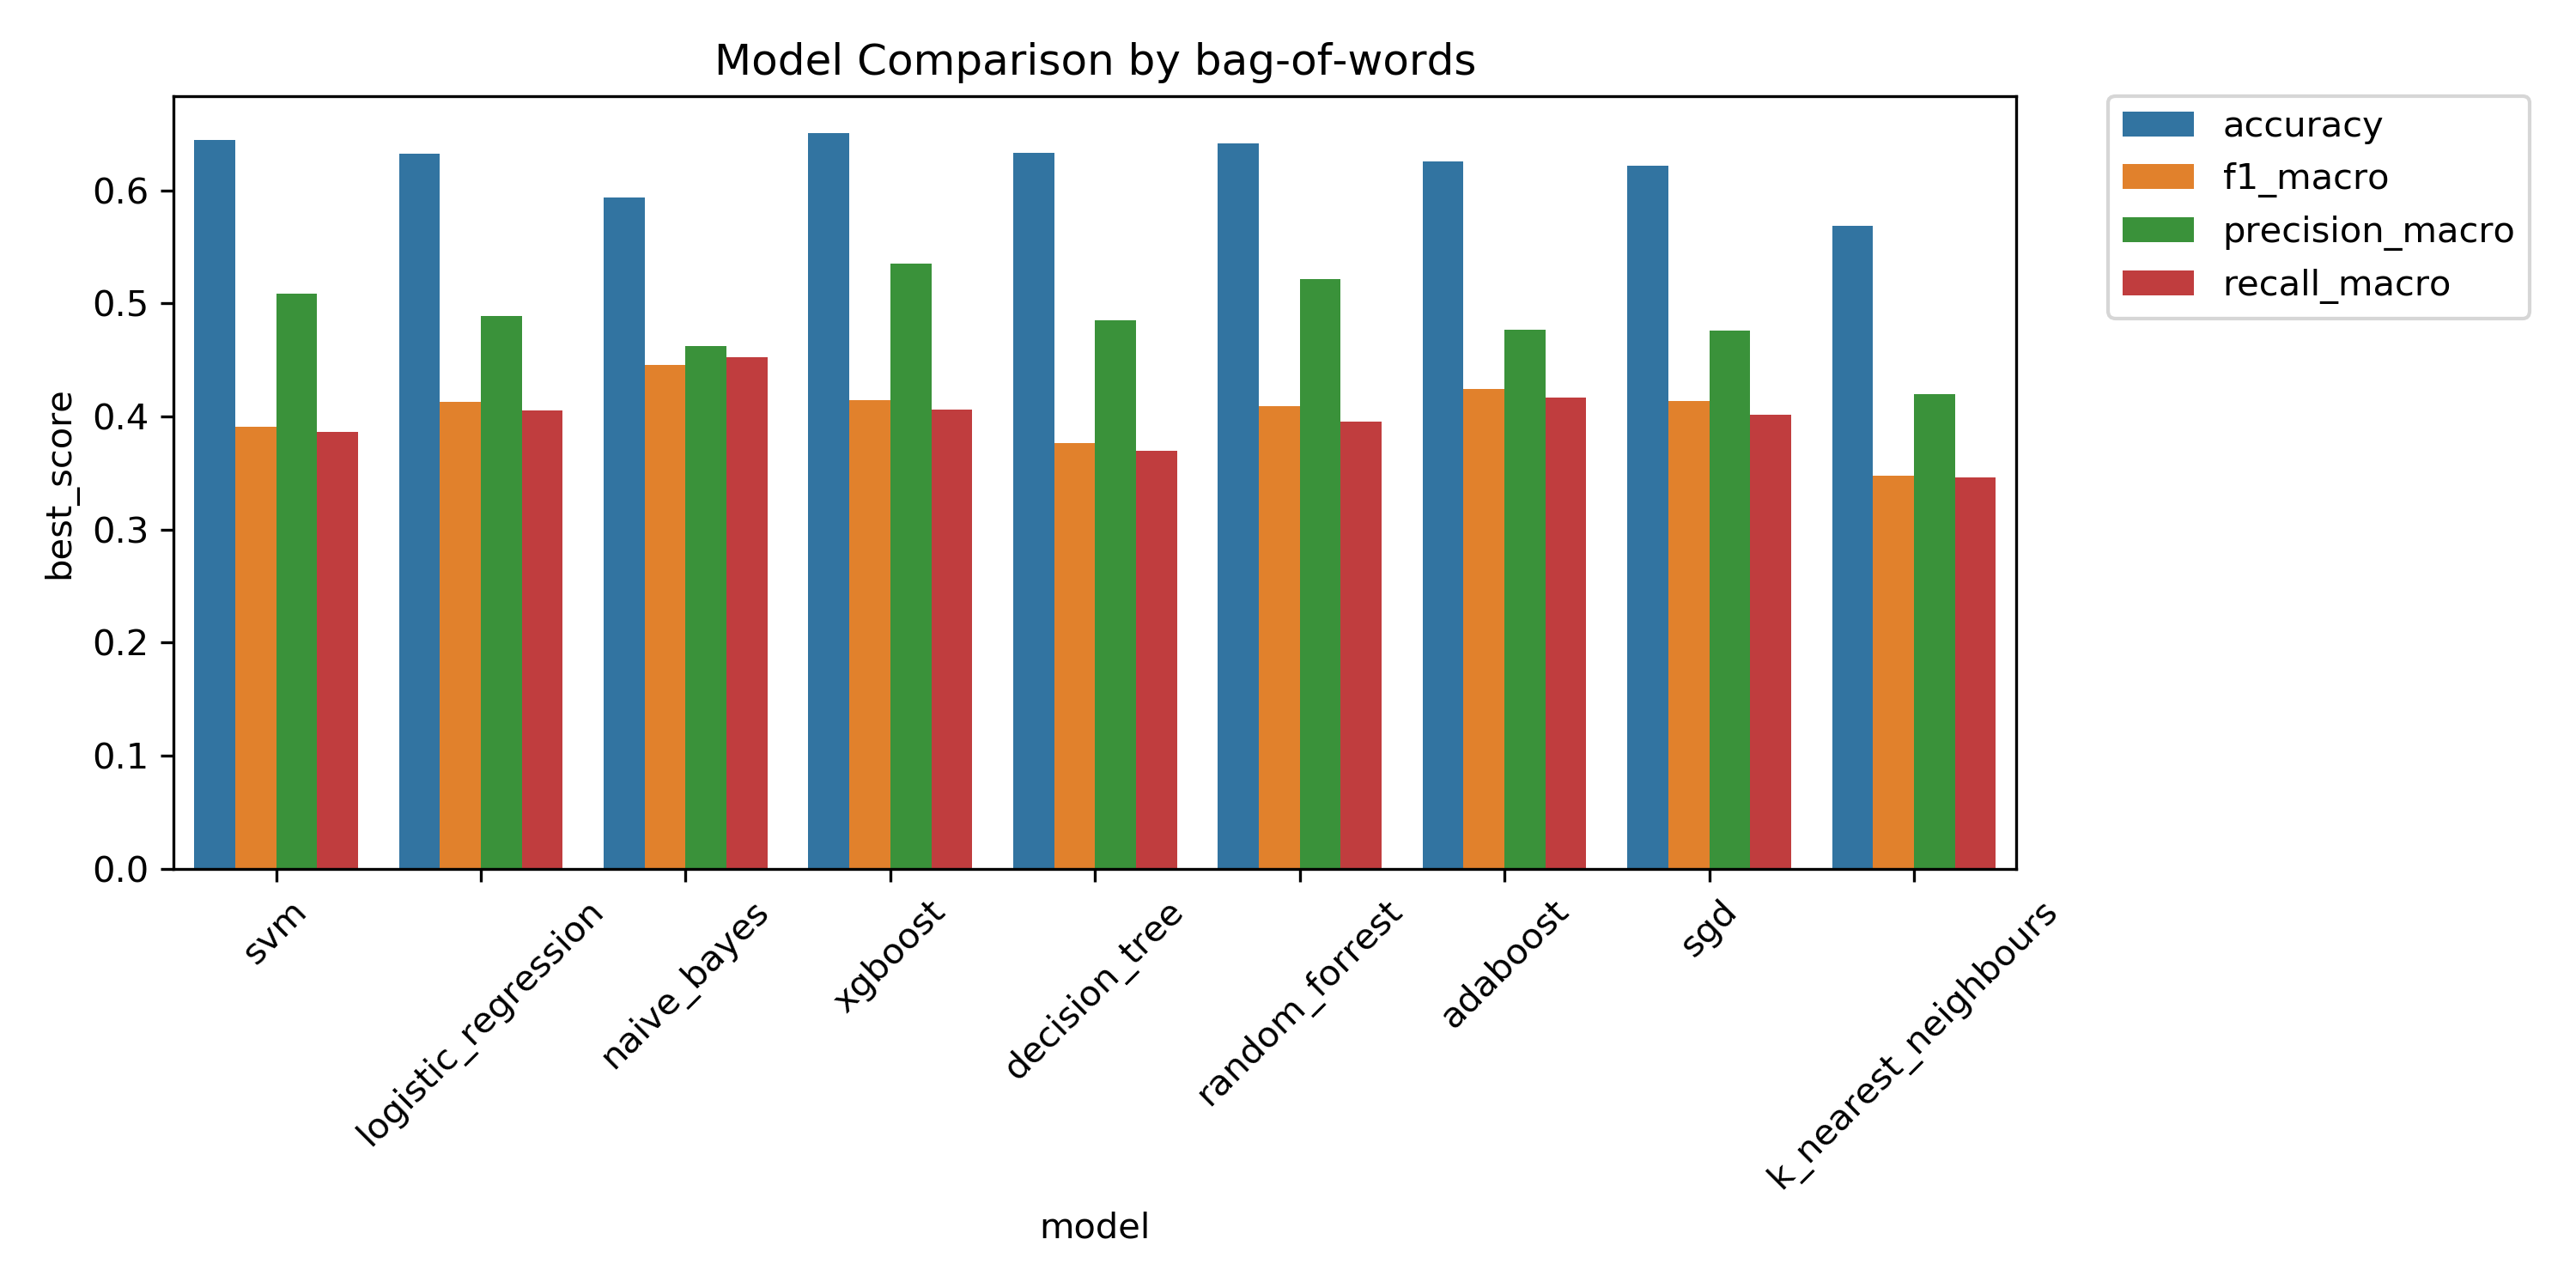
\includegraphics[scale=0.3]{figures/ns_m2bow}
    \label{fig:ns_m2bow}
}
\subfigure[Model 2 with under-sampling - TFIDF]{
    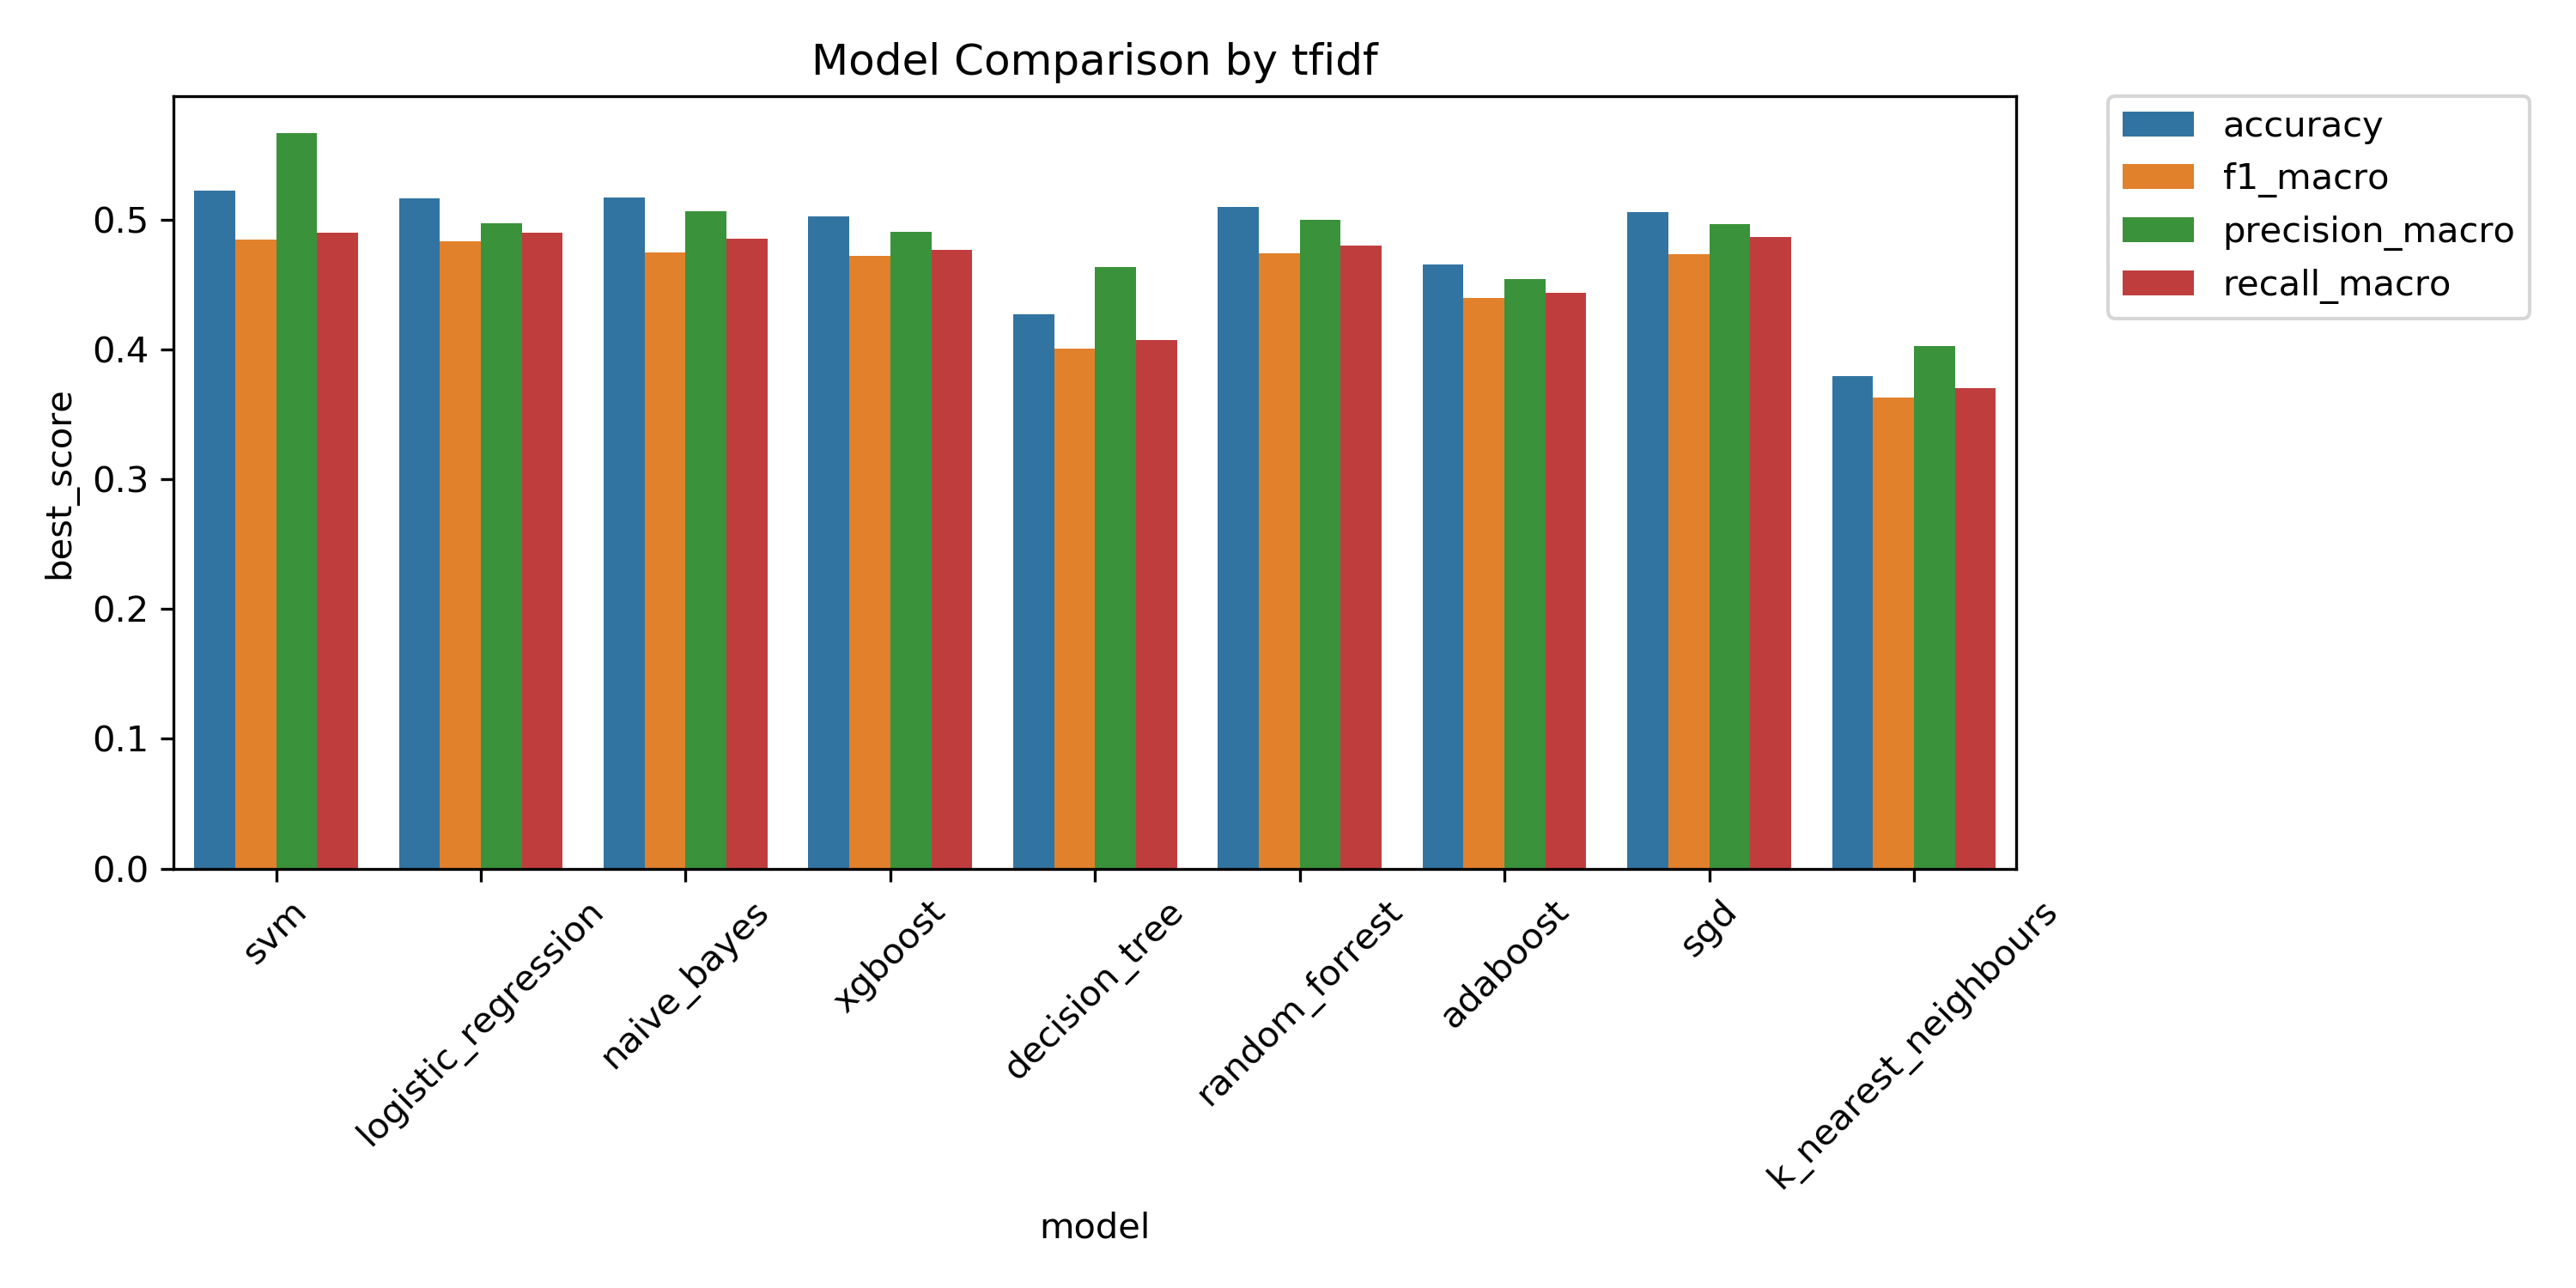
\includegraphics[scale=0.3]{figures/us_m2tfidf}
    \label{fig:us_m2tfidf}
}
\subfigure[Model 2 without under-sampling - TFIDF]{
    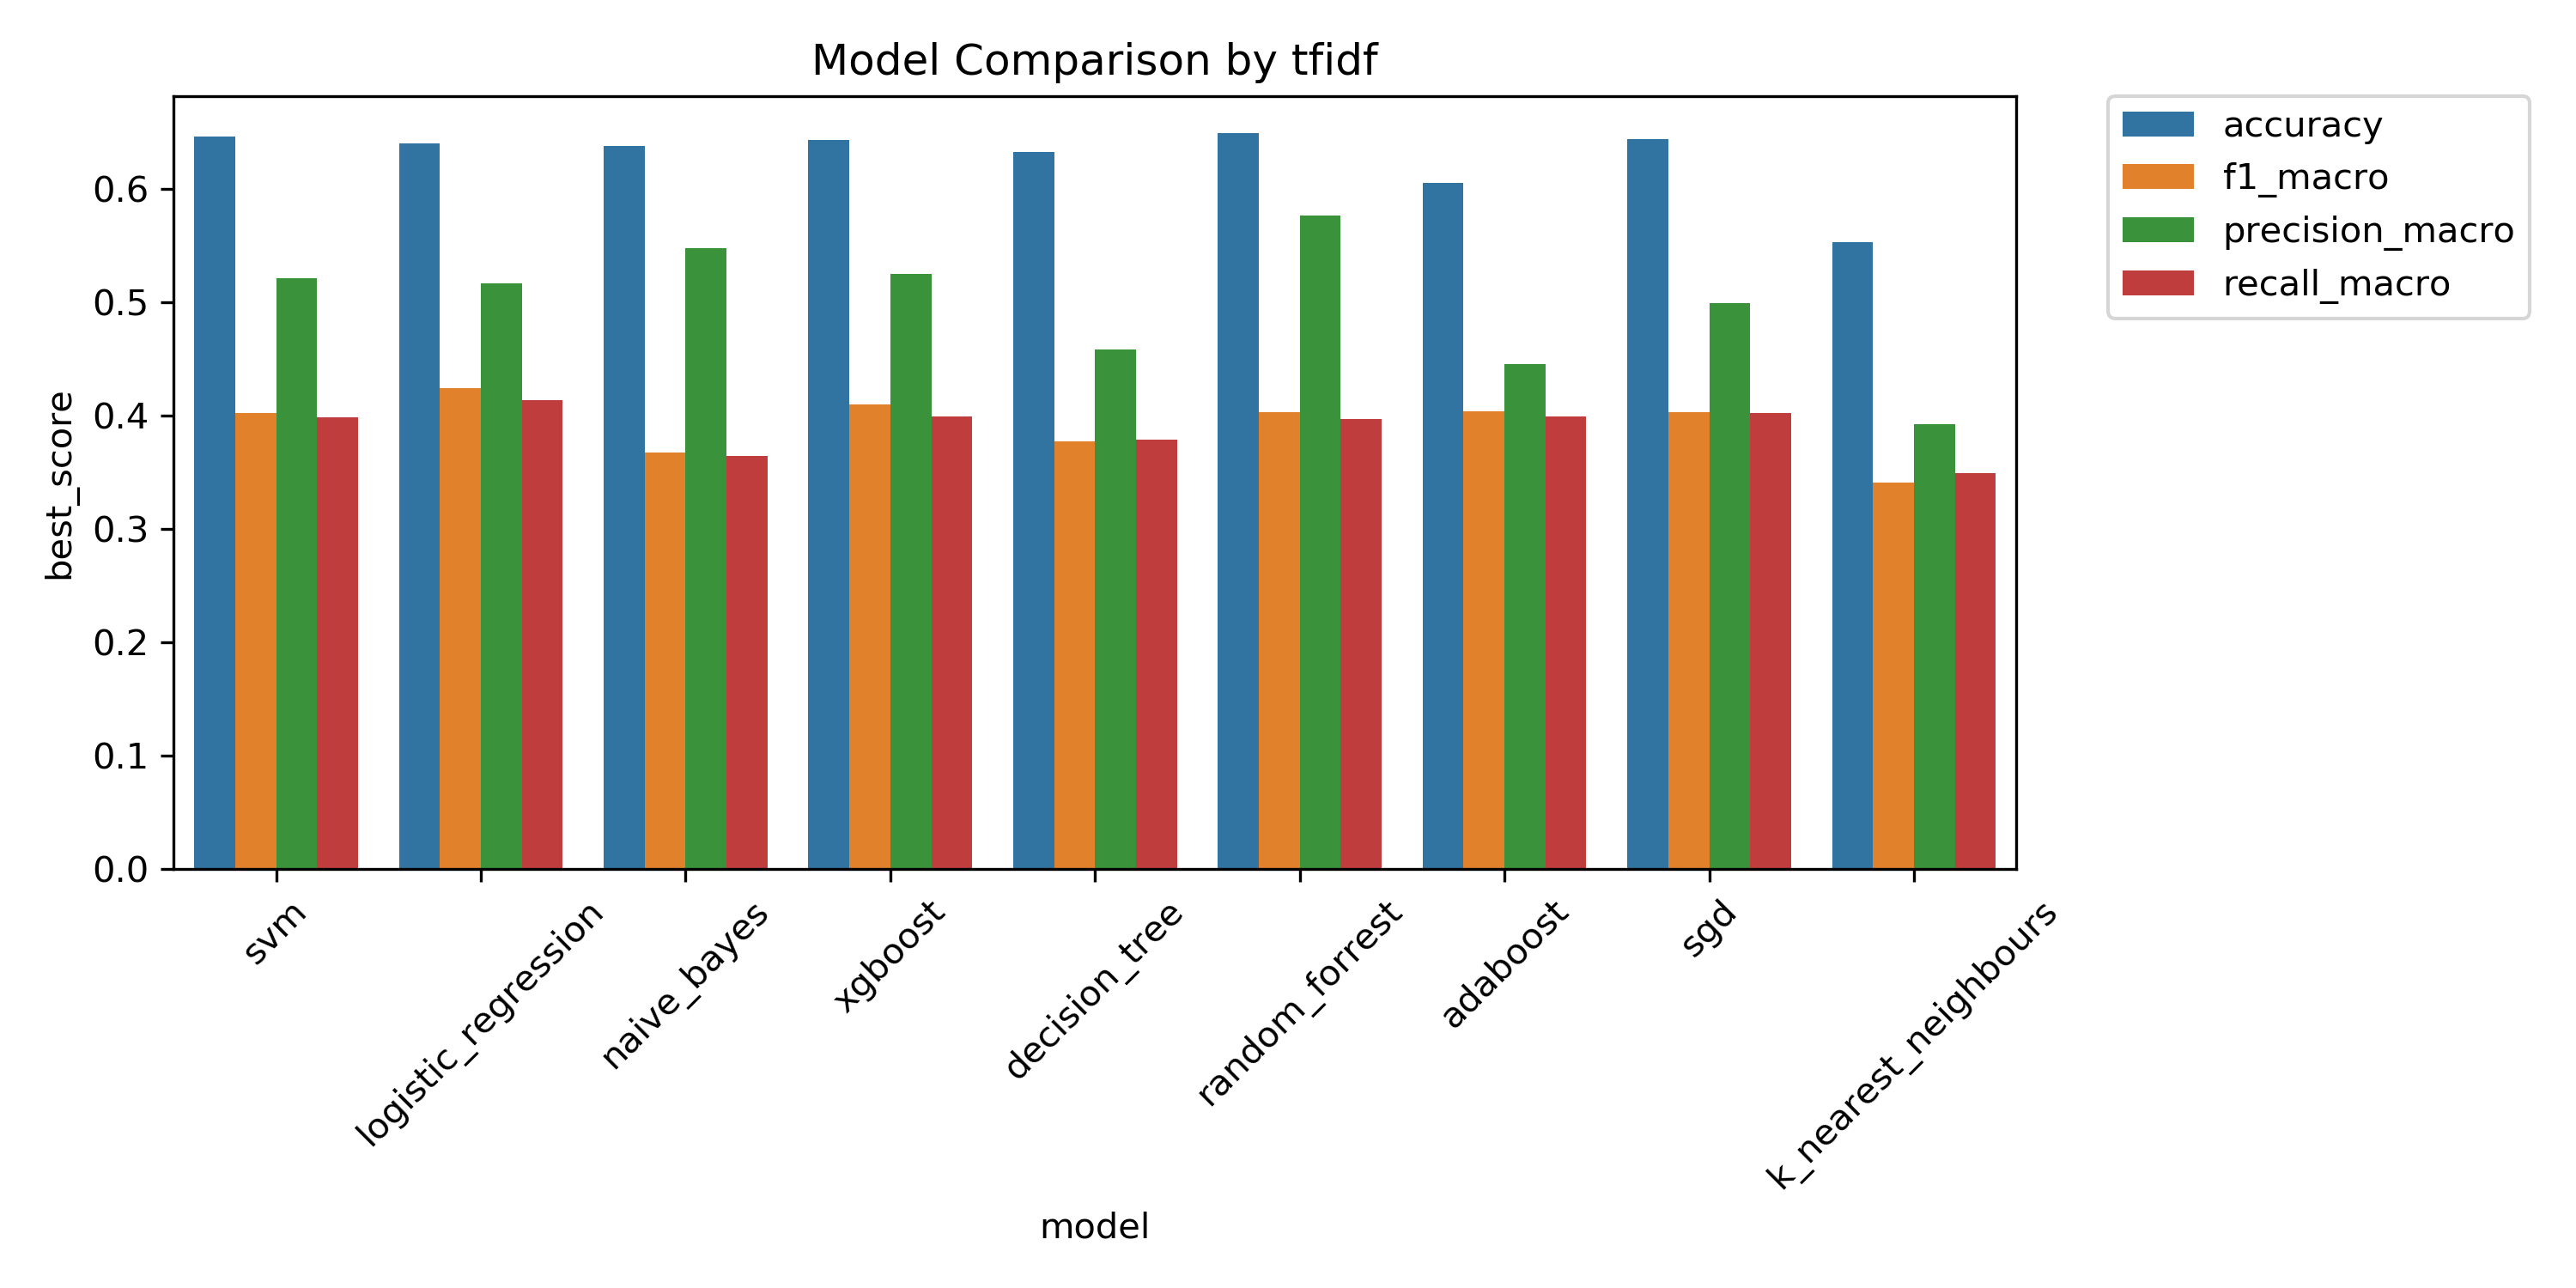
\includegraphics[scale=0.3]{figures/ns_m2tfidf}
    \label{fig:ns_m2tfidf}
}
\subfigure[Model 2 with under-sampling - CM]{
    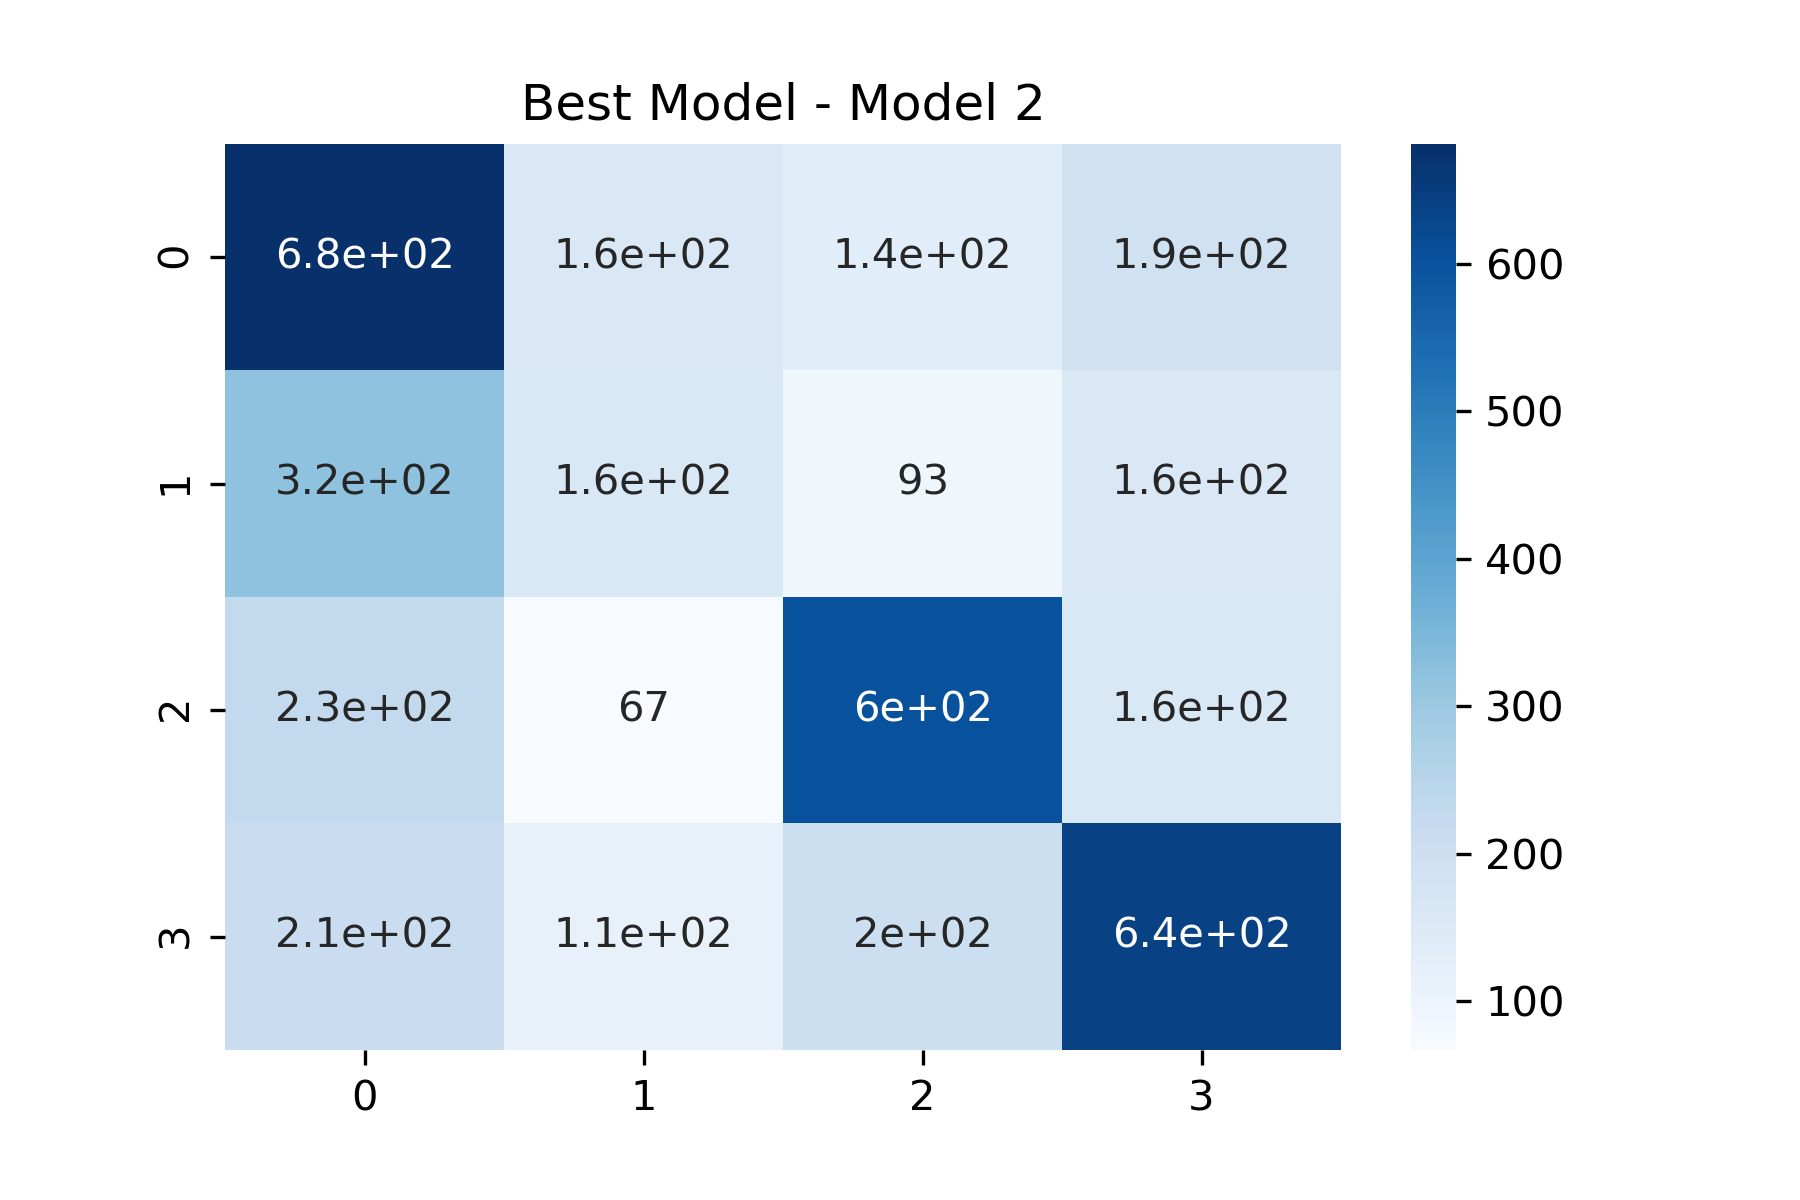
\includegraphics[scale=0.5]{figures/us_m2cm}
    \label{fig:us_m2cm}
}
\subfigure[Model 2 without under-sampling - CM]{
    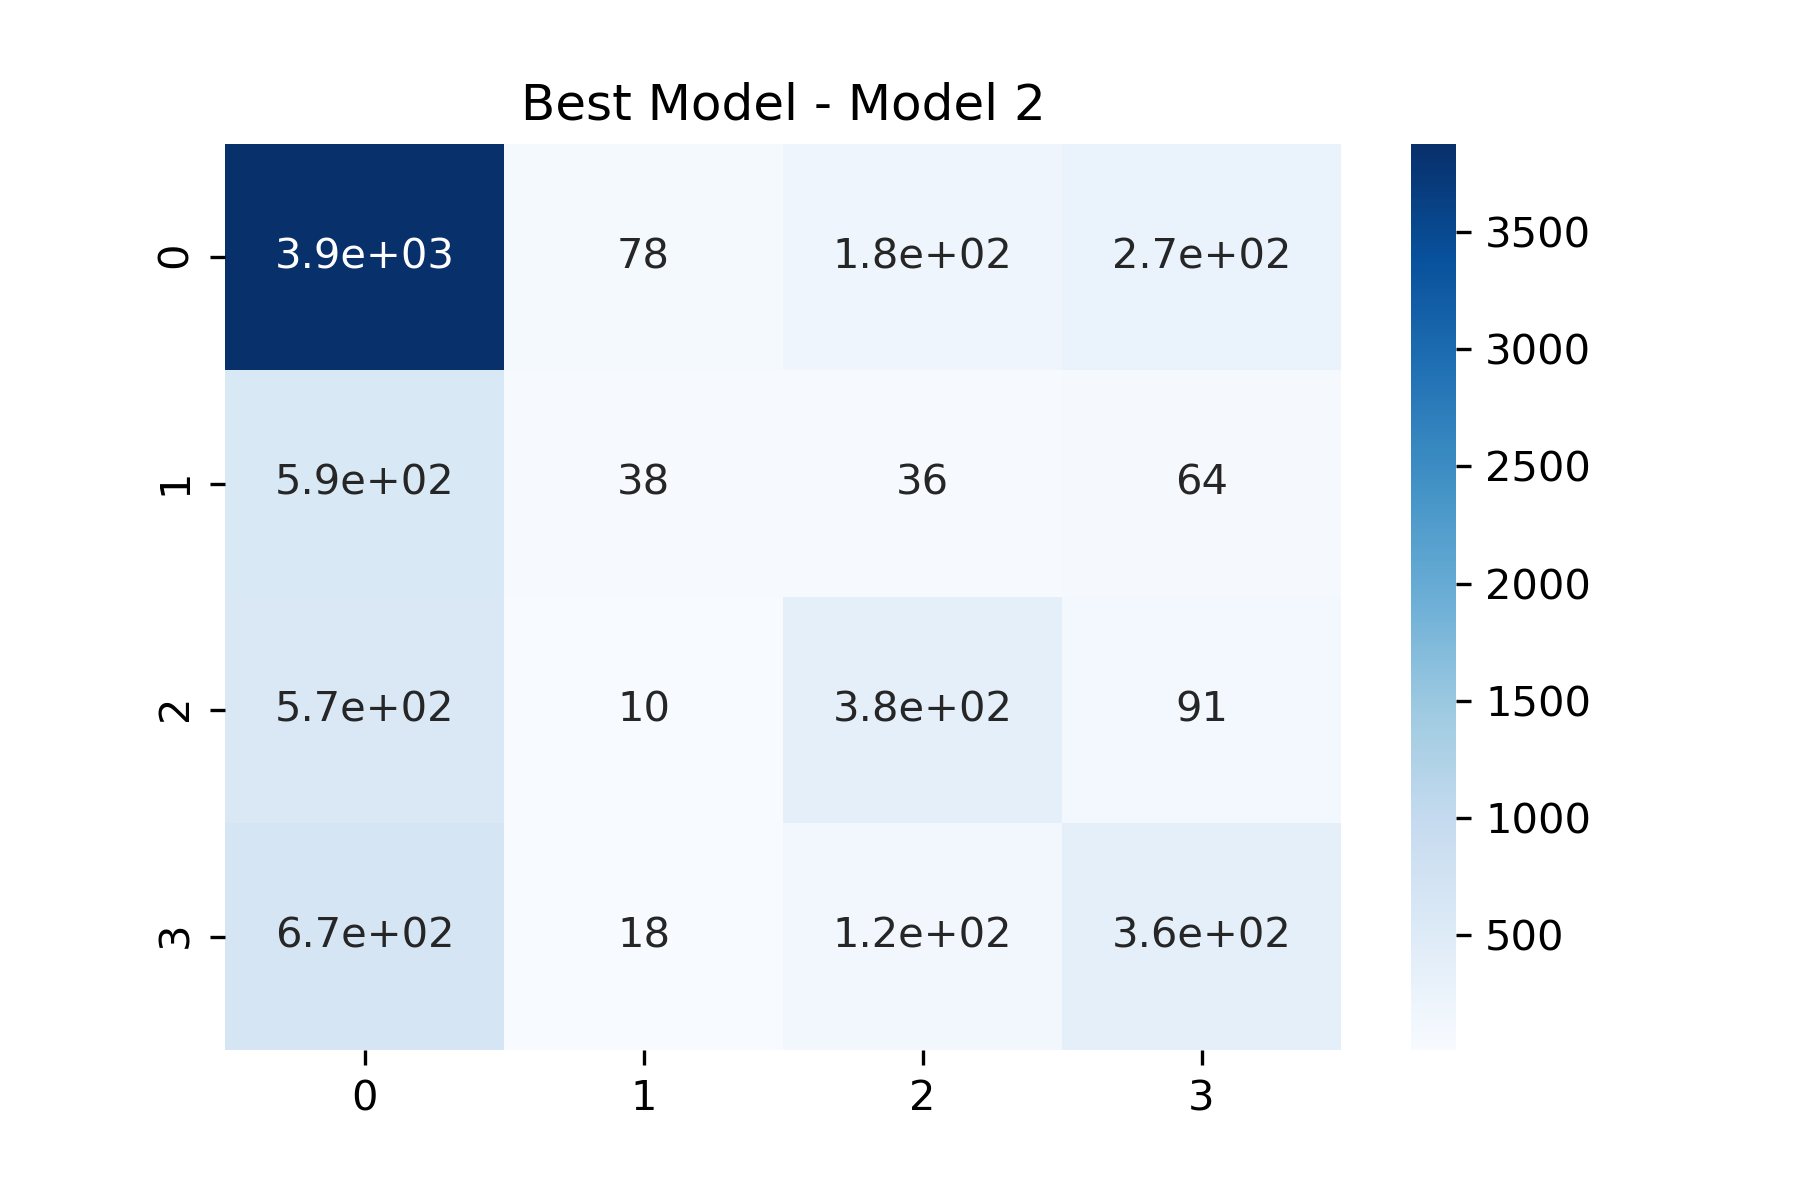
\includegraphics[scale=0.5]{figures/ns_m2cm}
    \label{fig:ns_m2cm}
}

\end{center}
\caption{Model 2 Results}
\label{fig:model2results}
\end{figure}






\begin{figure}[tbp]
\begin{center}

\subfigure[Model 3 with under-sampling - BOW]{
    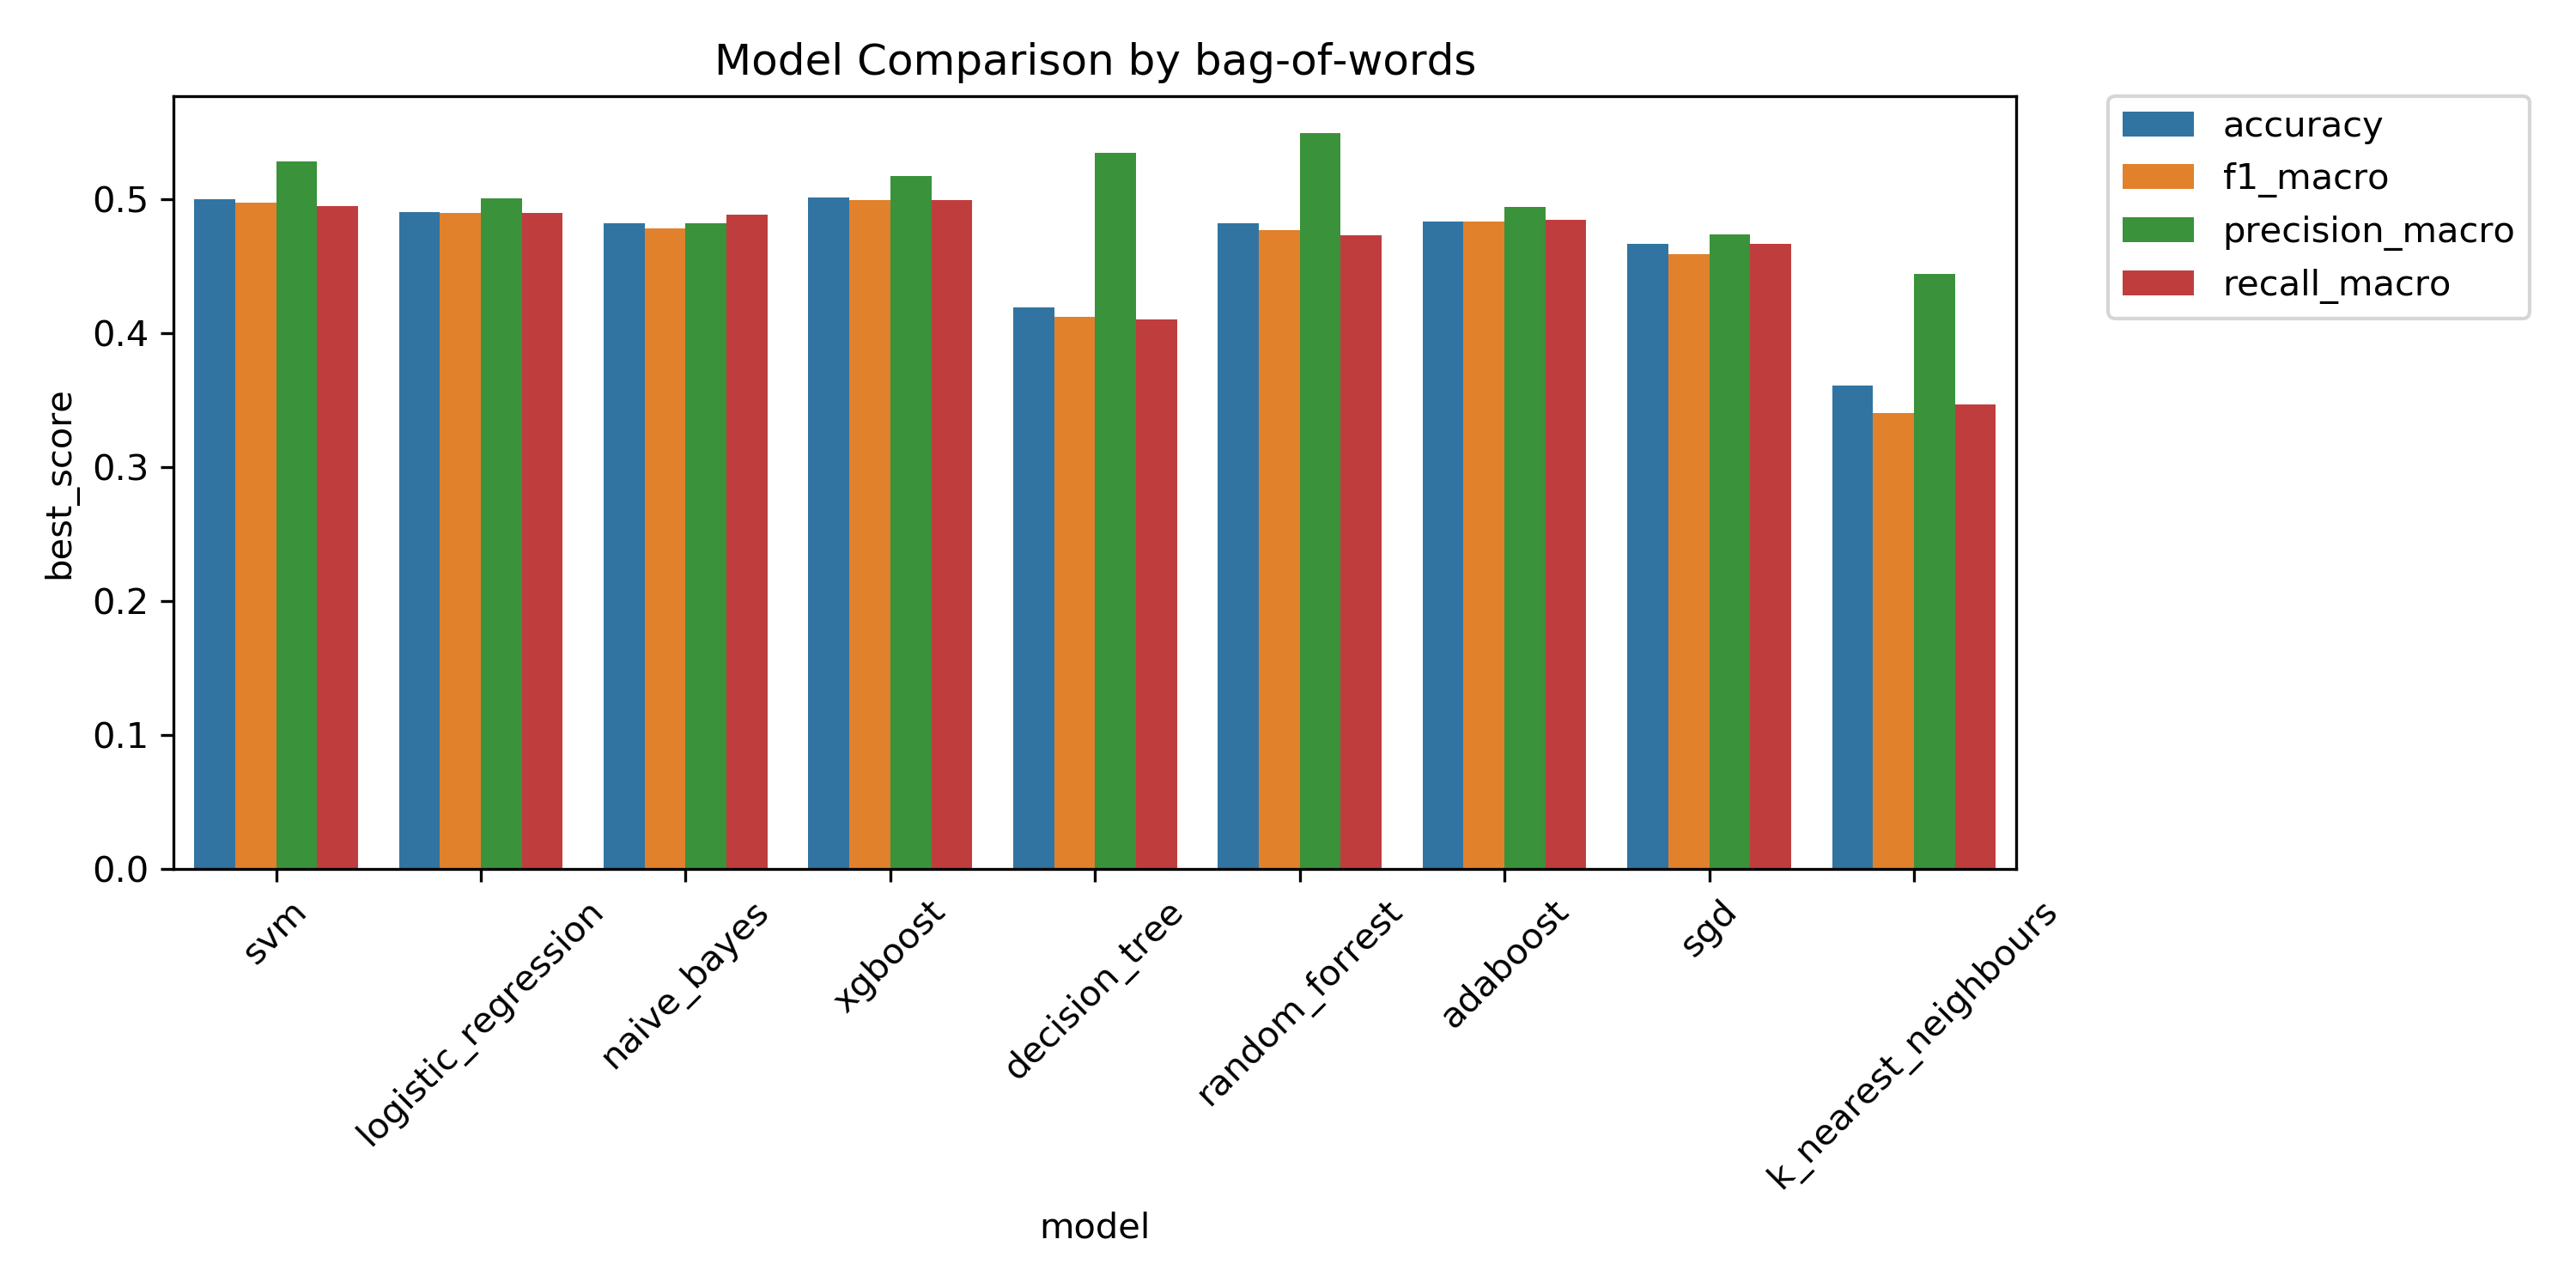
\includegraphics[scale=0.3]{figures/us_m3bow}
    \label{fig:us_m3bow}
}
\subfigure[Model 3 without under-sampling - BOW]{
    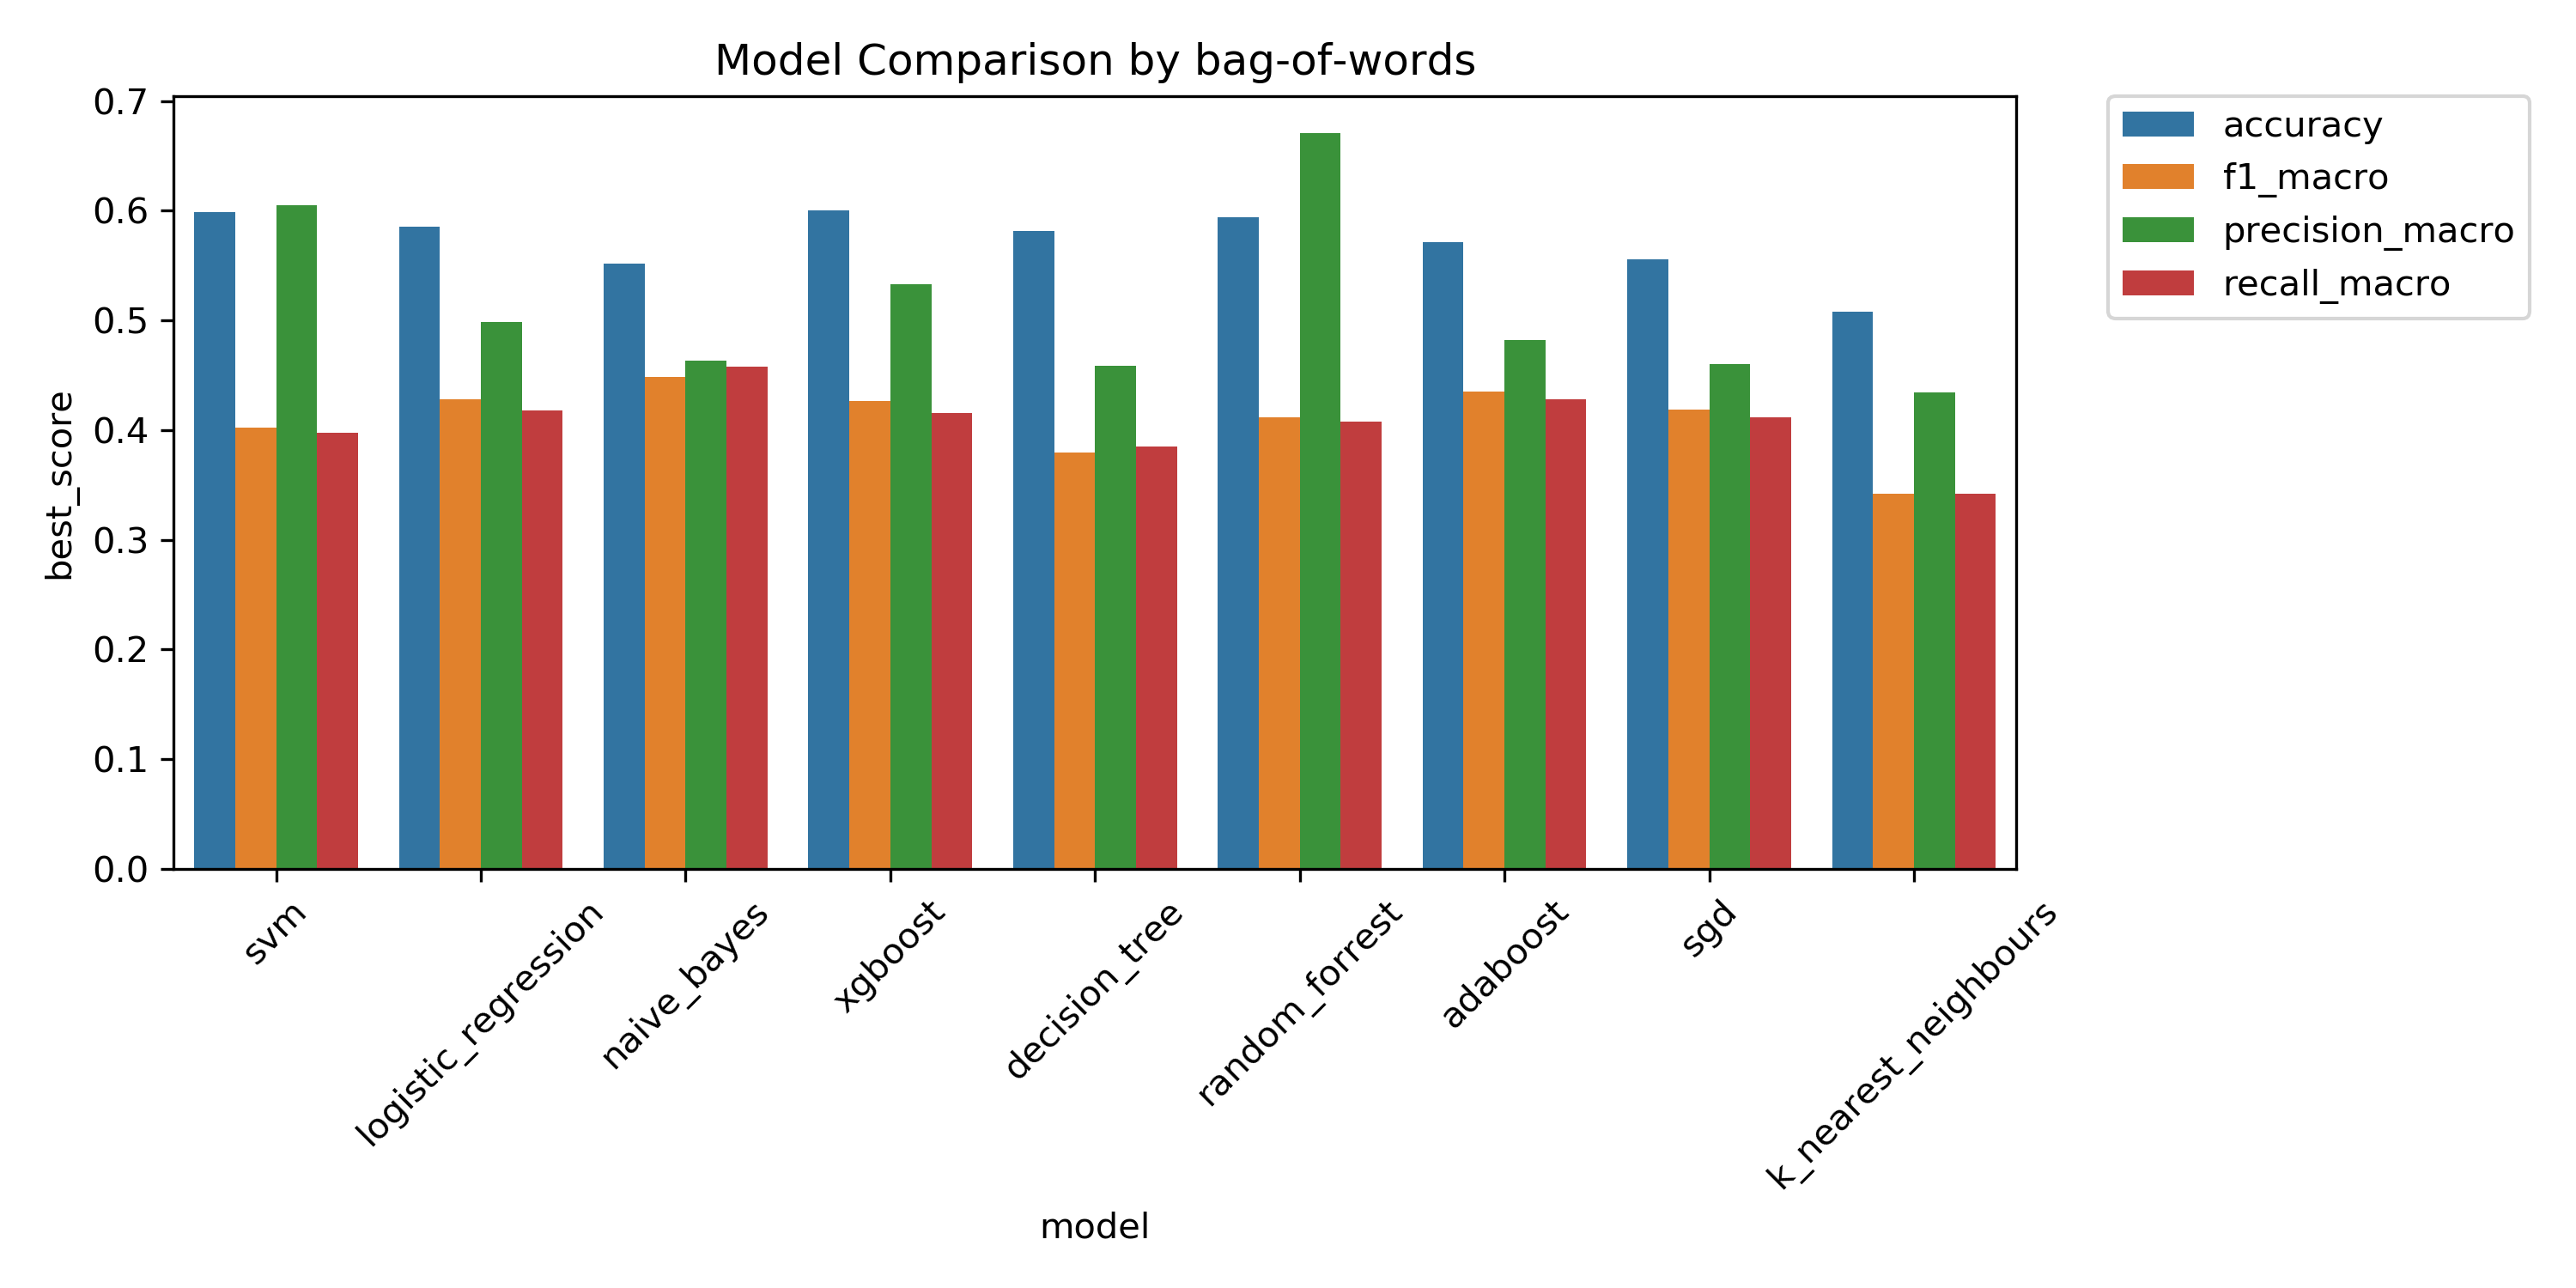
\includegraphics[scale=0.3]{figures/ns_m3bow}
    \label{fig:ns_m3bow}
}
\subfigure[Model 3 with under-sampling - TFIDF]{
    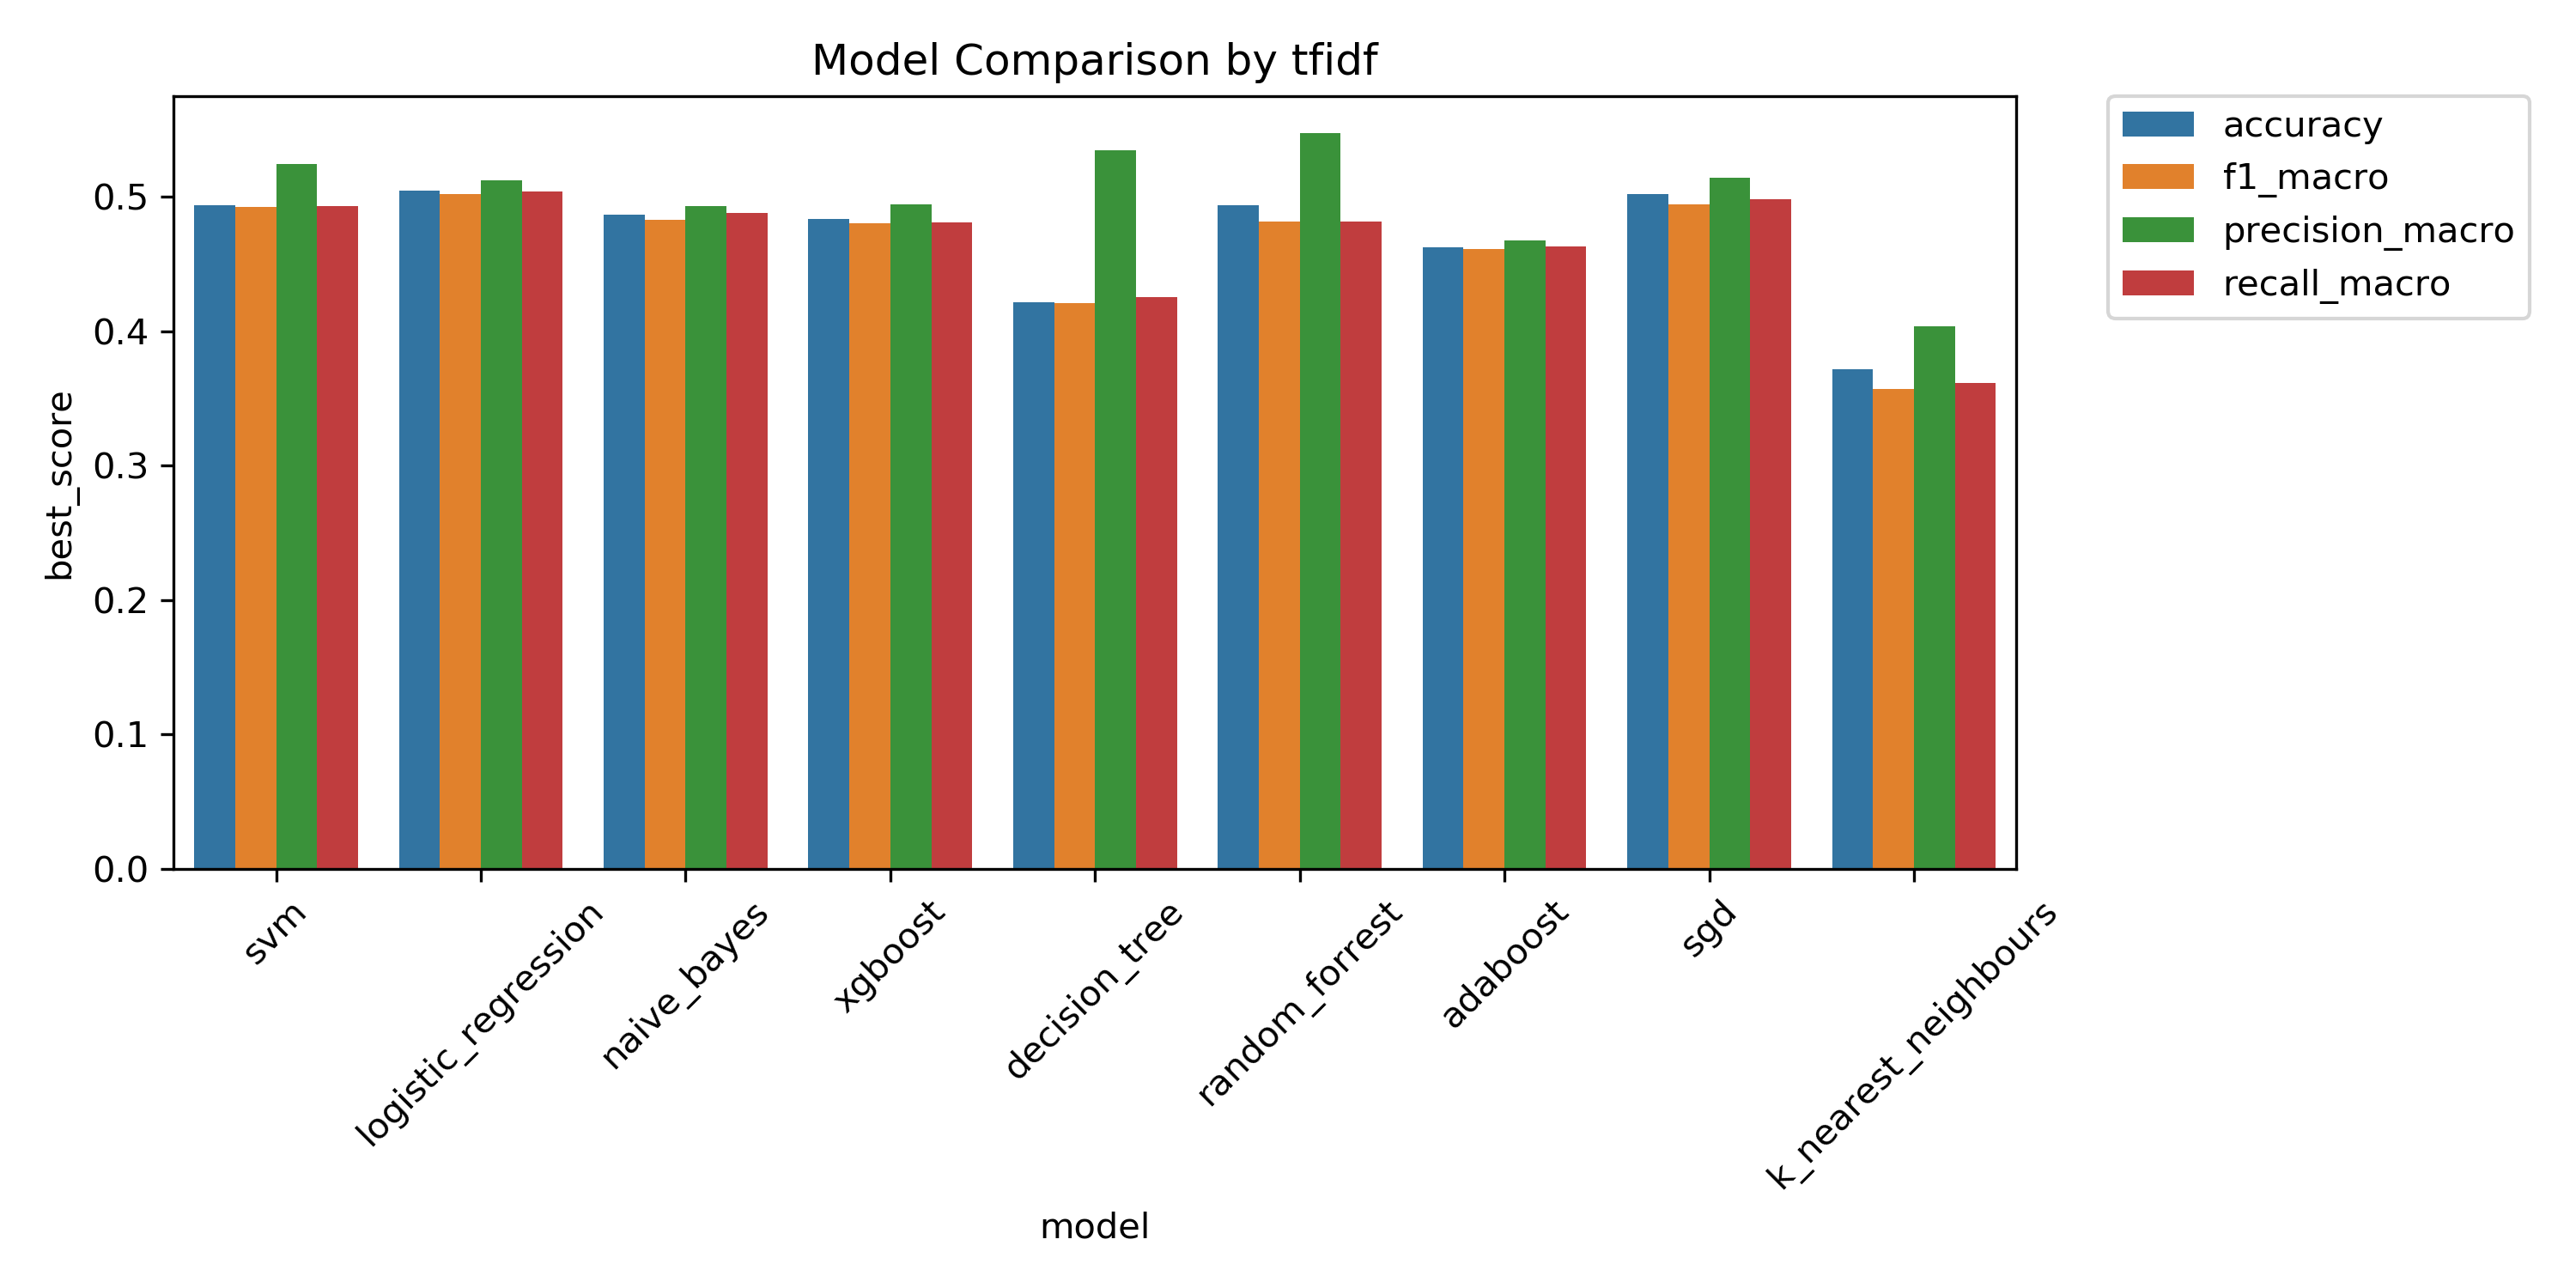
\includegraphics[scale=0.3]{figures/us_m3tfidf}
    \label{fig:us_m3tfidf}
}
\subfigure[Model 3 without under-sampling - TFIDF]{
    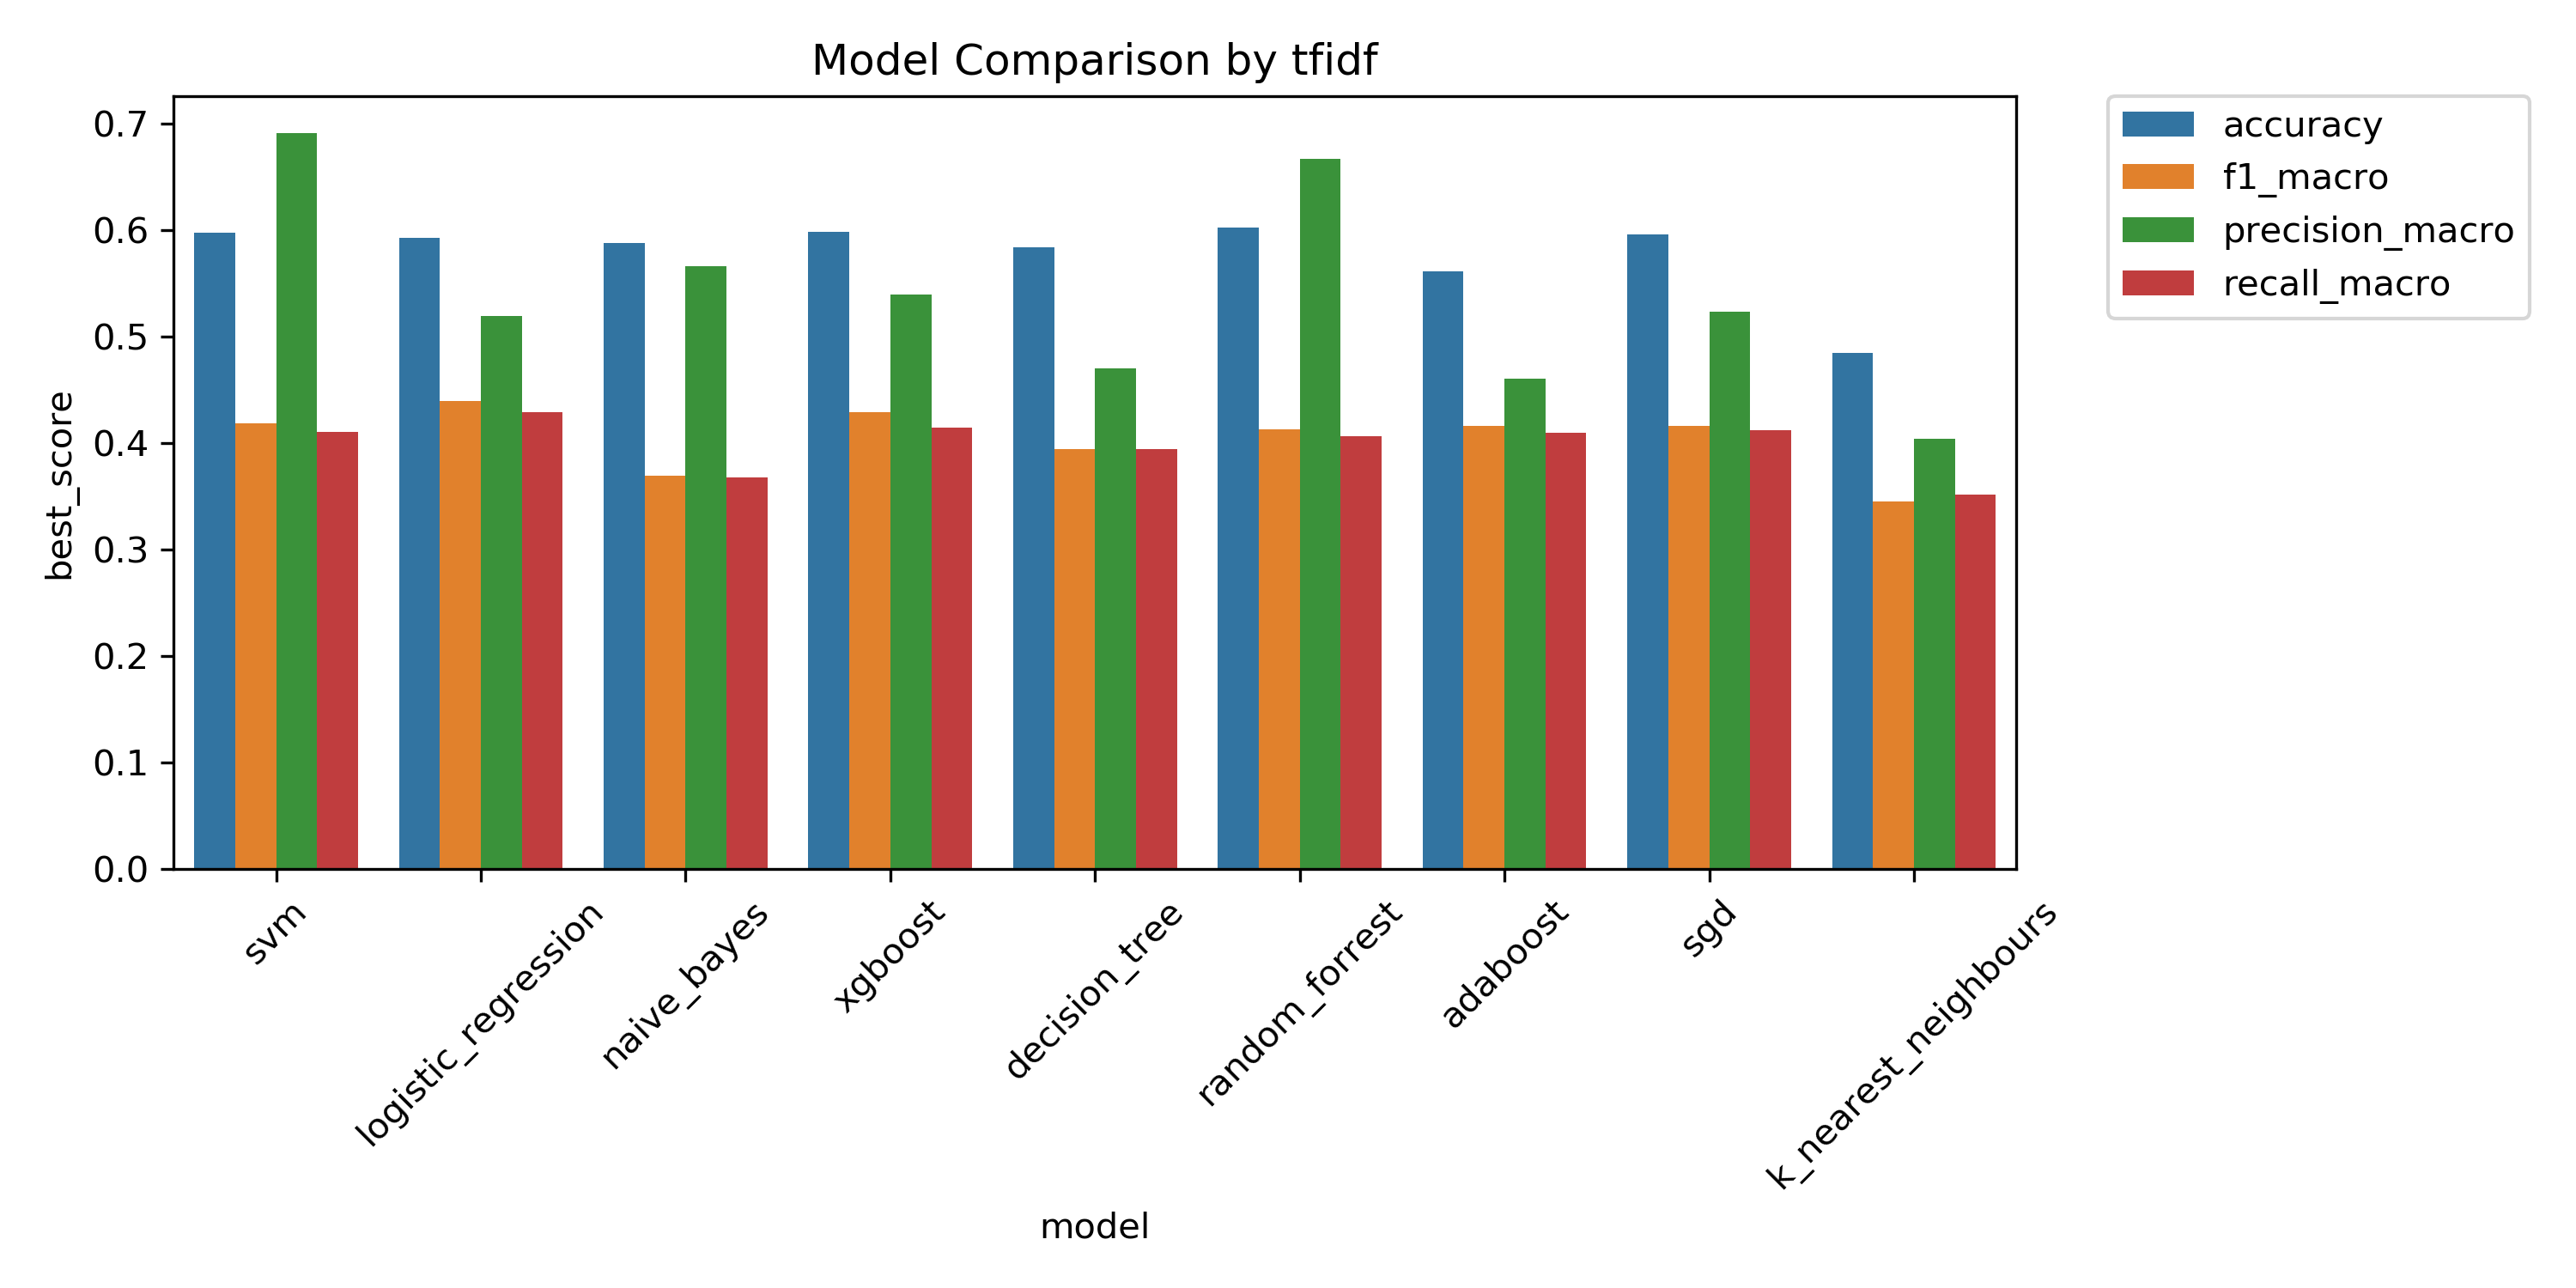
\includegraphics[scale=0.3]{figures/ns_m3tfidf}
    \label{fig:ns_m2tfidf}
}
\subfigure[Model 3 with under-sampling - CM]{
    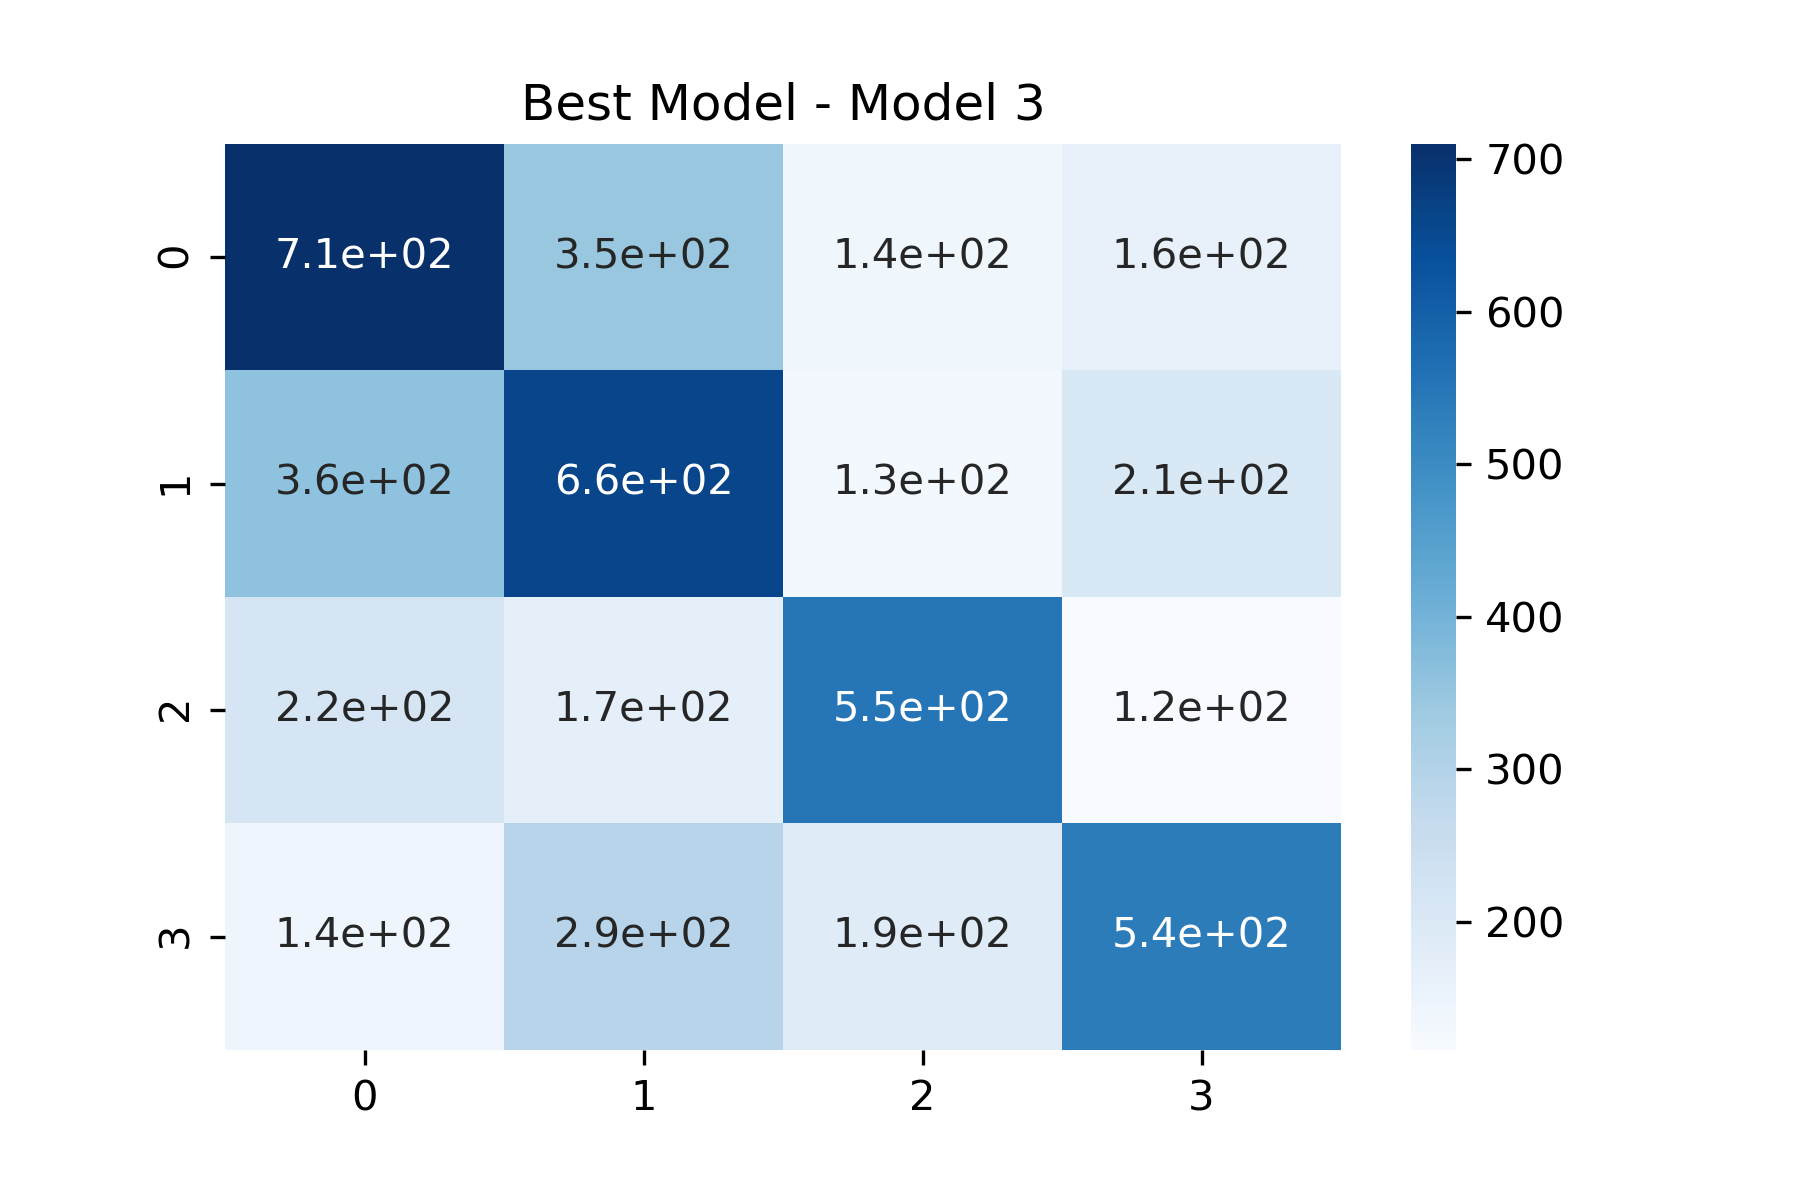
\includegraphics[scale=0.5]{figures/us_m3cm}
    \label{fig:us_m3cm}
}
\subfigure[Model 3 without under-sampling - CM]{
    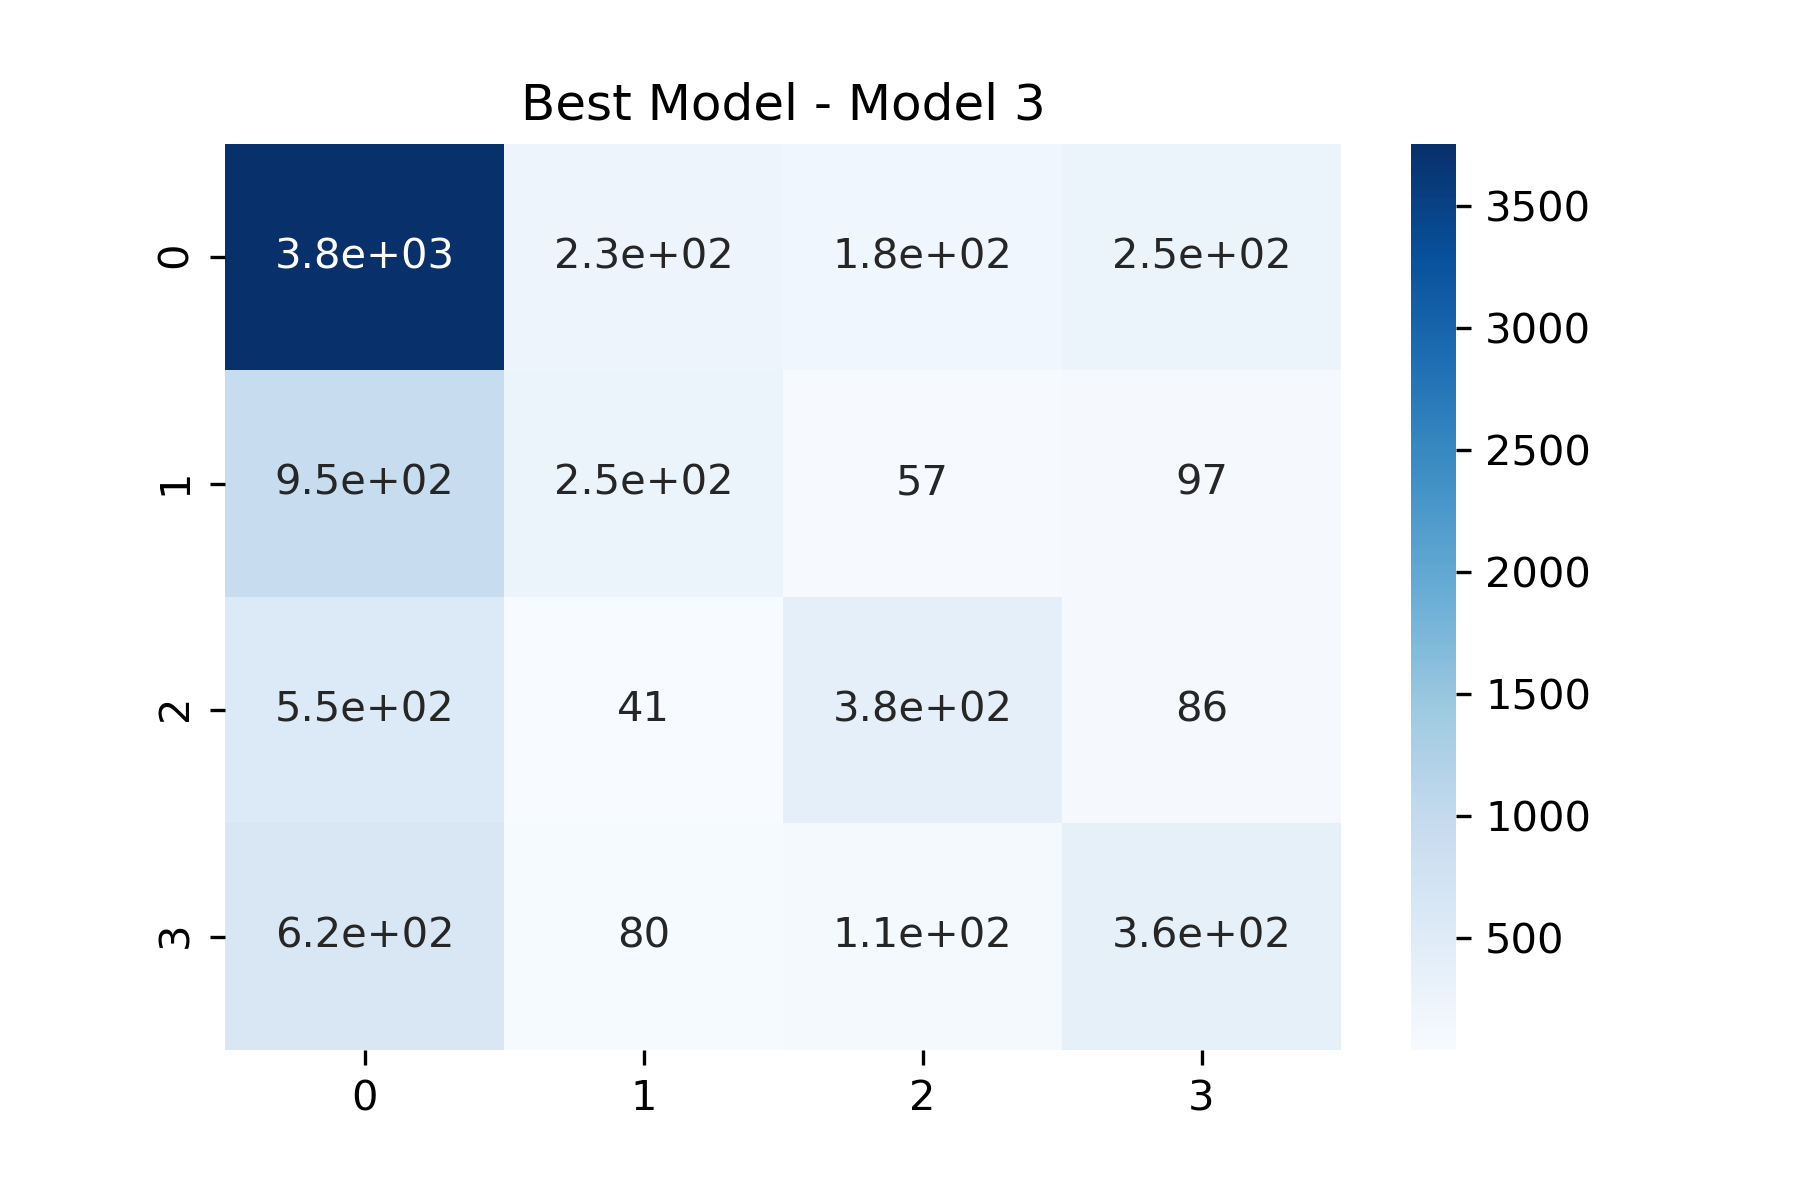
\includegraphics[scale=0.5]{figures/ns_m3cm}
    \label{fig:ns_m3cm}
}

\end{center}
\caption{Model 3 Results}
\label{fig:model3results}
\end{figure}



\begin{figure}[tbp]
\begin{center}

\subfigure[Model 4 with under-sampling - BOW]{
    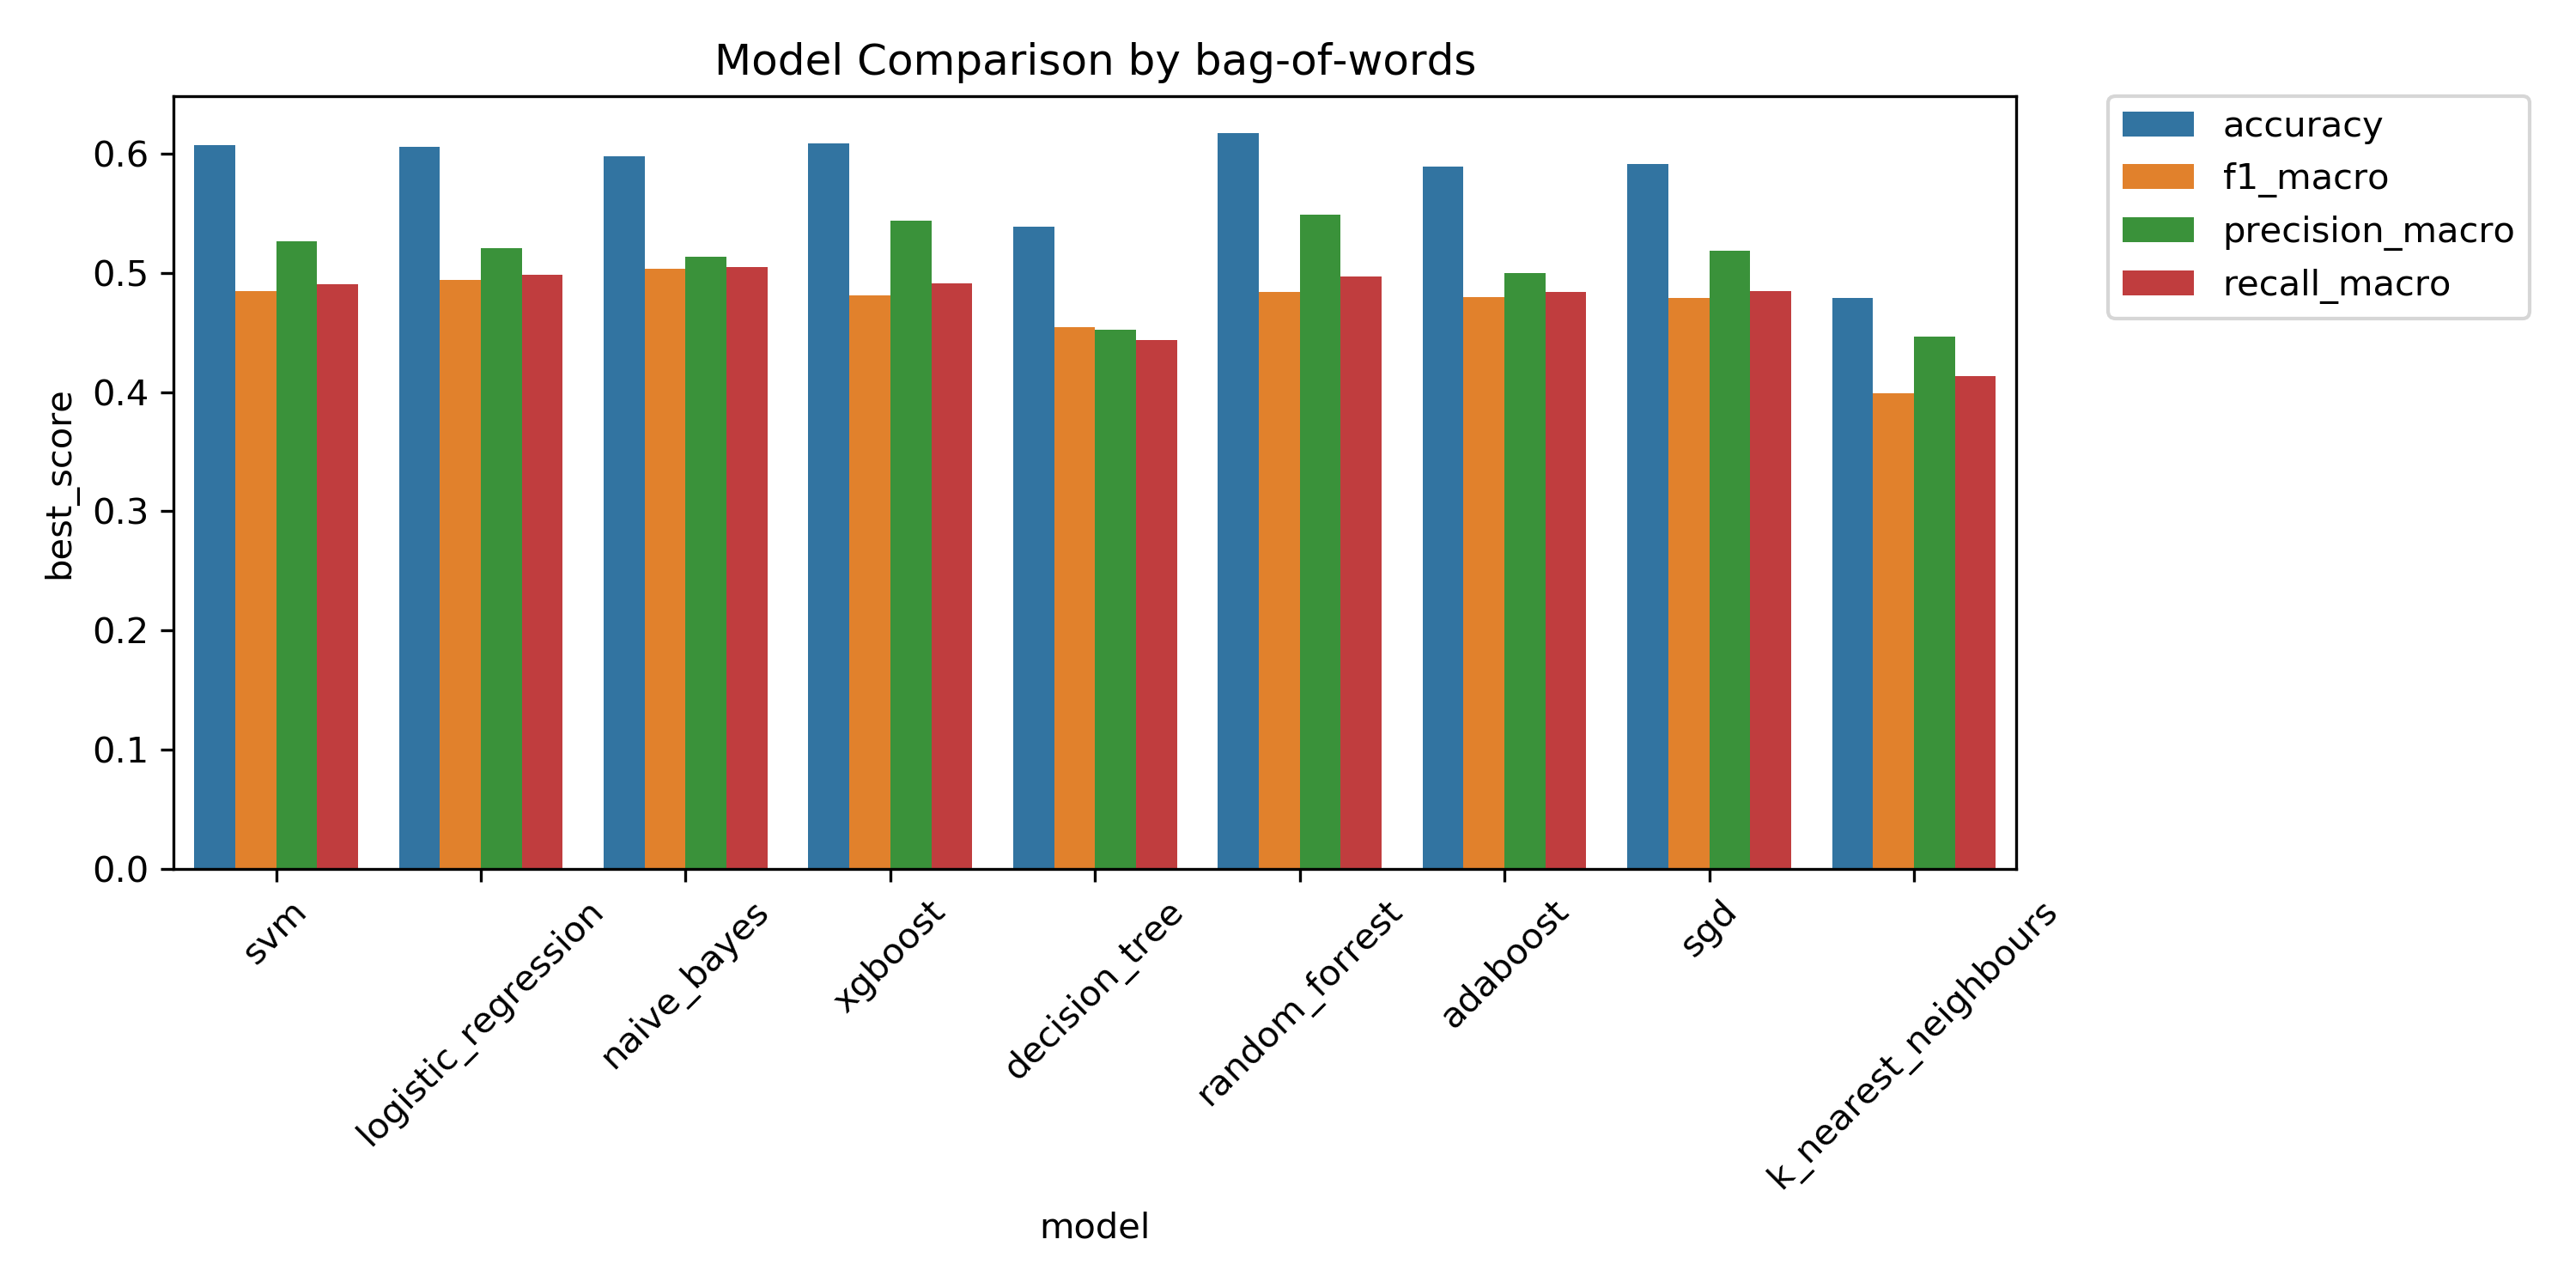
\includegraphics[scale=0.3]{figures/us_m4bow}
    \label{fig:us_m4bow}
}
\subfigure[Model 4 without under-sampling - BOW]{
    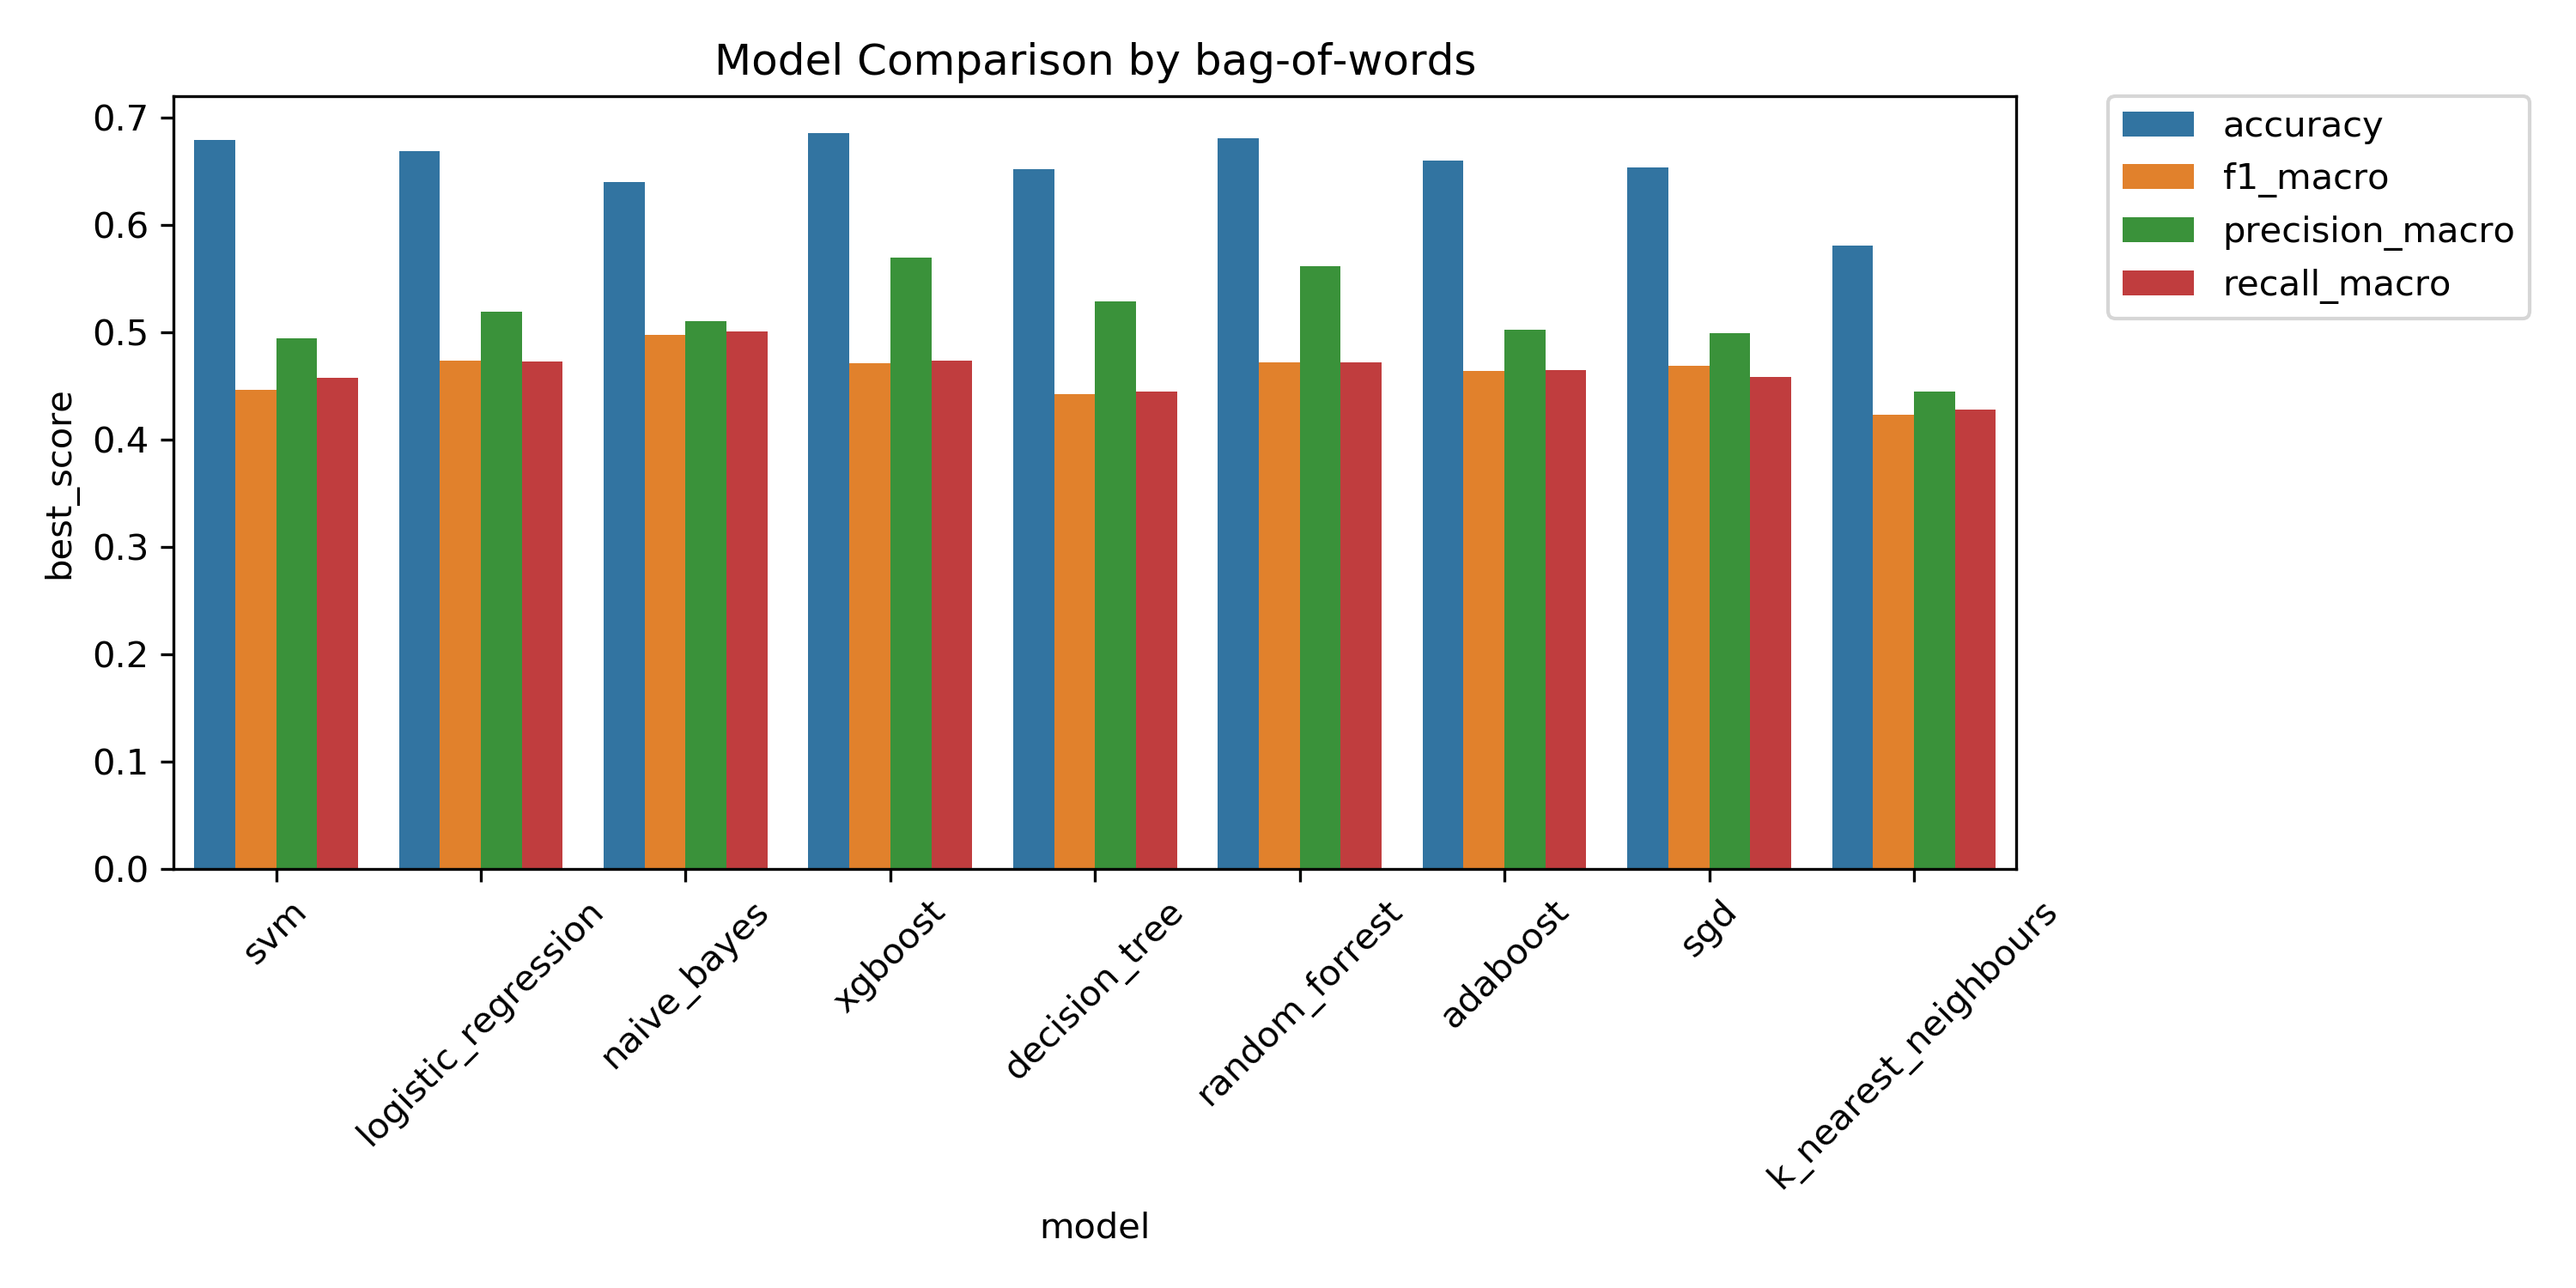
\includegraphics[scale=0.3]{figures/ns_m4bow}
    \label{fig:ns_m4bow}
}
\subfigure[Model 4 with under-sampling - TFIDF]{
    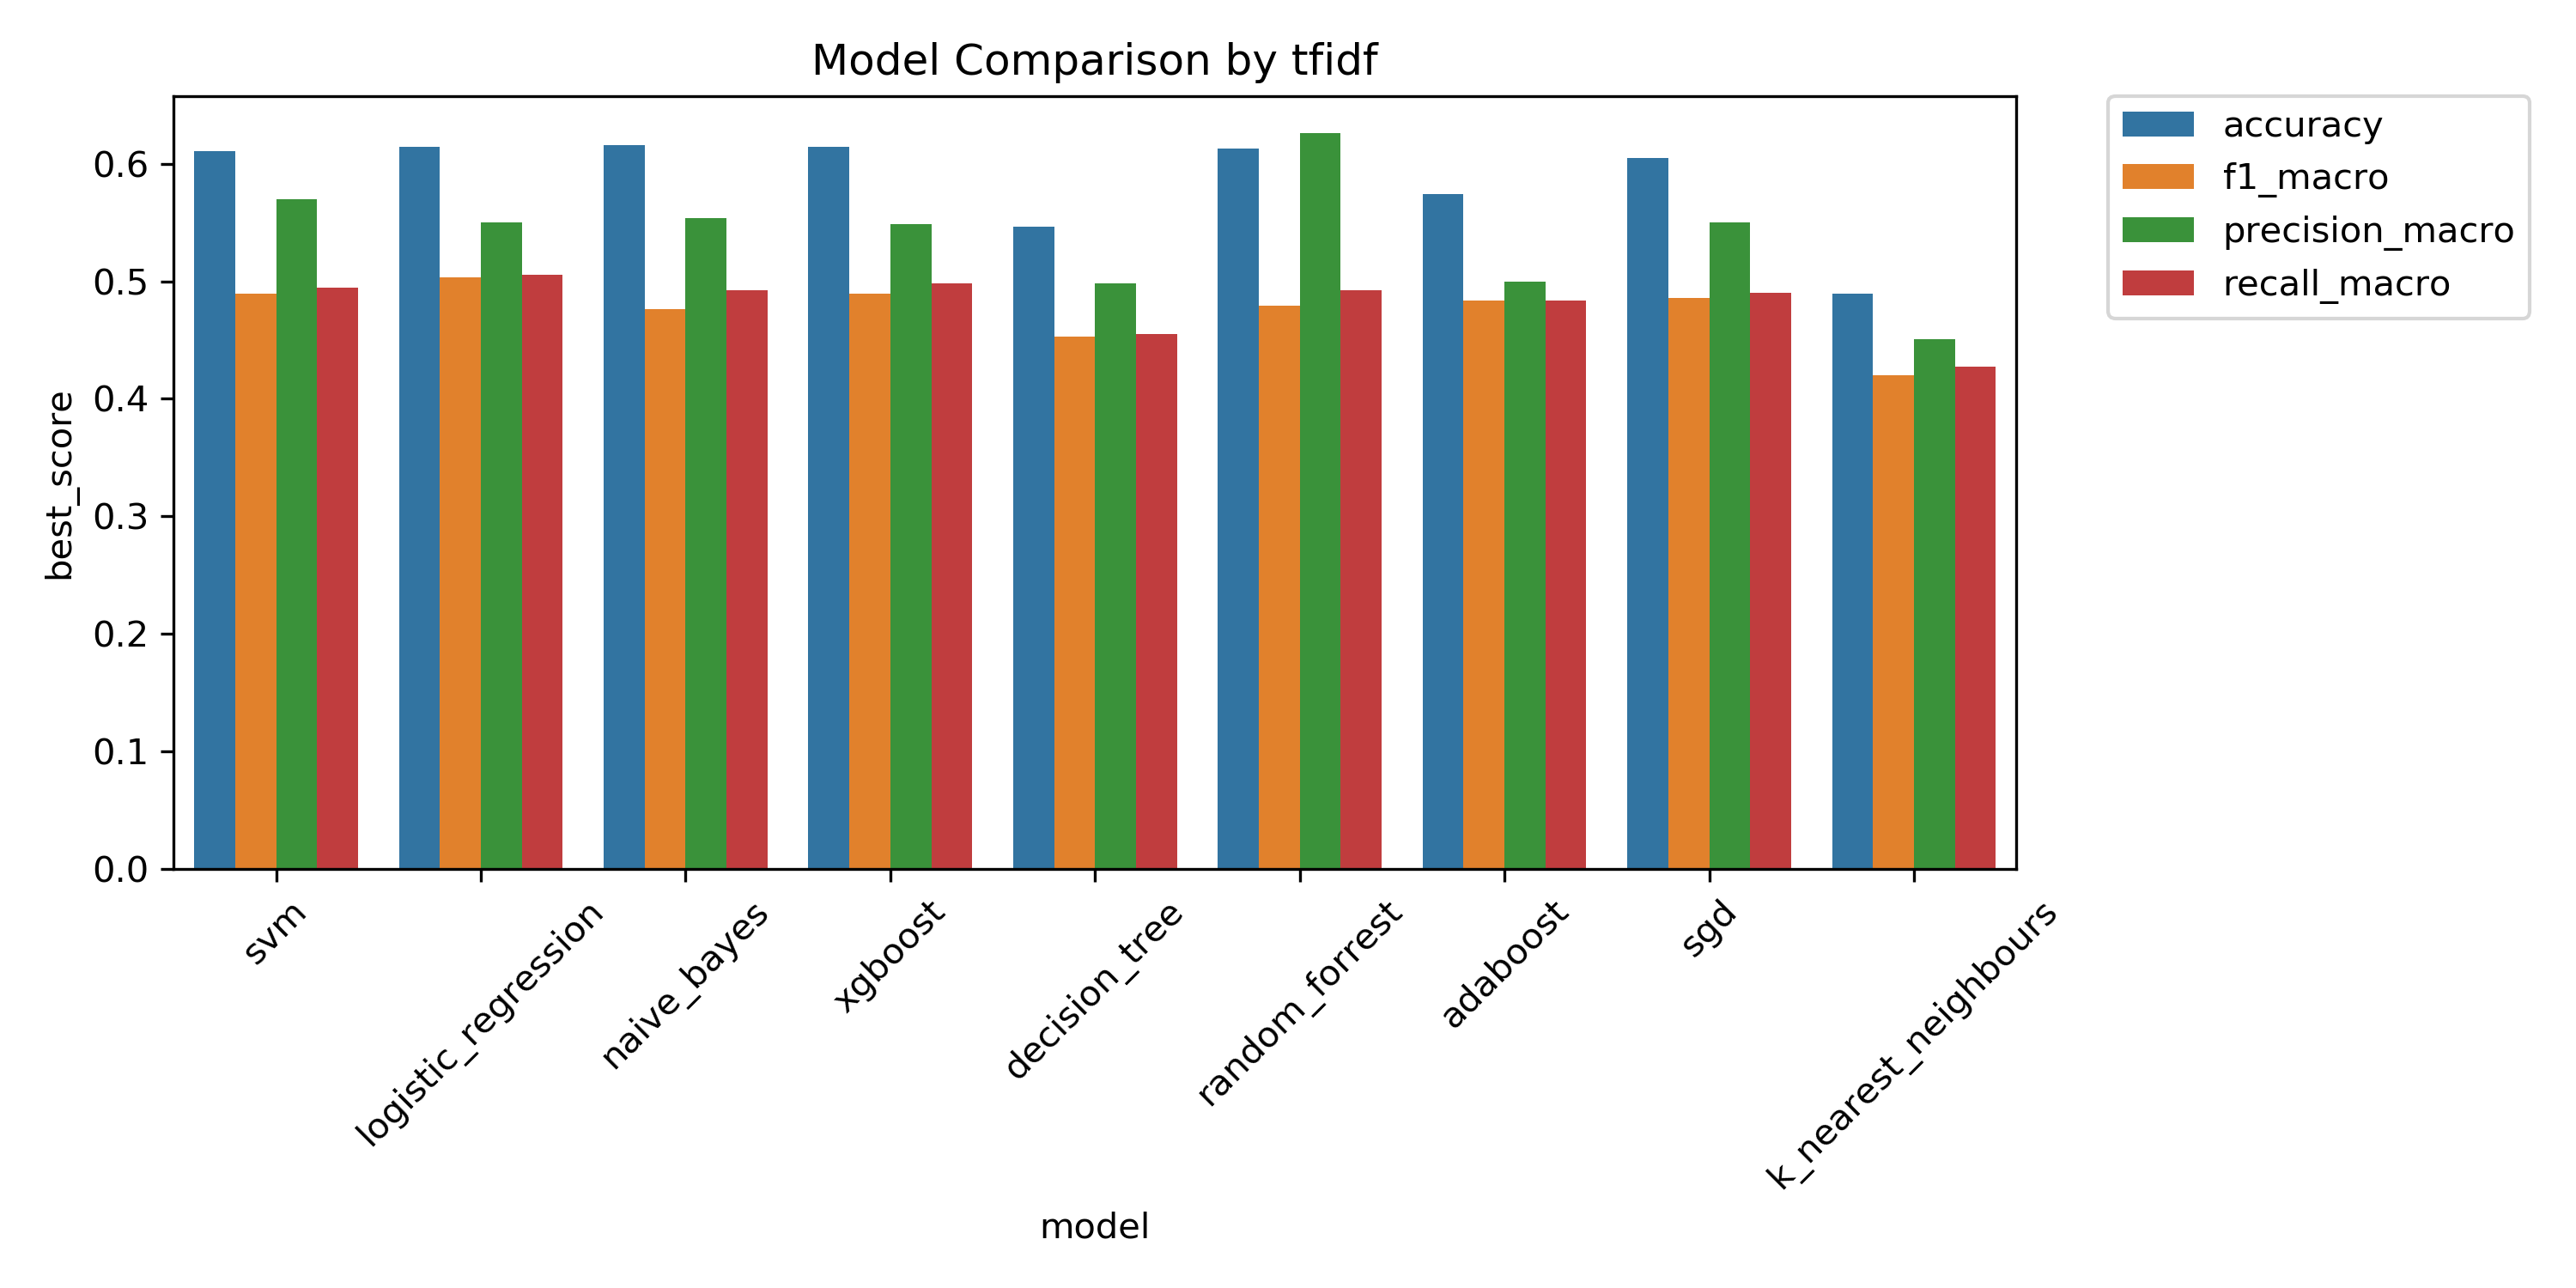
\includegraphics[scale=0.3]{figures/us_m4tfidf}
    \label{fig:us_m4tfidf}
}
\subfigure[Model 4 without under-sampling - TFIDF]{
    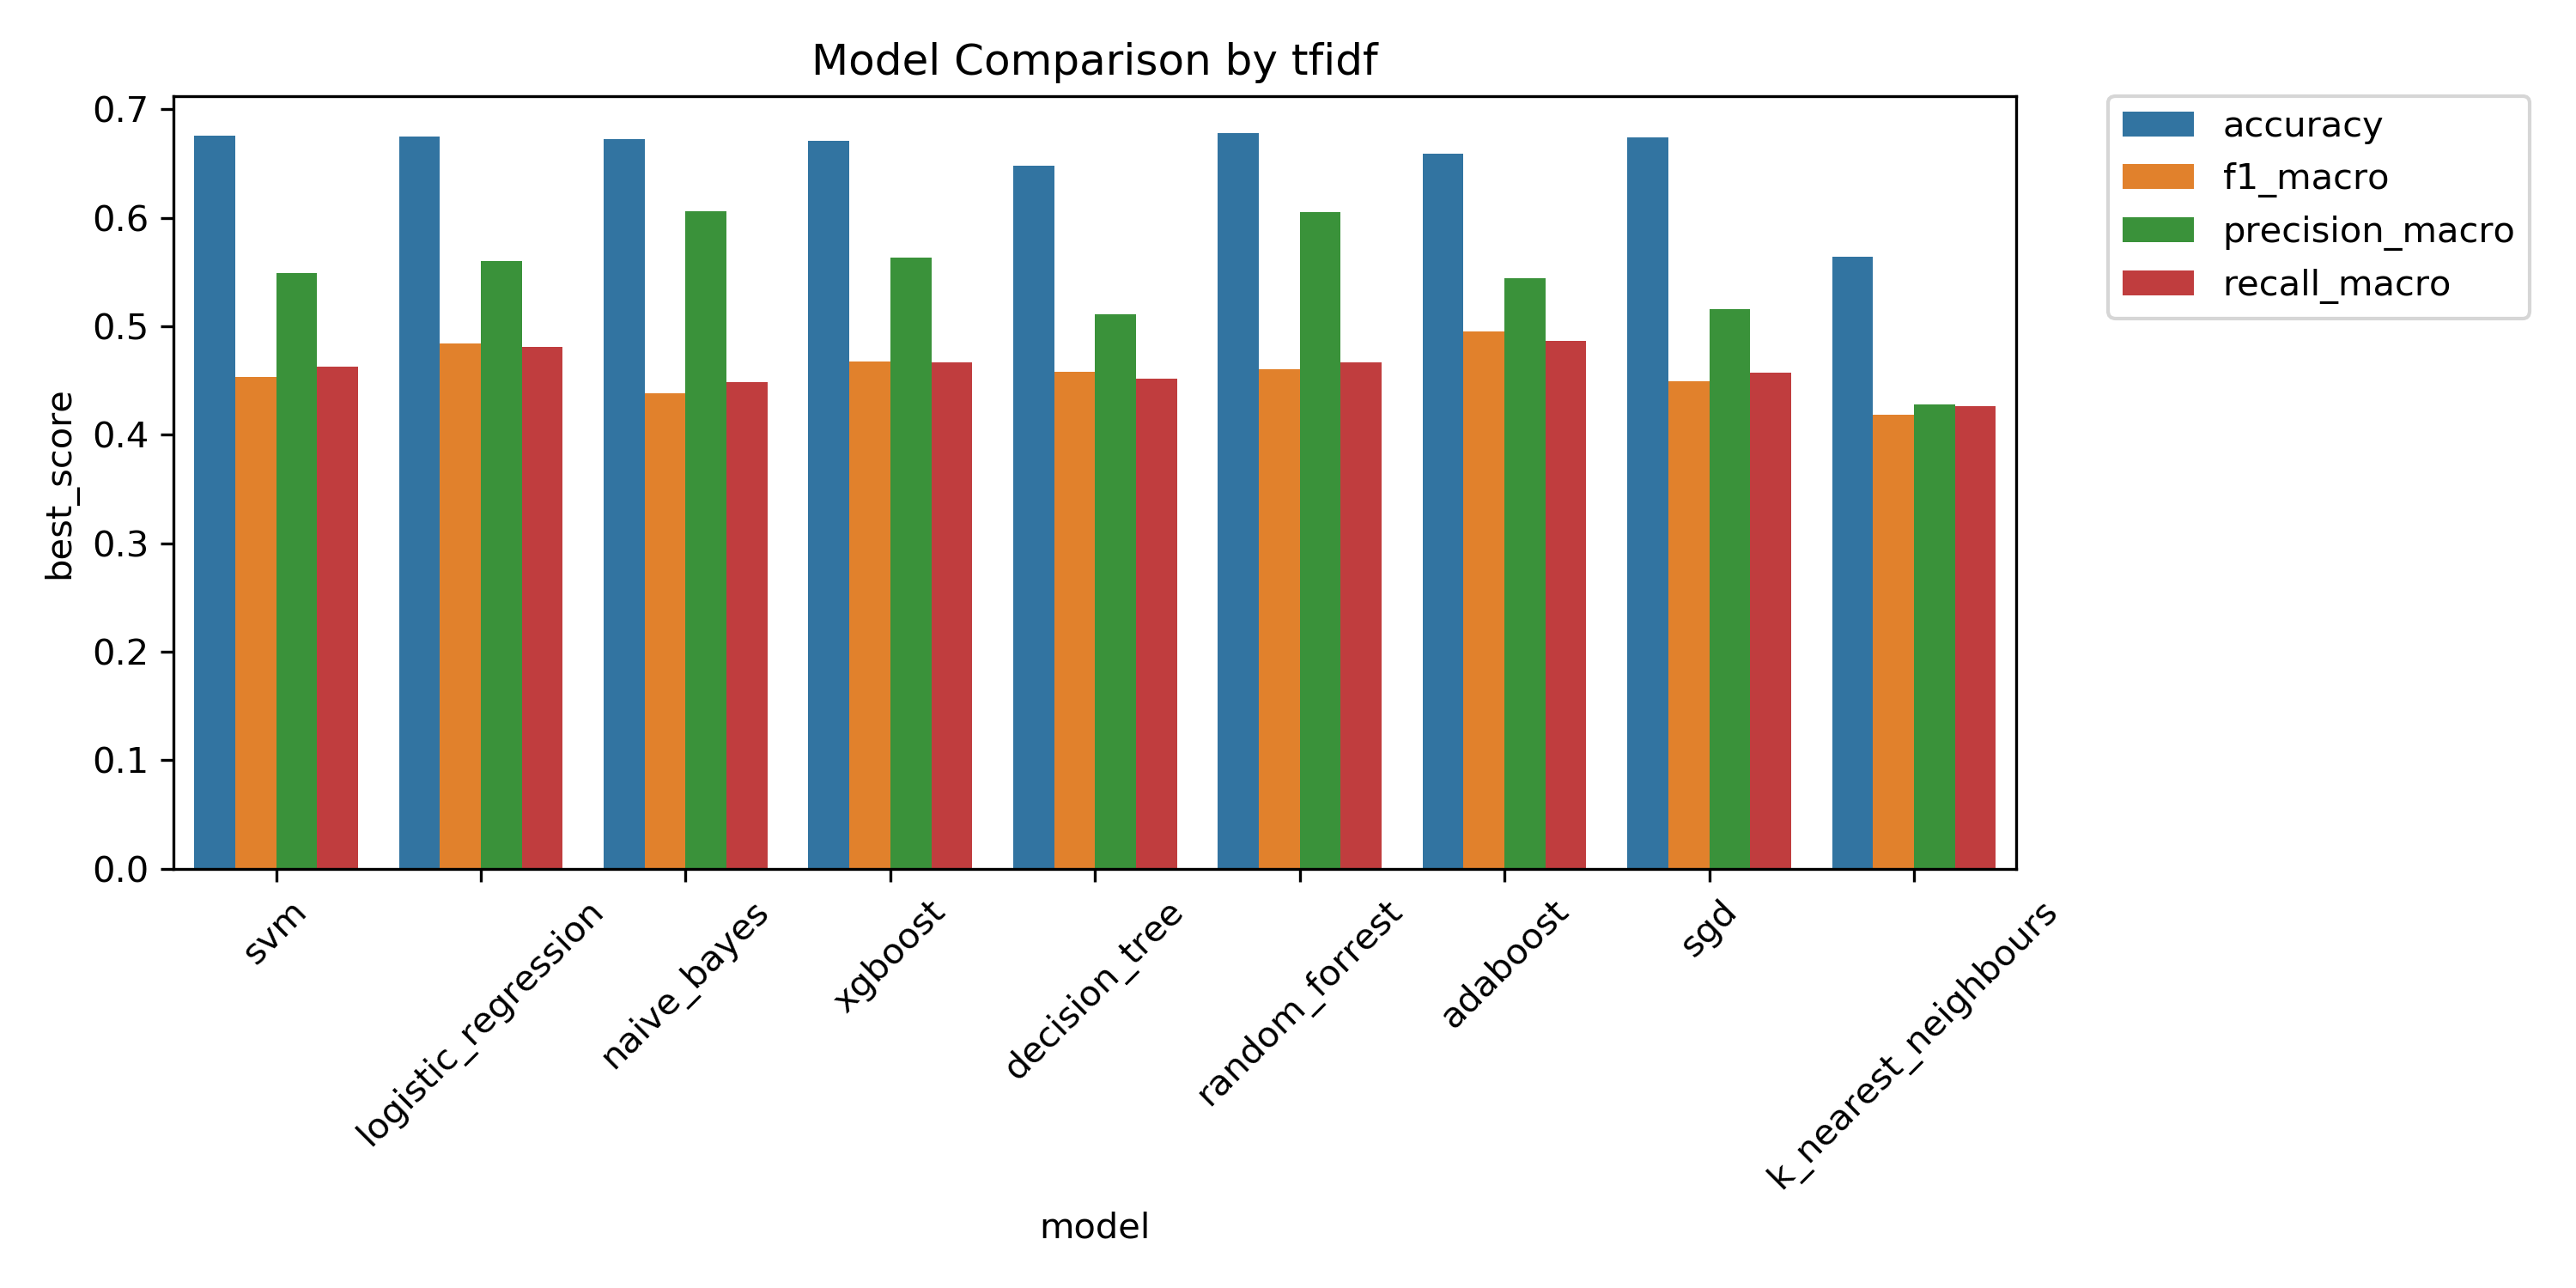
\includegraphics[scale=0.3]{figures/ns_m4tfidf}
    \label{fig:ns_m4tfidf}
}
\subfigure[Model 4 with under-sampling - CM]{
    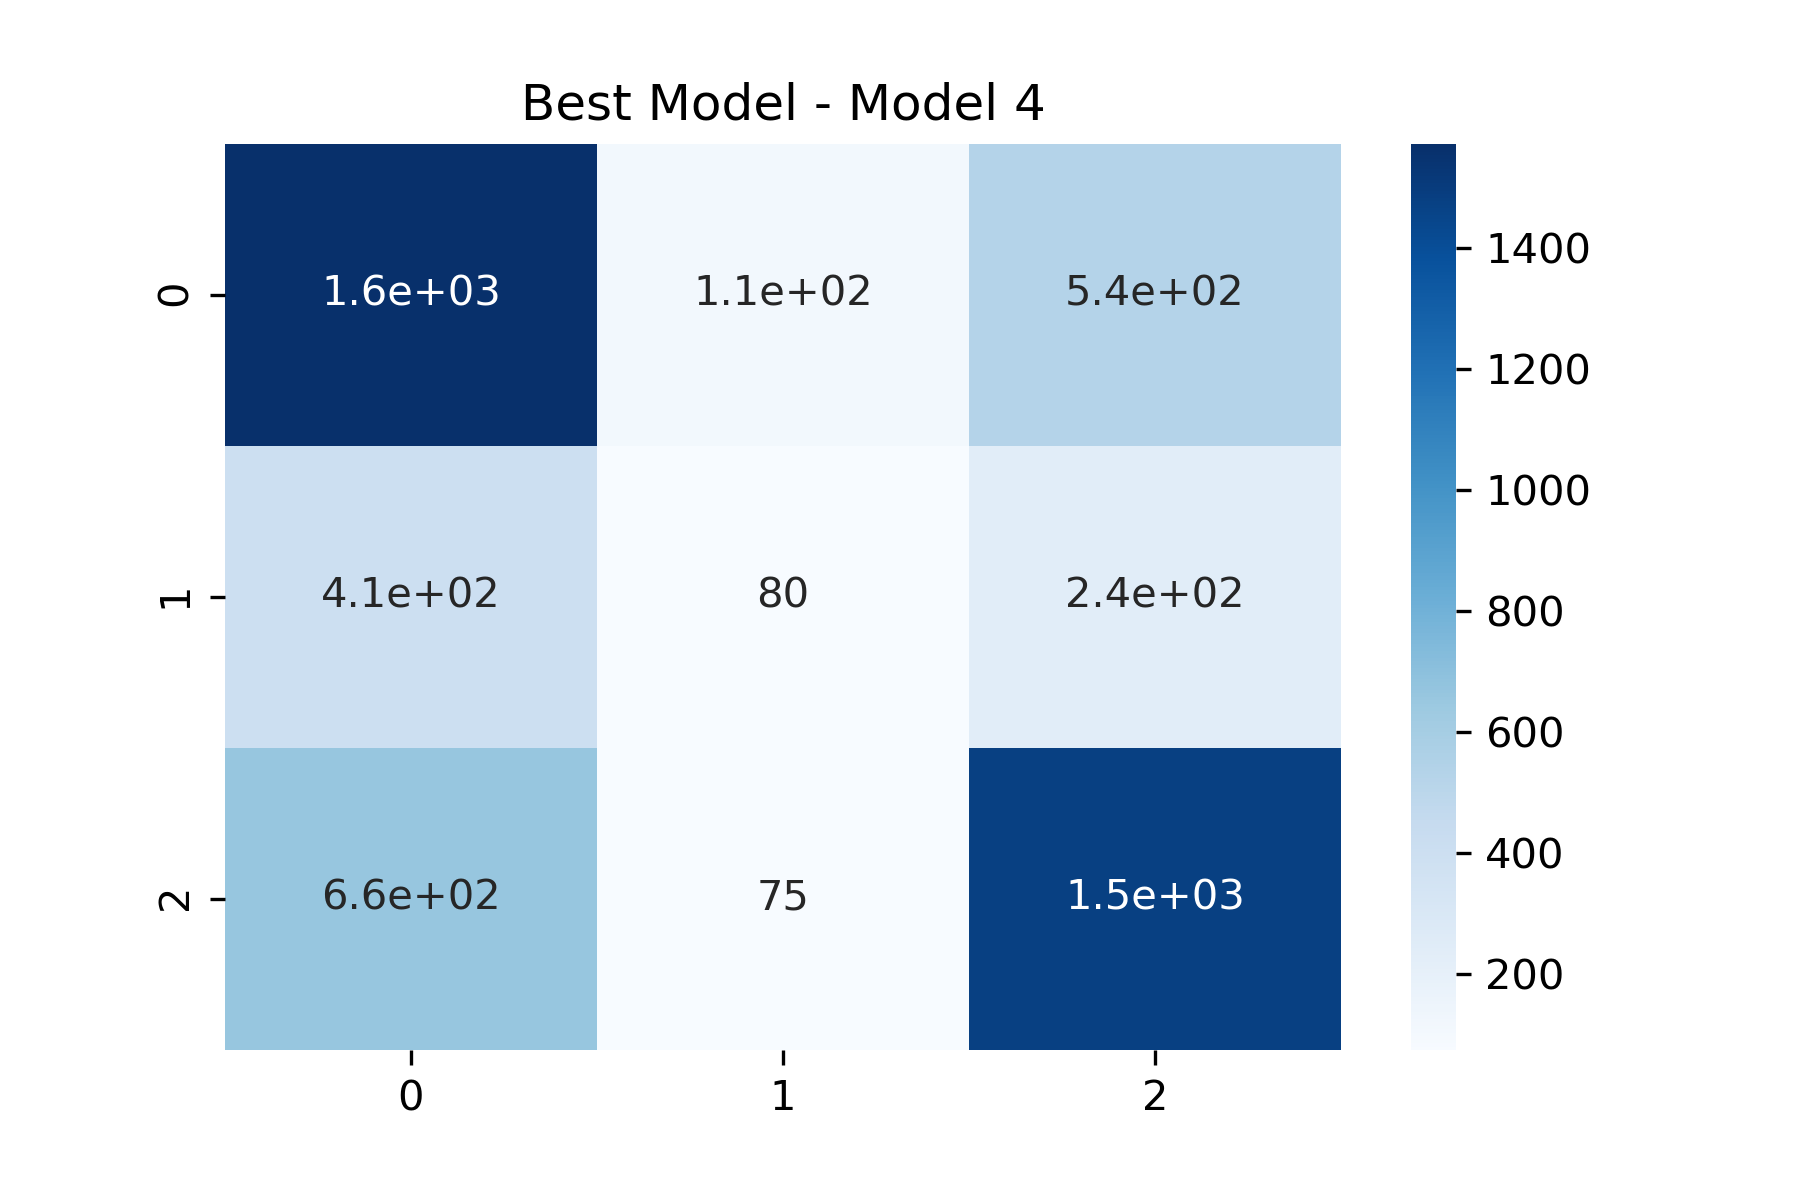
\includegraphics[scale=0.5]{figures/us_m4cm}
    \label{fig:us_m4cm}
}
\subfigure[Model 4 without under-sampling - CM]{
    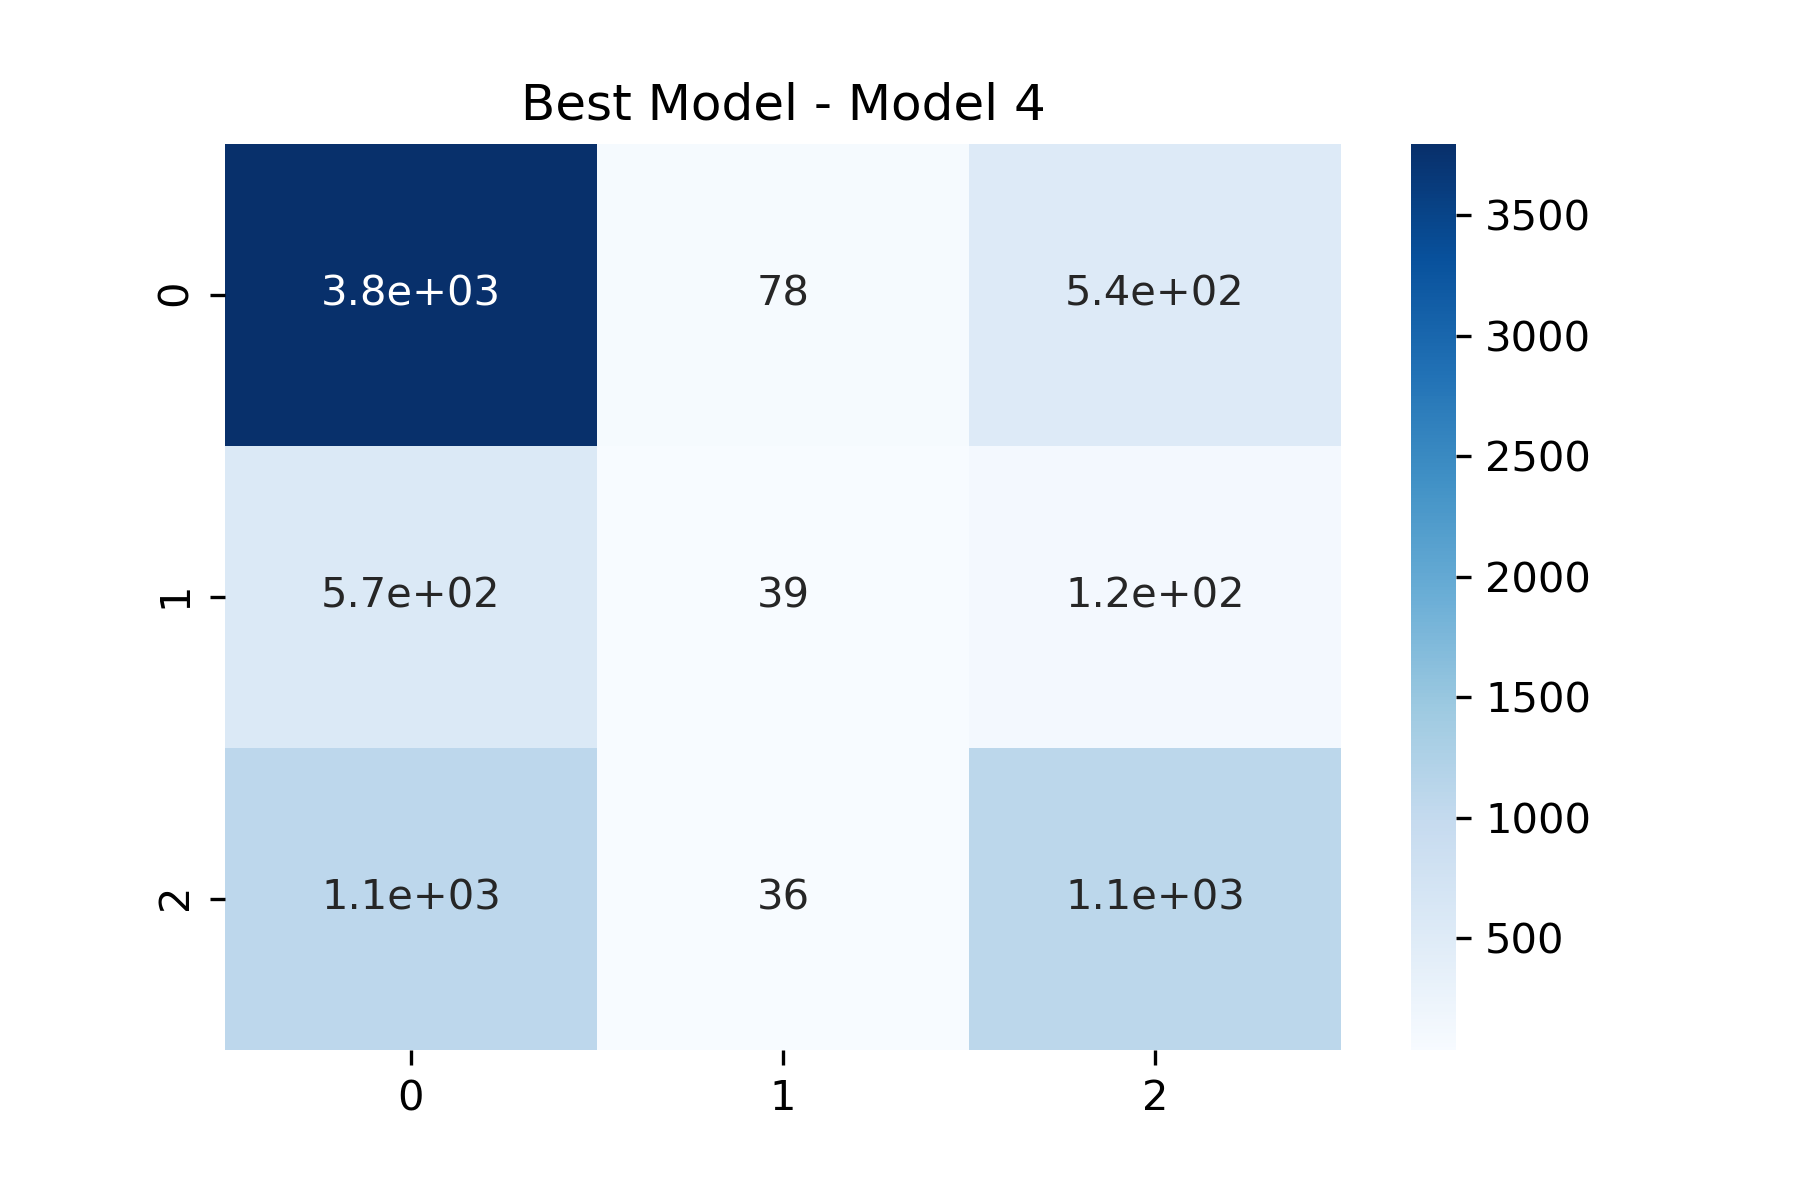
\includegraphics[scale=0.5]{figures/ns_m4cm}
    \label{fig:ns_m4cm}
}

\end{center}
\caption{Model 4 Results}
\label{fig:model4results}
\end{figure}






\begin{figure}[tbp]
\begin{center}

\subfigure[Model 5 with under-sampling - BOW]{
    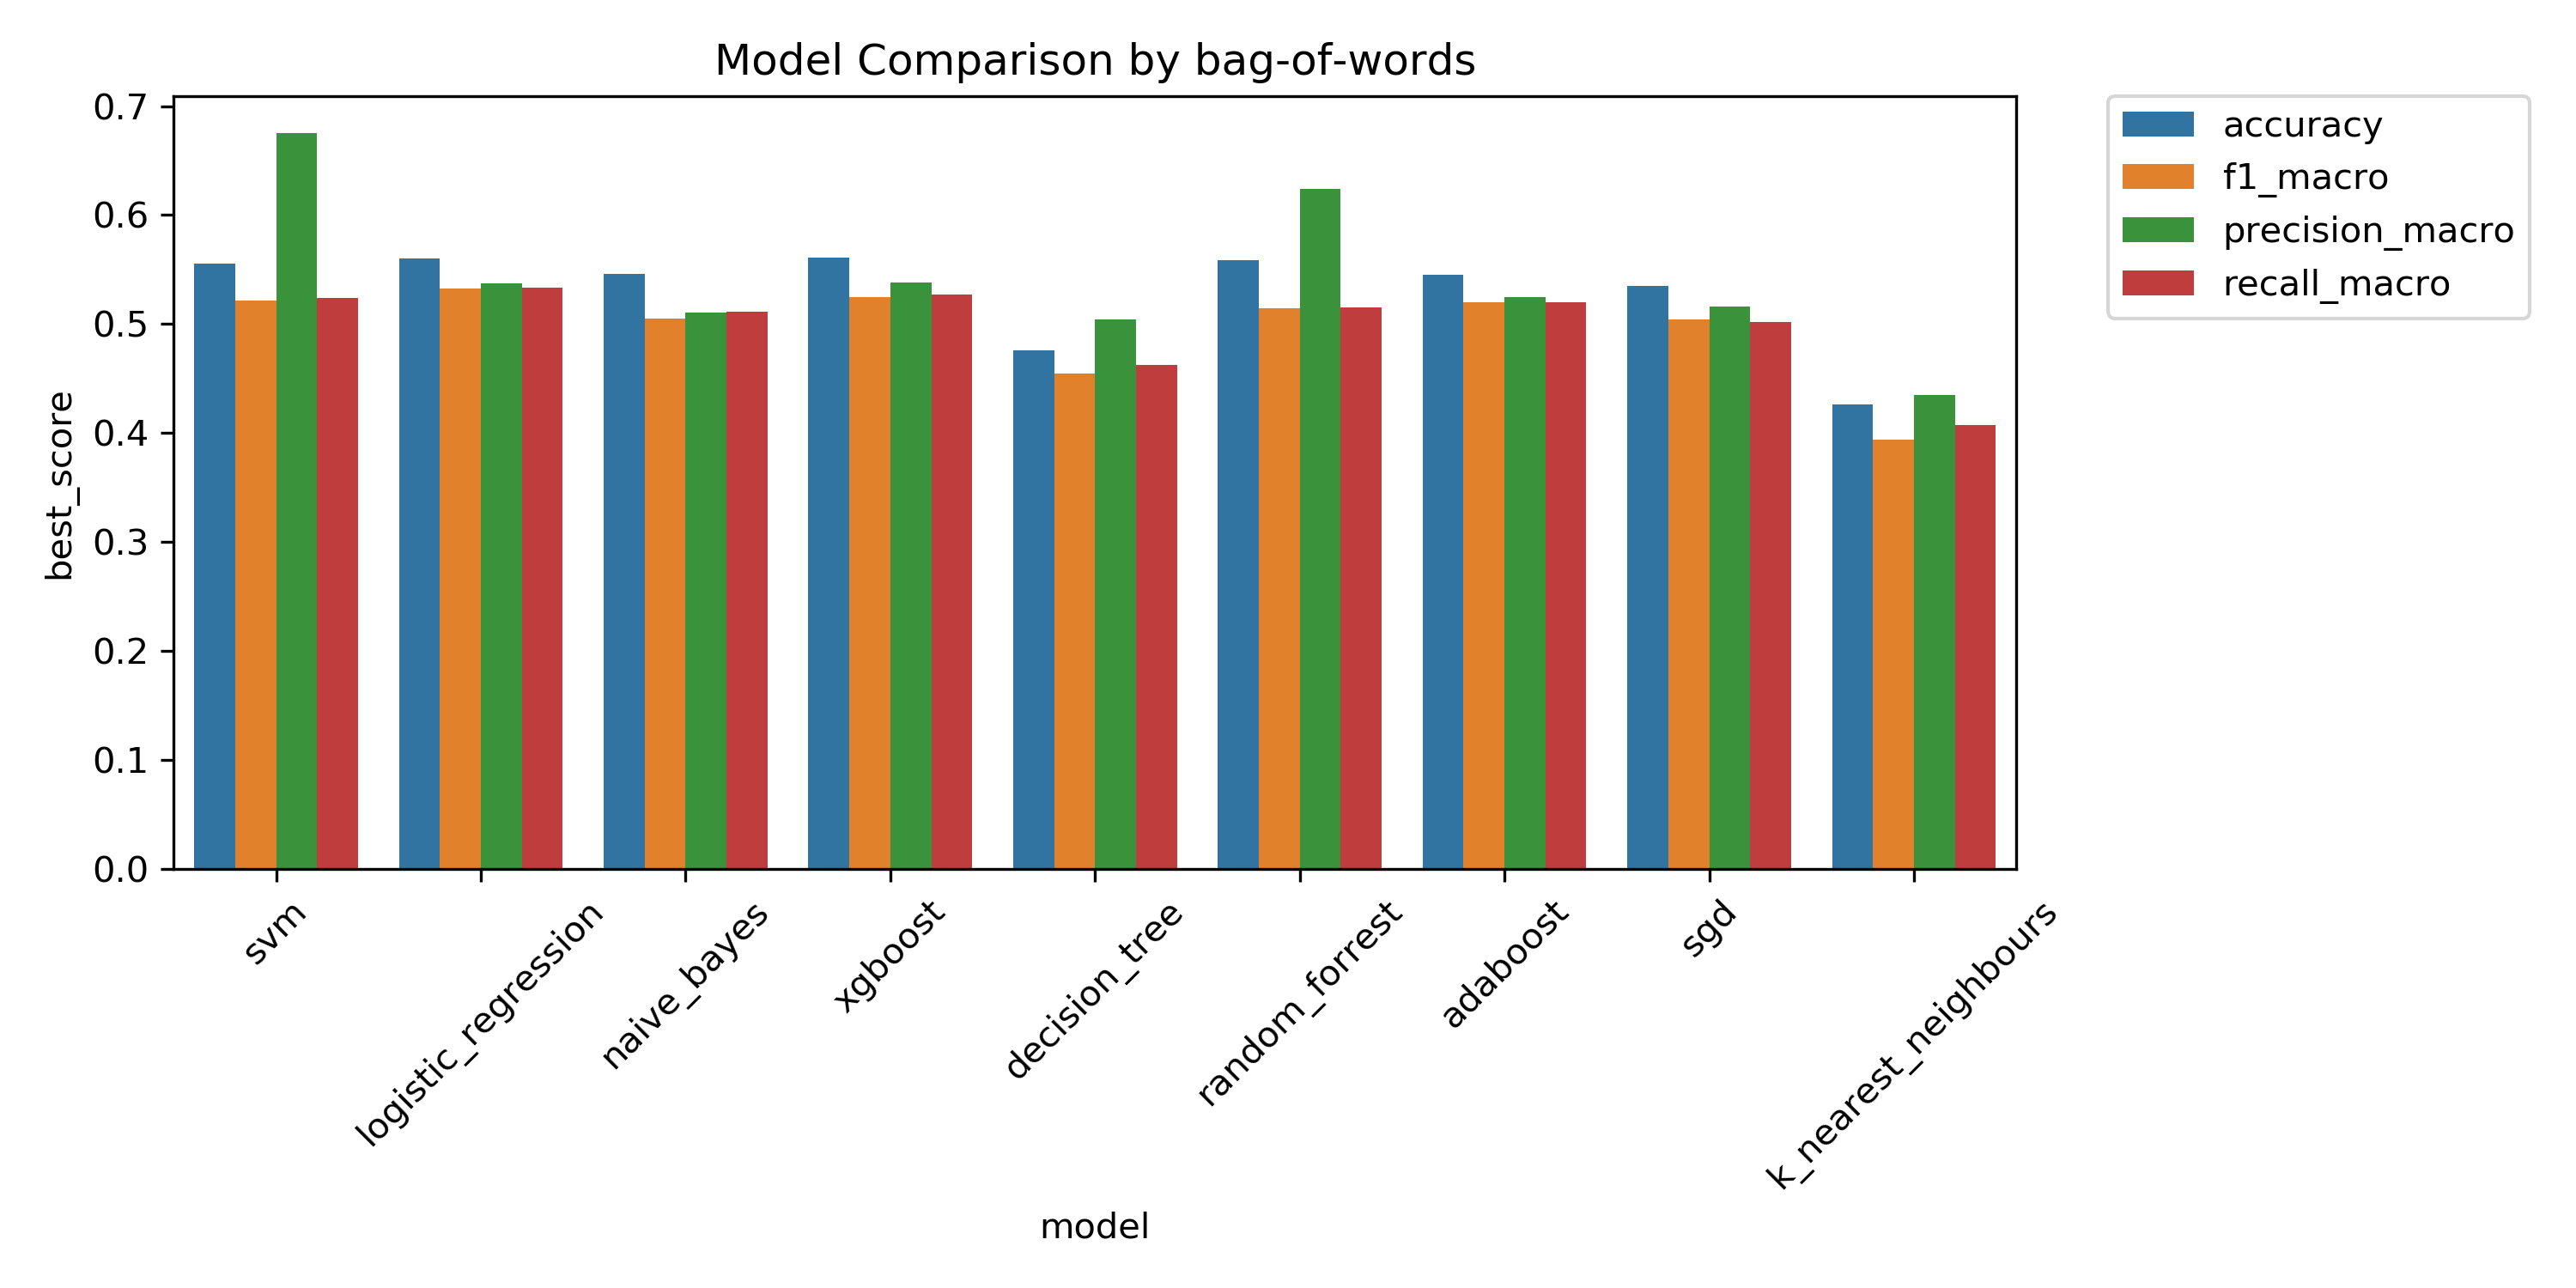
\includegraphics[scale=0.3]{figures/us_m5bow}
    \label{fig:us_m5bow}
}
\subfigure[Model 5 without under-sampling - BOW]{
    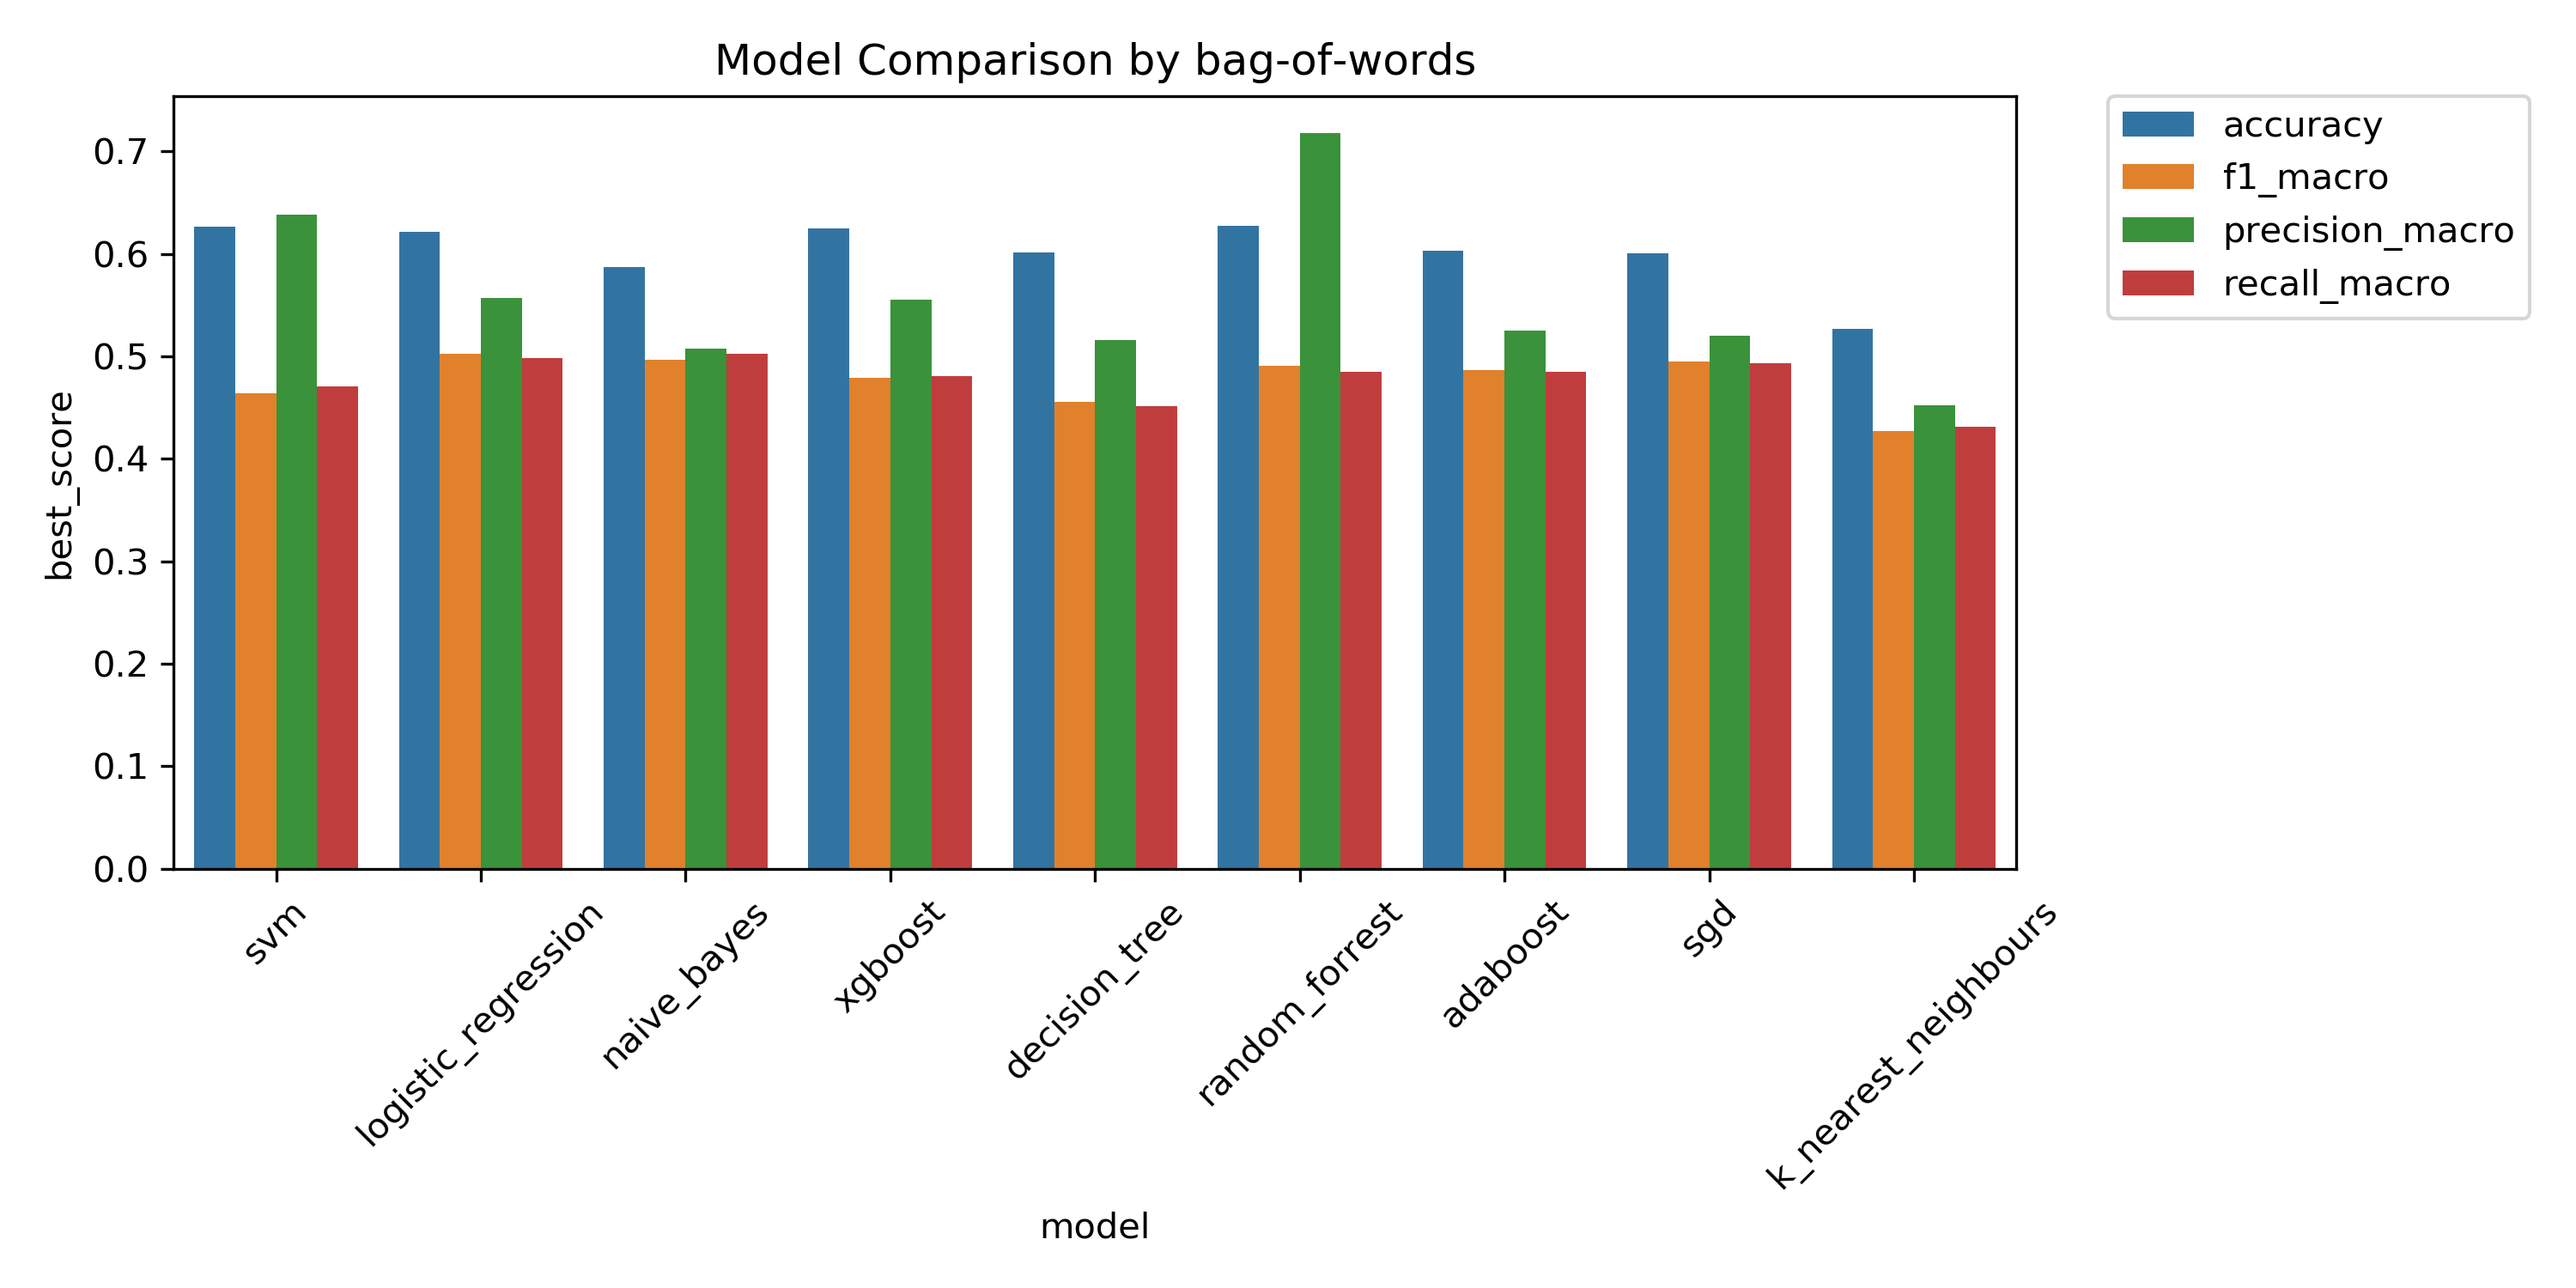
\includegraphics[scale=0.3]{figures/ns_m5bow}
    \label{fig:ns_m5bow}
}
\subfigure[Model 5 with under-sampling - TFIDF]{
    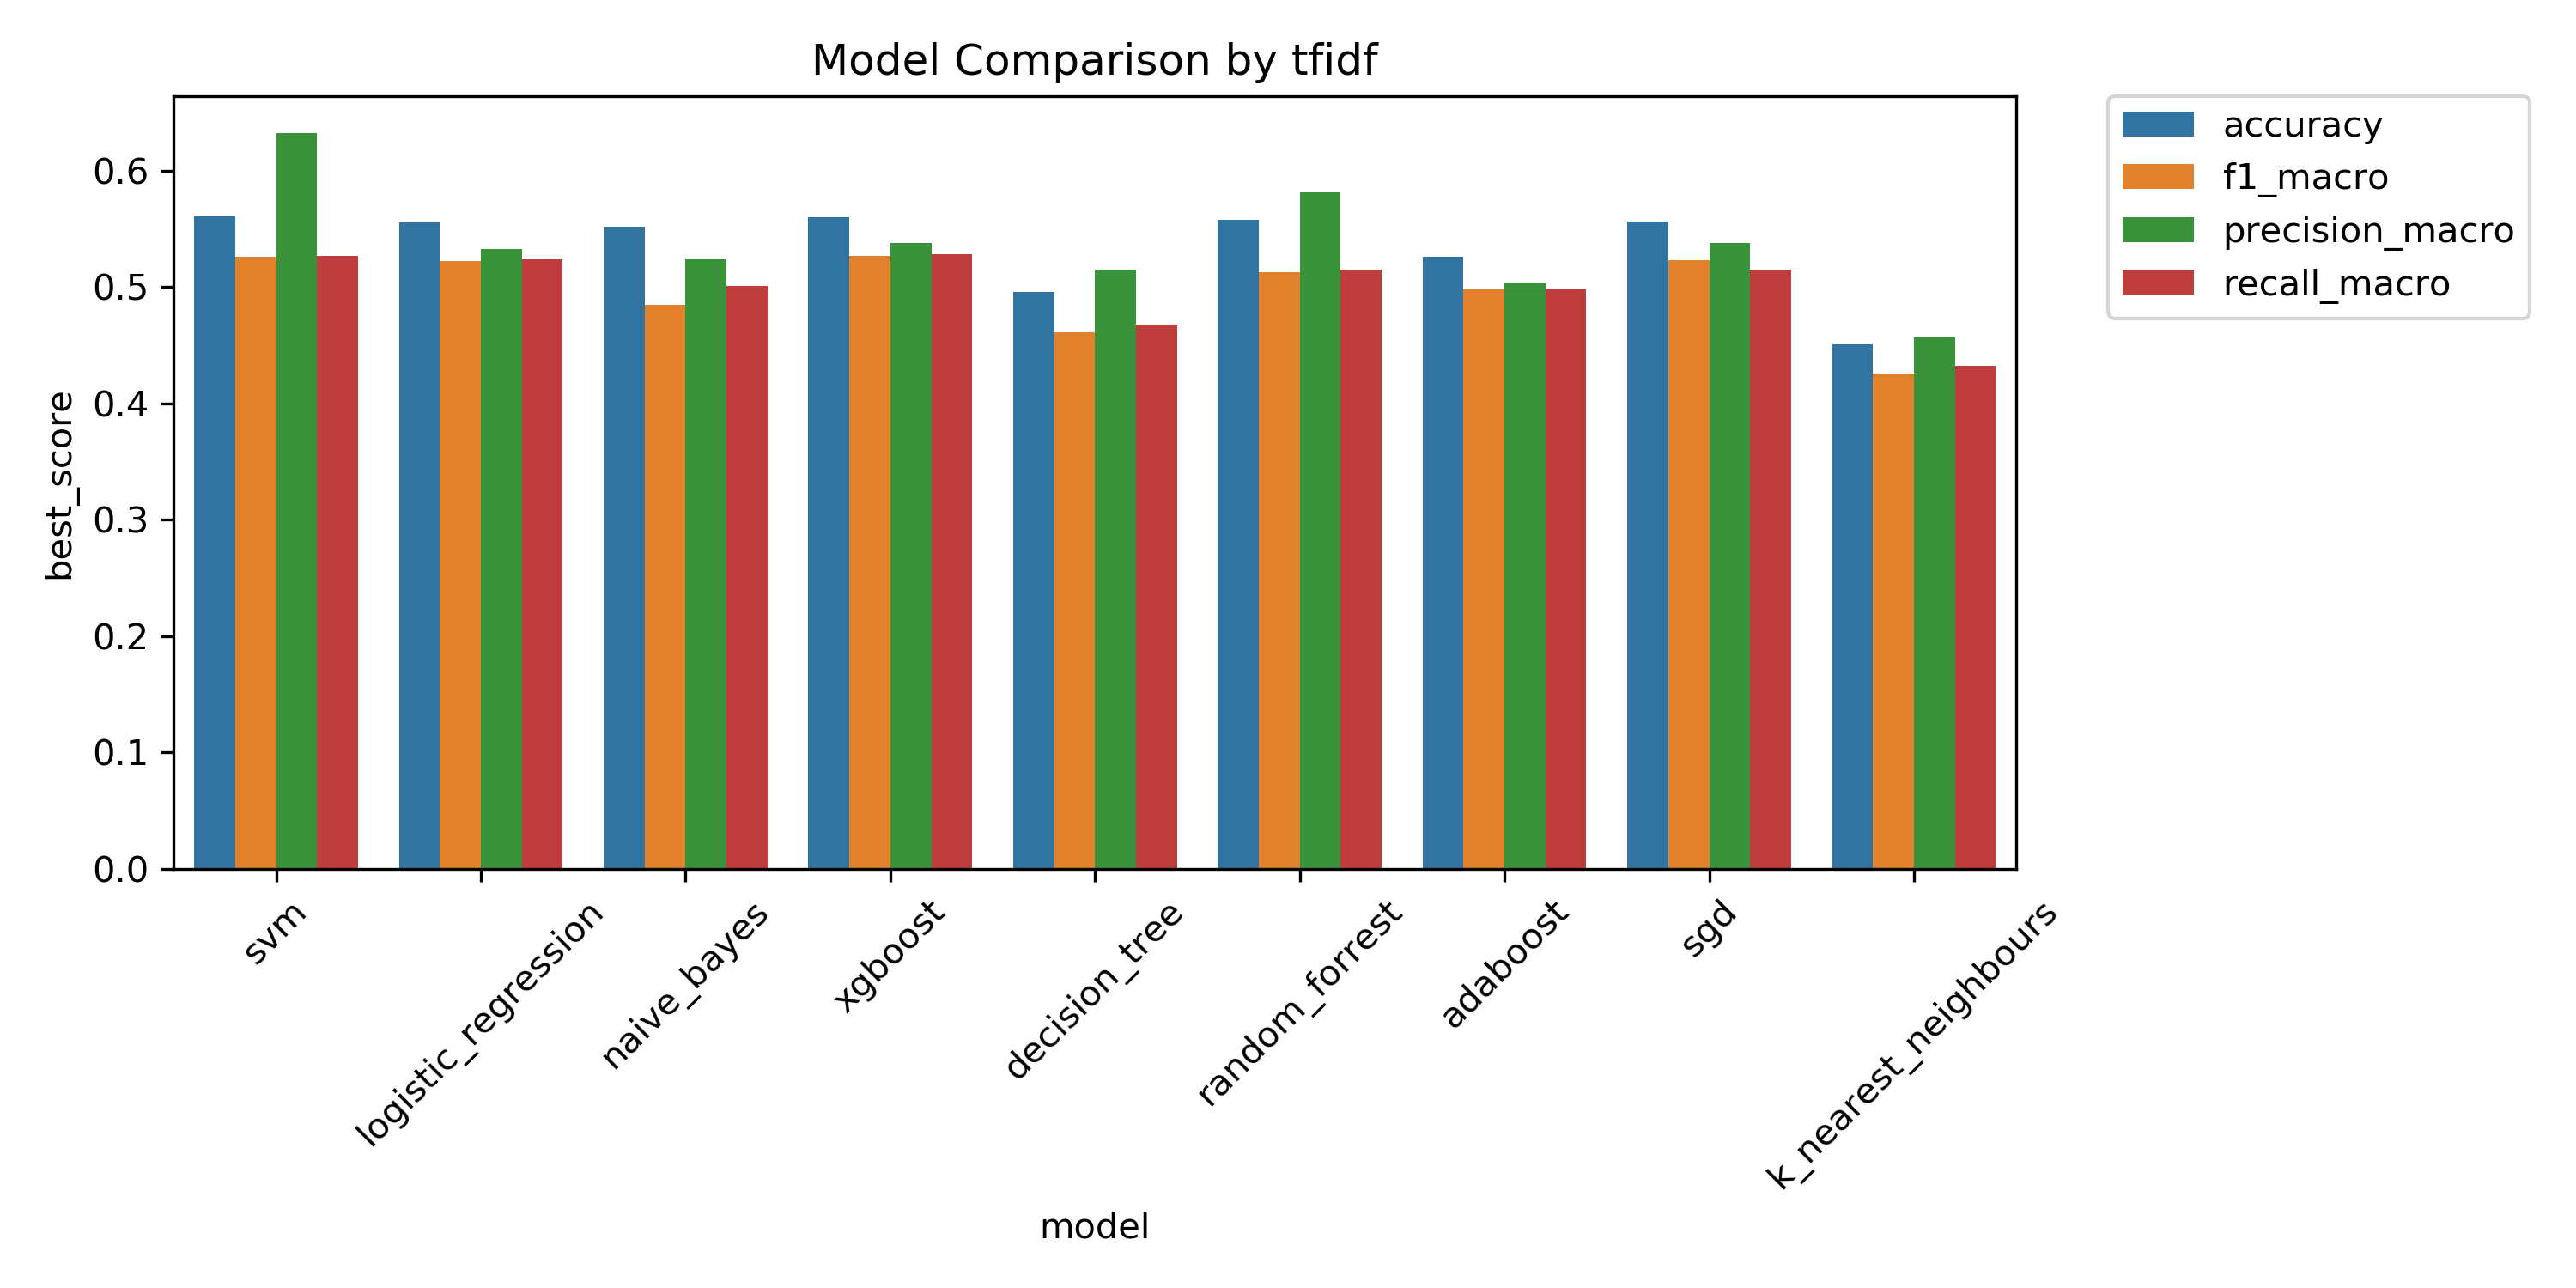
\includegraphics[scale=0.3]{figures/us_m5tfidf}
    \label{fig:us_m5tfidf}
}
\subfigure[Model 5 without under-sampling - TFIDF]{
    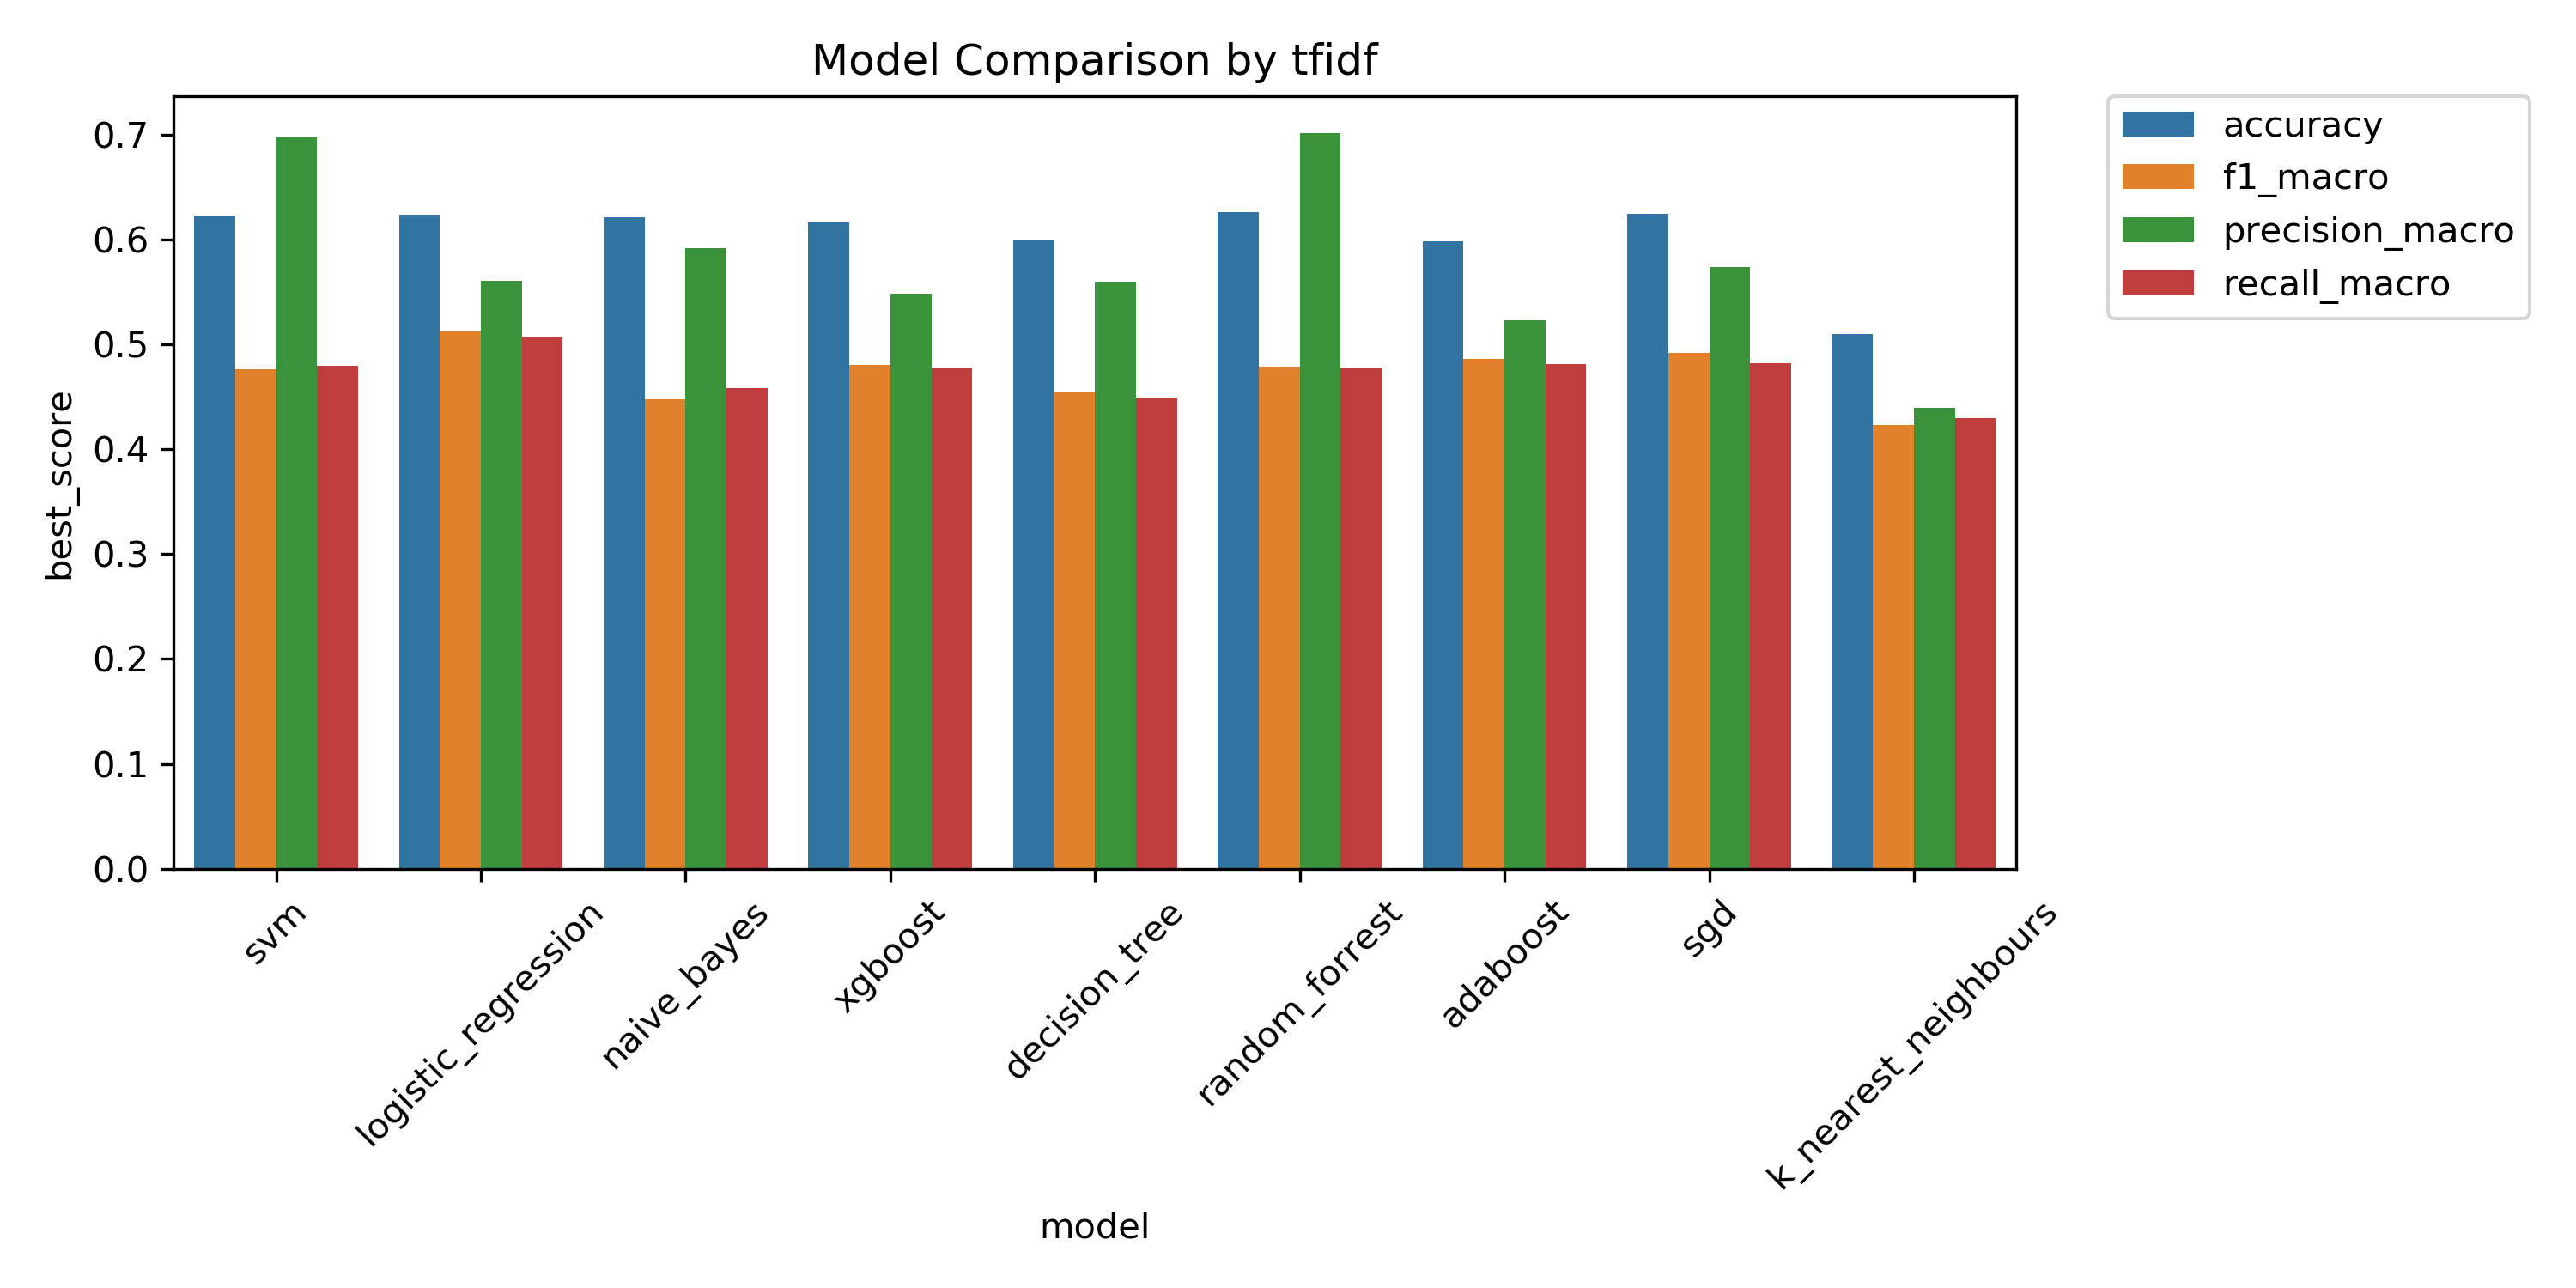
\includegraphics[scale=0.3]{figures/ns_m5tfidf}
    \label{fig:ns_m5tfidf}
}
\subfigure[Model 5 with under-sampling - CM]{
    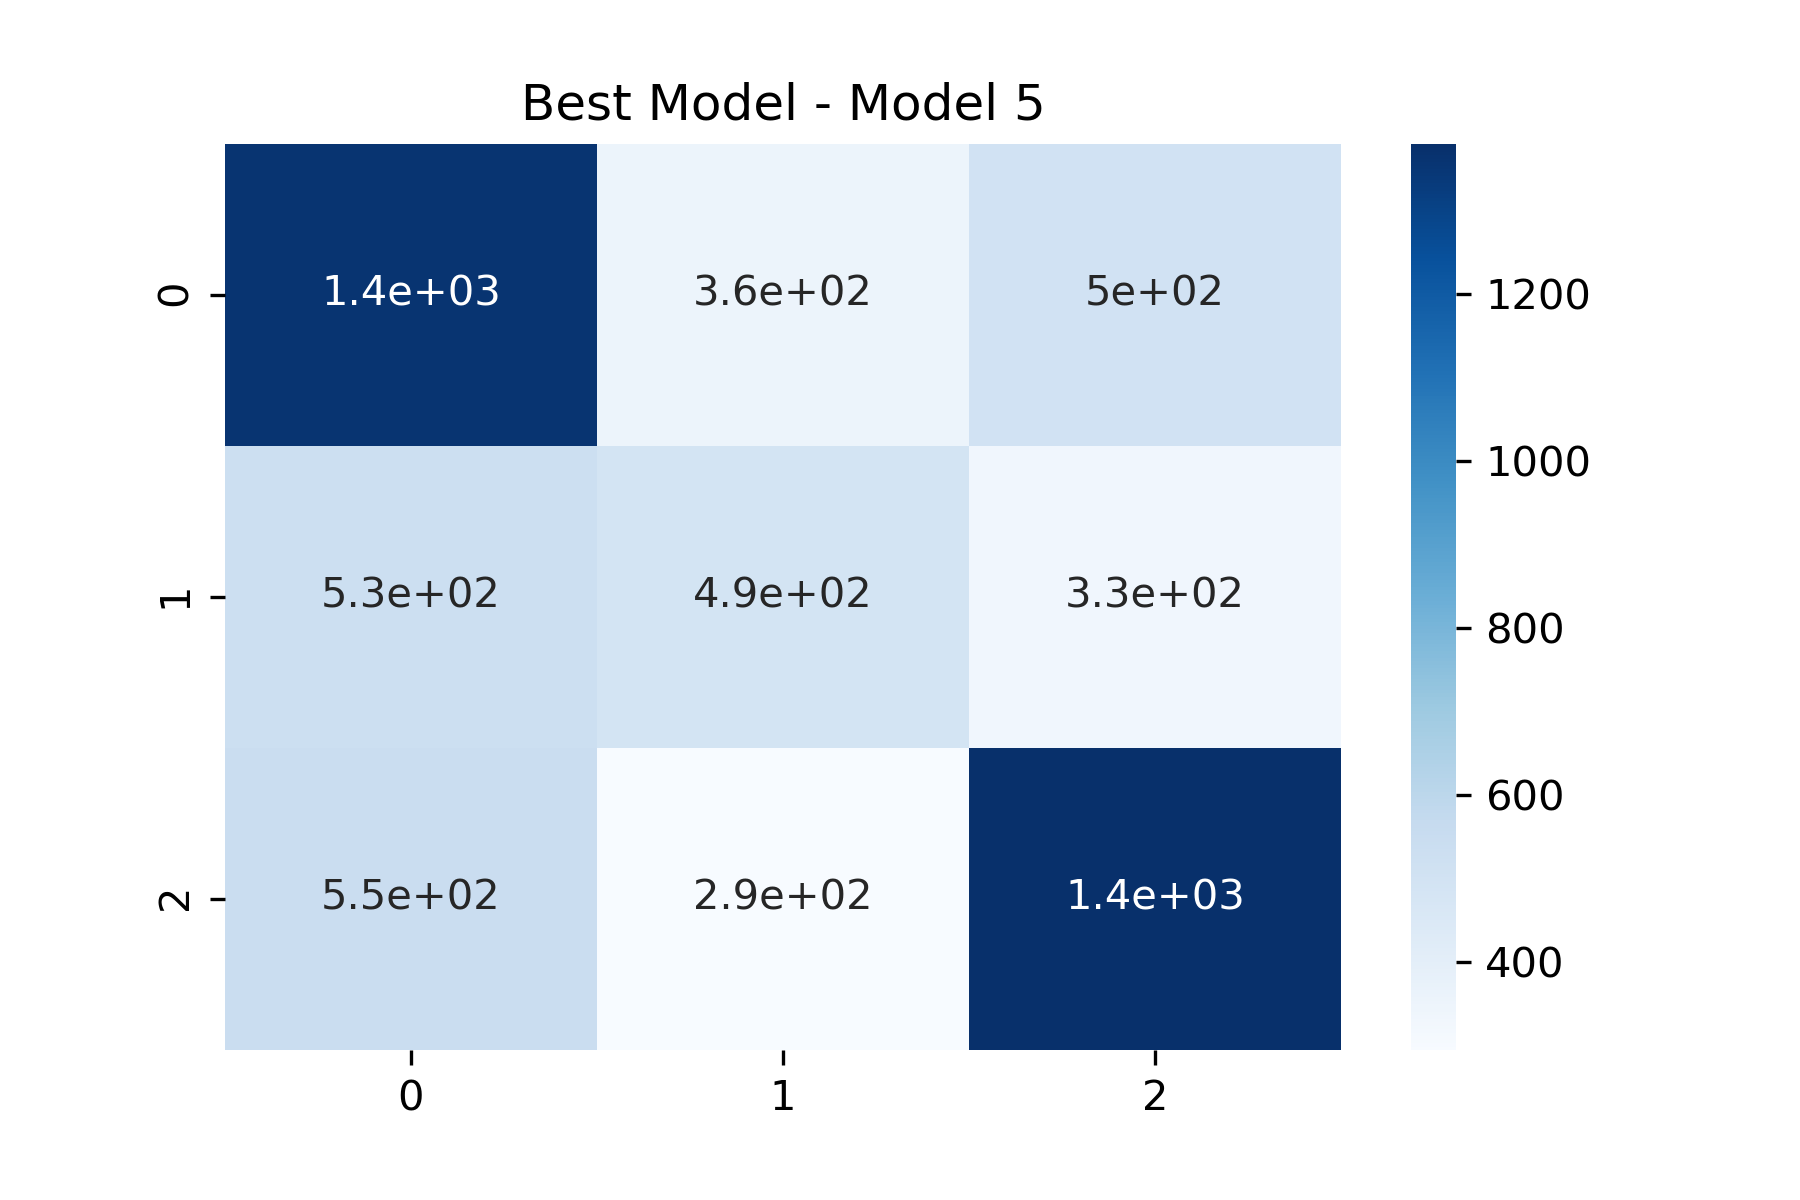
\includegraphics[scale=0.5]{figures/us_m5cm}
    \label{fig:us_m5cm}
}
\subfigure[Model 5 without under-sampling - CM]{
    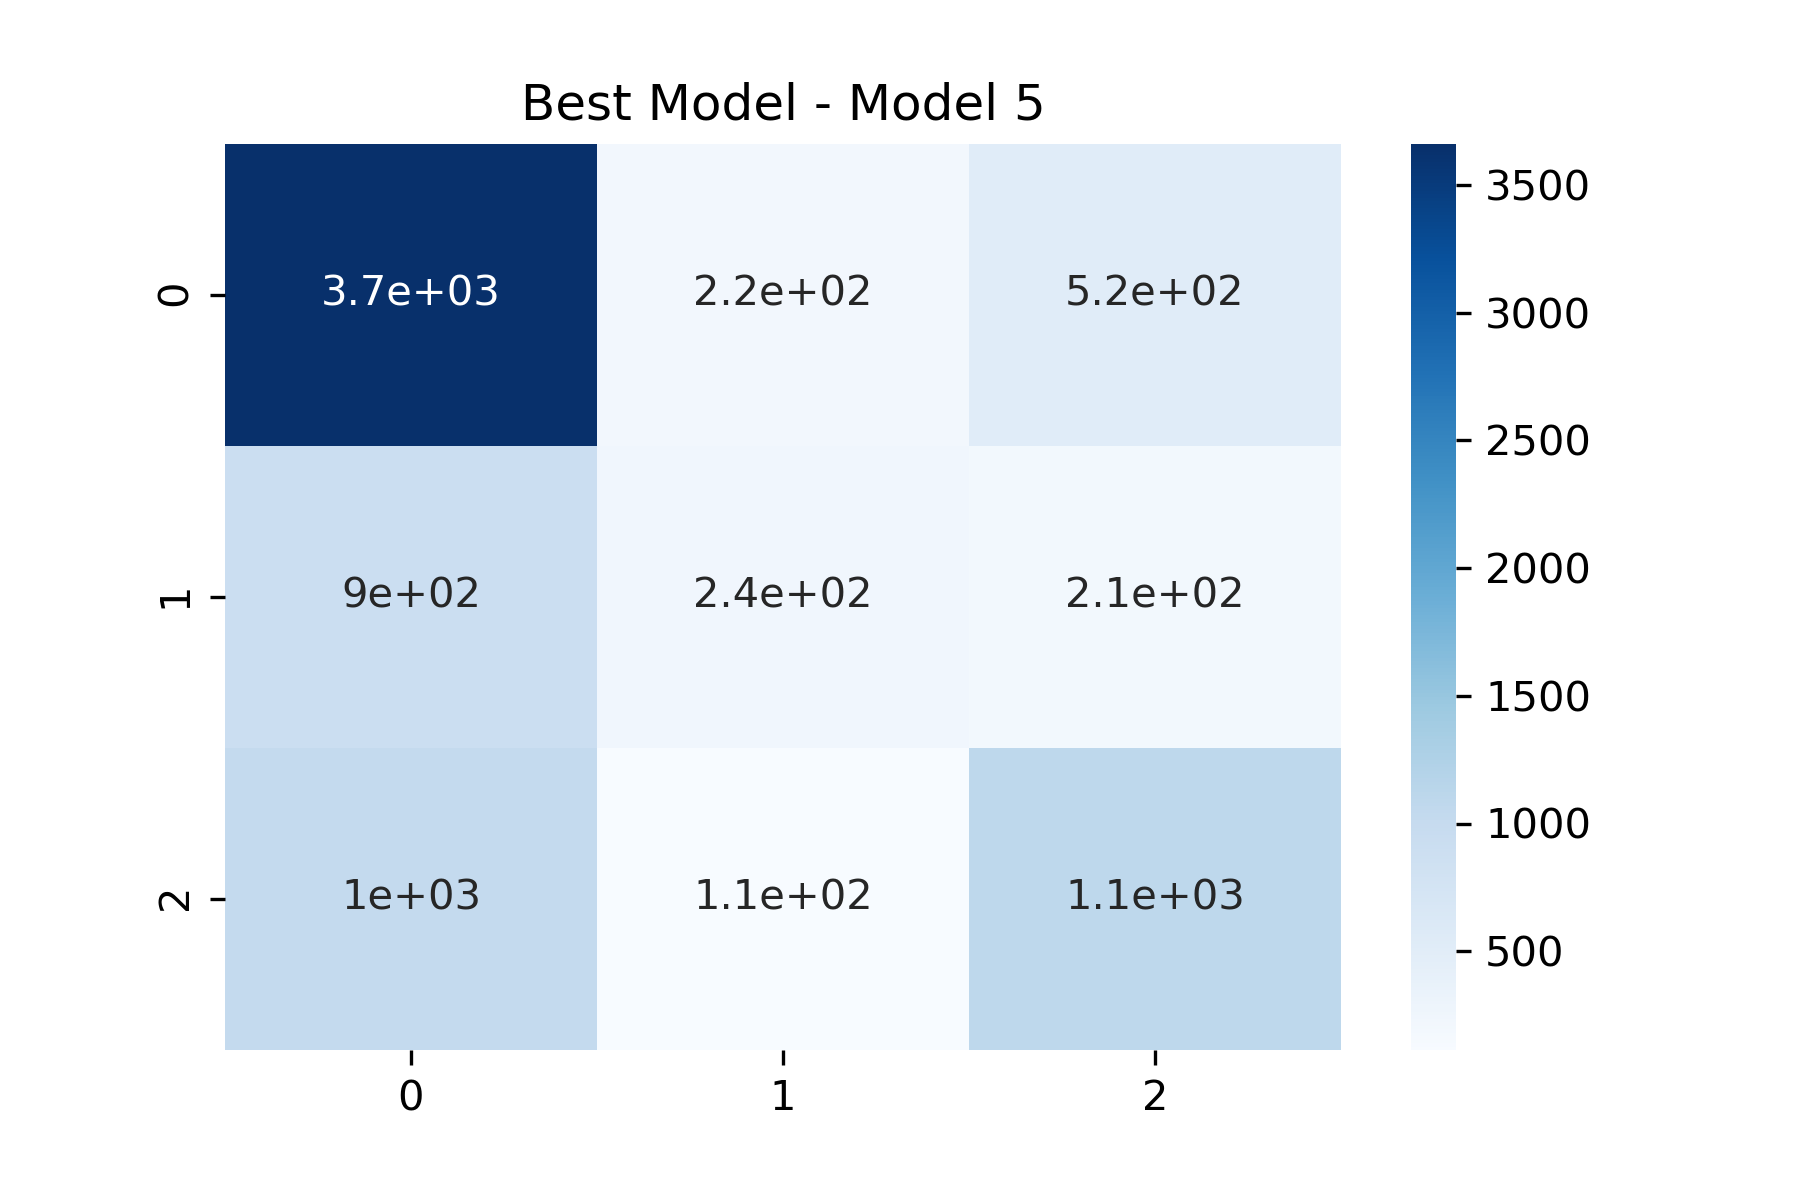
\includegraphics[scale=0.5]{figures/ns_m5cm}
    \label{fig:ns_m5cm}
}

\end{center}
\caption{Model 5 Results}
\label{fig:model5results}
\end{figure}

\newpage

\subsection{Results Discussion \& Final Model Selection}
Based on the results presented in the previous pages, it is evident that while the non-sampled dataset produces a higher accuracy in all models, the performance of the remaining evaluation metrics suffer due to the imbalance of classes within the dataset. The best accuracies for the non-sampled models are provided in Table \ref{tbl:best_acc_ns} 


\begin{table}[tbp]
\centering
\begin{tabularx}{\linewidth}{ l l X}
\toprule
   Model & Best Accuracy & Classifier \\
\midrule

Model 1 (5 Classes) & 0.604 & XGBoost Classifier and BOW \\
Model 2 (4 Classes) & 0.651 & XGBoost Classifier and BOW \\
Model 3 (4 Classes) & 0.602 & Random Forrest Classifier and TFIDF \\
Model 4 (3 Classes) & 0.686 & XGBoost Classifier and BOW \\ 
Model 5 (3 Classes) & 0.627 & Support Vector Machine Classifier and BOW \\

\bottomrule
\end{tabularx}
\caption{Best Accuracies for Non-sampled models}
\label{tbl:best_acc_ns}
\end{table}


 

Since \textit{class 0} is more abundant in the dataset and hence the training set, the model is biased towards accurately predicting it. However, as can be seen from the confusion matrices for each of the model results (in the non-sampled dataset), the model is unable to accurately predict the remainder of the classes very well. This poses as a great drawback of the model regardless of the high accuracy. 

Instead, it is a better choice to proceed with using a model within an under-sampled dataset. As can be seen from results – while it has poorer accuracy than its non-sampled counterpart, the remainder of the evaluation metrics appear to be higher in almost all cases. Additionally, the confusion matrix for the under-sampled dataset shows a higher variety of predictions made by the model. 

As for the final model which can be used to predict labels across a much larger / full dataset to feed into the dashboard, it is important to select the model with the highest (Macro) F1 Score. F1 Score is being considered as the main evaluation metrics in this case as we can see that relying solely on accuracy can be unwise (due to data biases), and furthermore that the F1 Score is a component of both Precision and Recall. As such, the results with the highest Macro F1 Scores using under-sampled data is shown in Table \ref{tbl:best_f1_us}


\begin{table}[tbp]
\centering
\begin{tabularx}{\linewidth}{ l l X}
\toprule
   Model & Best Macro F1 & Classifier \\
\midrule

Model 1 (5 Classes) & 0.429 & XGBoost Classifier and BOW \\
Model 2 (4 Classes) & 0.497 & XGBoost Classifier and BOW \\
Model 3 (4 Classes) & 0.502 & Logistic Regression Classifier and TFIDF \\
Model 4 (3 Classes) & 0.503 & Logistic Regression Classifier and TFIDF \\ 
Model 5 (3 Classes) & 0.532 & Logistic Regression Classifier and BOW\\

\bottomrule
\end{tabularx}
\caption{Best F1 Score for Under-sampled models}
\label{tbl:best_f1_us}
\end{table}

Additionally, since the objective of the project is to predict the vaccine related misinformation, Models 4 and 5 can be ruled out as these models only factor in three classes without the nuanced difference between the type of misinformation. These were presented solely to capture a what-if scenario. Similarly, Model 1 can be ruled out as five classes causes the performance of the model to be too poor (almost all evaluation metrics are below the 50\% threshold). This leaves only Models 2 and 3 – with the main difference being whether to remove class 4 entirely (as in Model 2) or merge it with class 1 (as with Model 3). 

Based on the model results presented earlier, the classifier which achieved the highest F1 Macro score (0.502) between Models 2 and 3 was Model 3’s Logistic Regression classifier, using TFIDF as a vectorizer and the following hyper-parameters: C = 1. 
Other metrics for this classifier are as follows:

\begin{itemize}
\item Accuracy: 0.504
\item Precision (Macro): 0.512
\item Recall (Macro): 0.504
\end {itemize}

While these metrics may not be impressive at first glance, it must be emphasized that these are with less than 5,000 training samples overall (see Table \ref{tbl:model1_details}  to Table \ref{tbl:model5_details} for exact breakdown). It is expected that with additional annotated data available – possibly doubling the current sampling per class, the metrics can improve significantly.
Finally, it must be noted that a significant content drift was observed for the Tweets from February 2020 to March 2020 as the normal conversation (as it relates to vaccines) began to shift from the usual vaccine related opinions and (mis)information to a conversation about a vaccine to tackles the COVID-19 Pandemic. The trends observed in the conversation included frustration and distrust towards pharmaceutical companies and political figures.  

\newpage

\section{Deriving Insights}
\textbf{Important Note: The metrics presented for this dashboard are deemed to be inaccurate and must not to be relied upon for decision support by Public Health Ontario or any other entity till such time that the model performance is improved with additional data annotation}
\subsection{Dashboard}
With the various machine learning models evaluated and the final one selected, the model can be applied to the overall dataset to make predictions for the vaccine related misinformation. For this project, an interactive dashboard was created in Tableau. The figure below shows a snapshot of this dashboard. 


The dashboard is comprised of five distinct components (referred to as sheets within Tableau). These are described in Table \ref{tbl:db_sheets} 

\begin{figure}[tbp]
\centering 
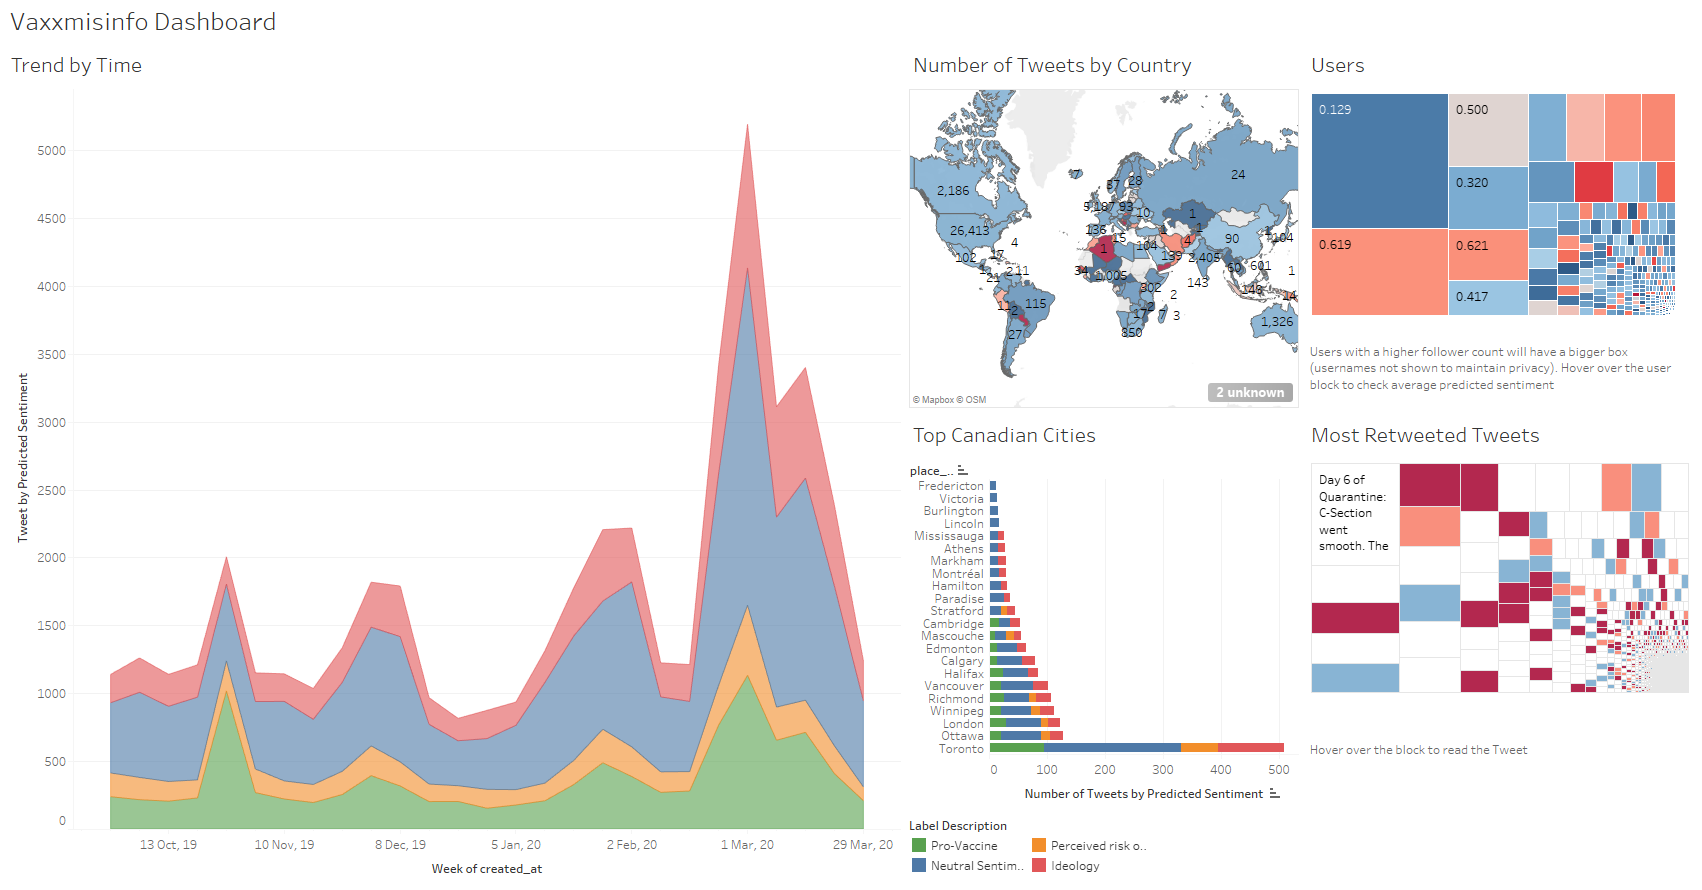
\includegraphics[width=1\textwidth]{figures/db_sample}
\caption{Dashboard sample} 
\label{fig:db_sample}
\end{figure}


\begin{table}[tbp]
\centering
\begin{tabularx}{\linewidth}{ l X}
\toprule
   Component / Sheet & Purpose \\
\midrule
Trend by time & This component shows the predicted label of the Tweet (and its web-scraped data) over time. The colour coding is based on the predicted label description \newline \\
Number of Tweets by Country & This shows the number of Tweets from a specific country. The colour with which the country is shaded is based on the average prediction of the Tweet’s vaccine misinformation, with red indicating higher degree of misinformation, blue indicating no misinformation and gray being in between.  \newline \\
Users & This shows the users with the highest follower count. To maintain privacy, the user details has been omitted from the dashboard. The Trend by time and the Number of Tweets by Country can be filtered by this component. 
Similar to above, the colour is indicative of the average misinformation by a particular user. \newline \\
Most Retweeted Tweets & The Tweets with the highest number of Re-Tweets. 
Similar to above, the colour is indicative of the average misinformation for the particular Tweet. \newline \\
Top Canadian Cities & The Canadian cities with the most Tweets, broken down by the predicted label. \newline \\


\bottomrule
\end{tabularx}
\caption{Dashboard components/sheets and their descriptions}
\label{tbl:db_sheets}
\end{table}

\newpage
\subsection{Global Calculated Fields}
Two new calculated columns were created within Tableau to assist in data manipulation and aggregation. These are described below along with the calculation. 

\paragraph{Pos/neg/Neut}
\begin{verbatim} 
IF
[y_pred] = 0 THEN 'Positive' 
ELSEIF
[y_pred] = 1 THEN 'Neutral' 
ELSEIF
[y_pred] = 2 THEN 'Negative' 
ELSEIF
[y_pred] = 3 THEN 'Negative' 
ELSEIF
[y_pred] = 4 THEN 'Neutral' 
END
\end{verbatim}

\paragraph{Label Description}

\begin{verbatim} 
IF
[y_pred] = 0 THEN 'Pro-Vaccine' 
ELSEIF
[y_pred] = 1 THEN 'Neutral Sentiment' 
ELSEIF
[y_pred] = 2 THEN 'Perceived risk or benefit of getting vaccinated' 
ELSEIF
[y_pred] = 3 THEN 'Ideology' 
ELSEIF
[y_pred] = 4 THEN 'Other' 
END

\end{verbatim}

\newpage
\subsection{Sheets Overview}
\paragraph{Sheet: Trend by time}
This sheet shows the predicted label of the Tweet over time. By default a weekly view is shown, however it can be drilled down to show a day-by-day trend, or rolled up to a monthly, quarterly or yearly trend. See Figure \ref{fig:trendbytime} for a sample.

\begin{figure}[tbp]
\begin{center}

\subfigure[\textit{Trend by time} sample]{
    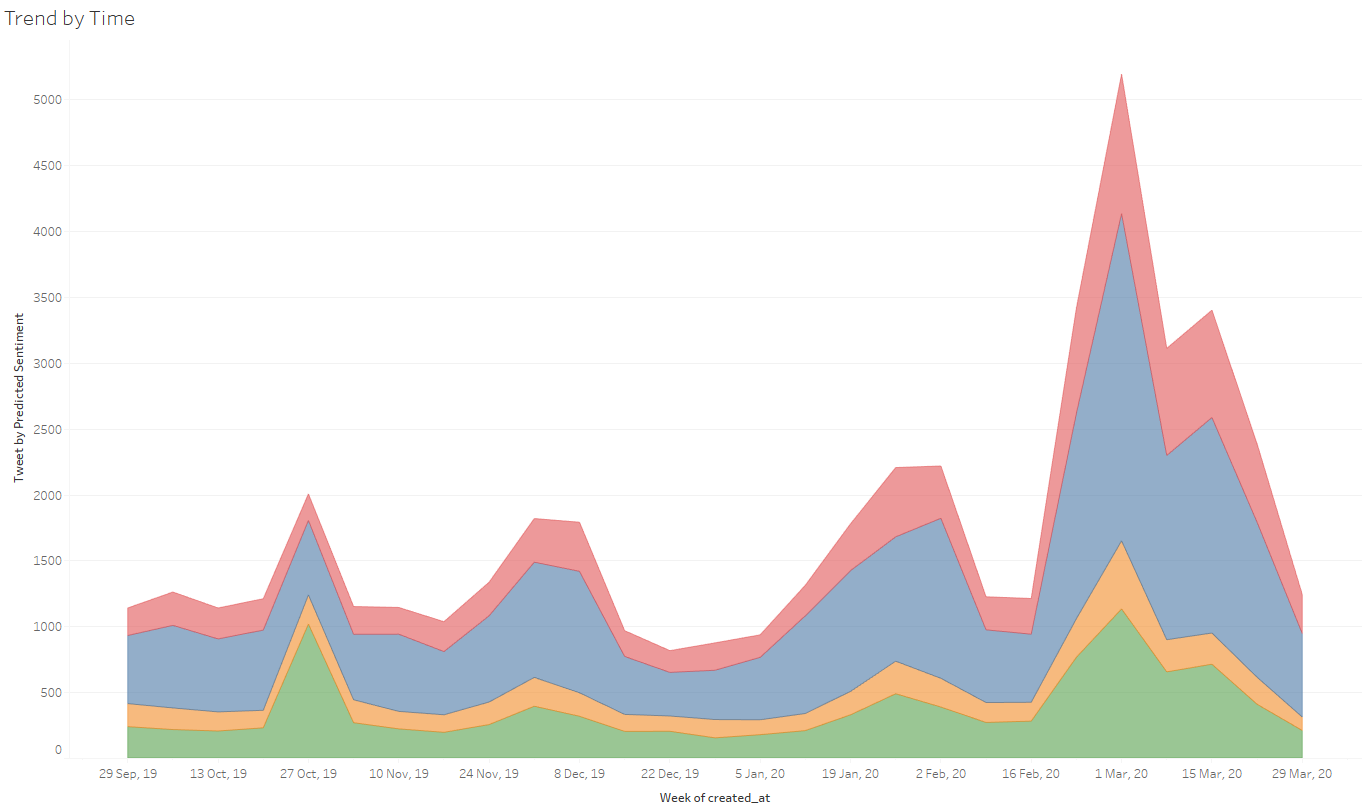
\includegraphics[scale=0.4]{figures/trendbytime}
    \label{fig:trendbytime}
}
\subfigure[Legend]{
    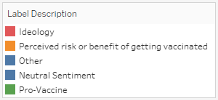
\includegraphics[scale=0.7]{figures/trendbytimelegend}
    \label{fig:trendbytimelegend}
}
\end{center}
\caption{Trend by time sample}
\label{fig:trendbytime}
\end{figure}


\paragraph{Sheet: Number of Tweets by Country}
This sheet shows the number of Tweets by Country available in the dataset. The colour is based on the ‘degree of misinformation’, with a blue shade indicating a lower degree of vaccine related misinformation and red shade indicating a higher degree of vaccine related misinformation. See Figure \ref{fig:country} for details.

\begin{figure}[tbp]
\centering 
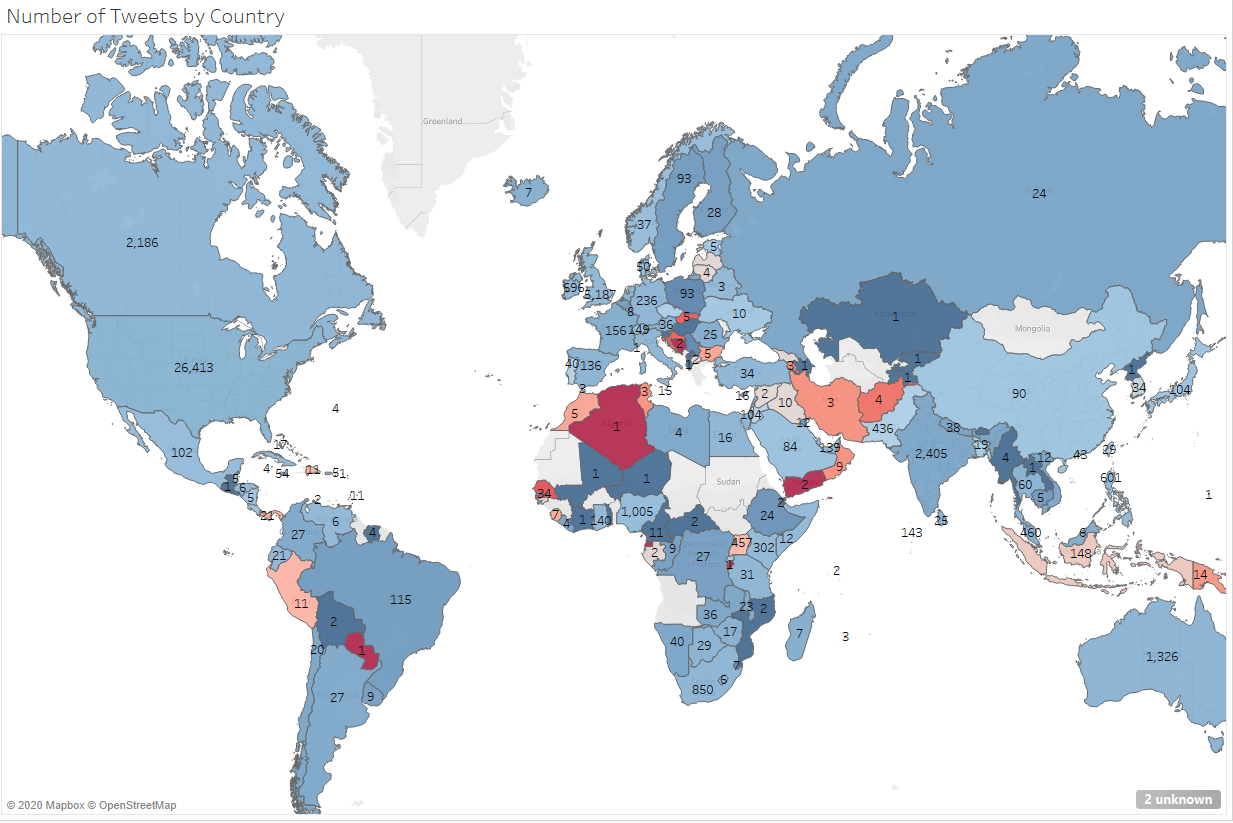
\includegraphics[width=0.8\textwidth]{figures/country}
\caption{\textit{Number of Tweets by Country} sample} 
\label{fig:country}
\end{figure}


\paragraph{Sheet: Users}
This sheet shows the Users (anonymized) with the highest follower counts. The size of the block indicates the number of followers a user has. The colour and the label within the block is based on the ‘degree of misinformation’, with a blue shade indicating a lower degree of vaccine related misinformation and red shade indicating a higher degree of vaccine related misinformation. See Figure \ref{fig:users} for a sample.

\begin{figure}[tbp]
\centering 
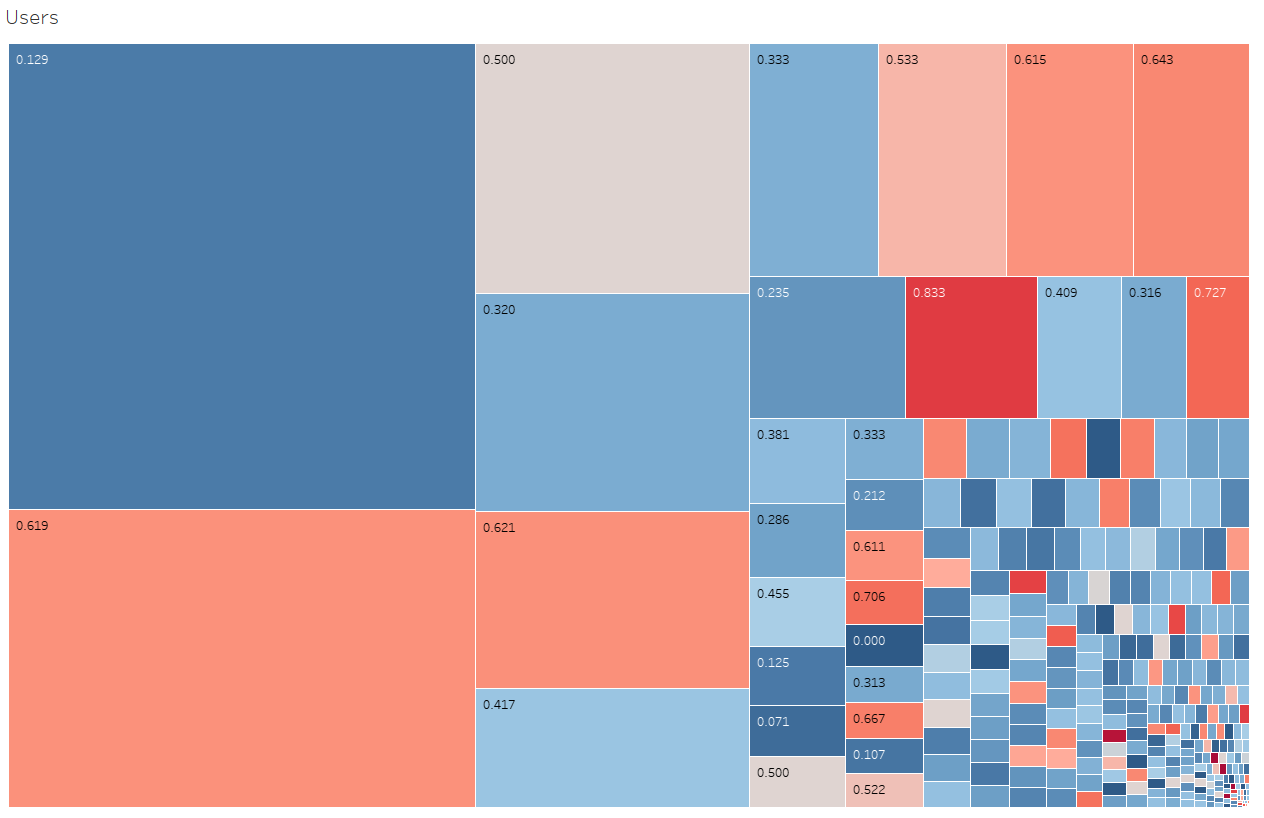
\includegraphics[width=0.8\textwidth]{figures/users}
\caption{\textit{Users} sample} 
\label{fig:users}
\end{figure}


\paragraph{Sheet: Most Retweeted Tweets}
This sheet shows the full text of the Tweet. The colour is based on the ‘degree of misinformation’, with a blue shade indicating a lower degree of vaccine related misinformation and red shade indicating a higher degree of vaccine related misinformation. See Figure \ref{fig:most_rt} for a sample.

\begin{figure}[tbp]
\centering 
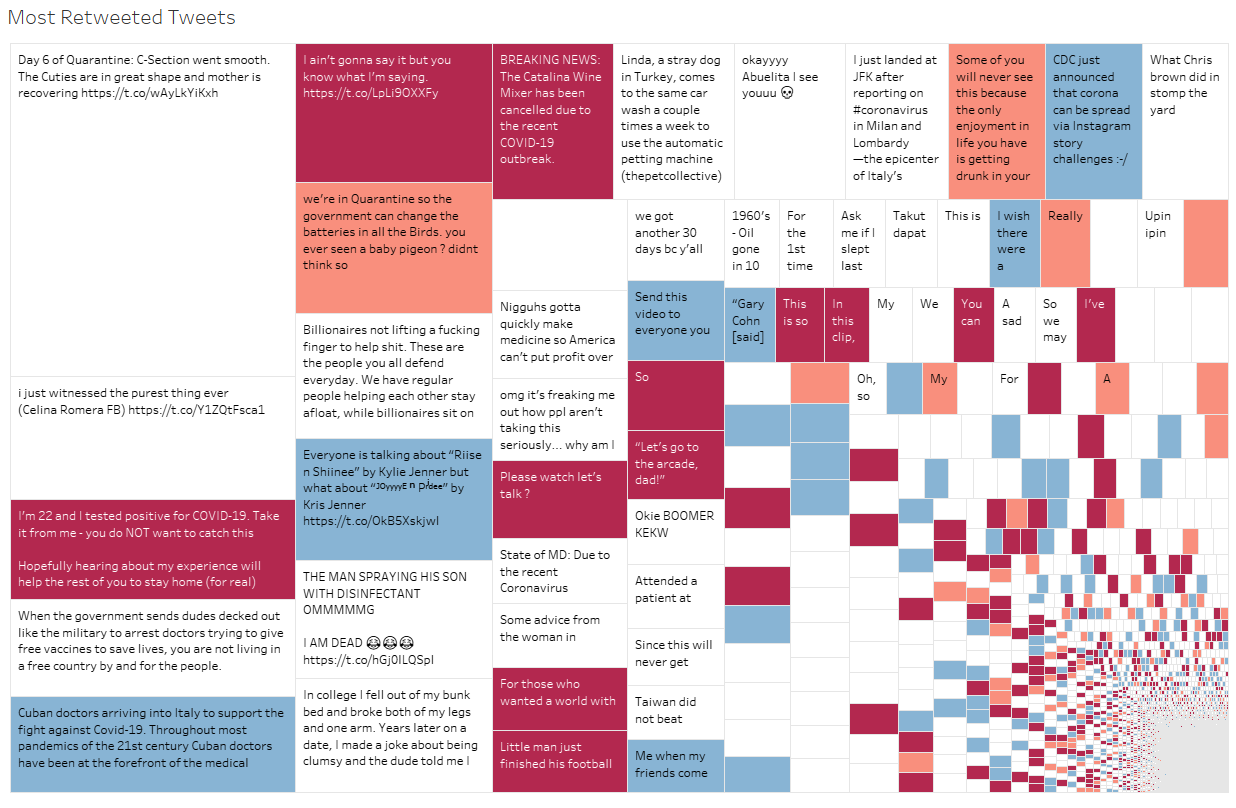
\includegraphics[width=0.8\textwidth]{figures/most_rt}
\caption{\textit{Most Retweeted Tweets} sample} 
\label{fig:most_rt}
\end{figure}

\paragraph{Sheet: Top Canadian Cities}
Since this Dashboard is intended to be focused on Canada, this sheet has been created to show the number of Tweets by predicted categories within Canadian cities. See Figure \ref{fig:topcan} for a sample.

\begin{figure}[tbp]
\centering 
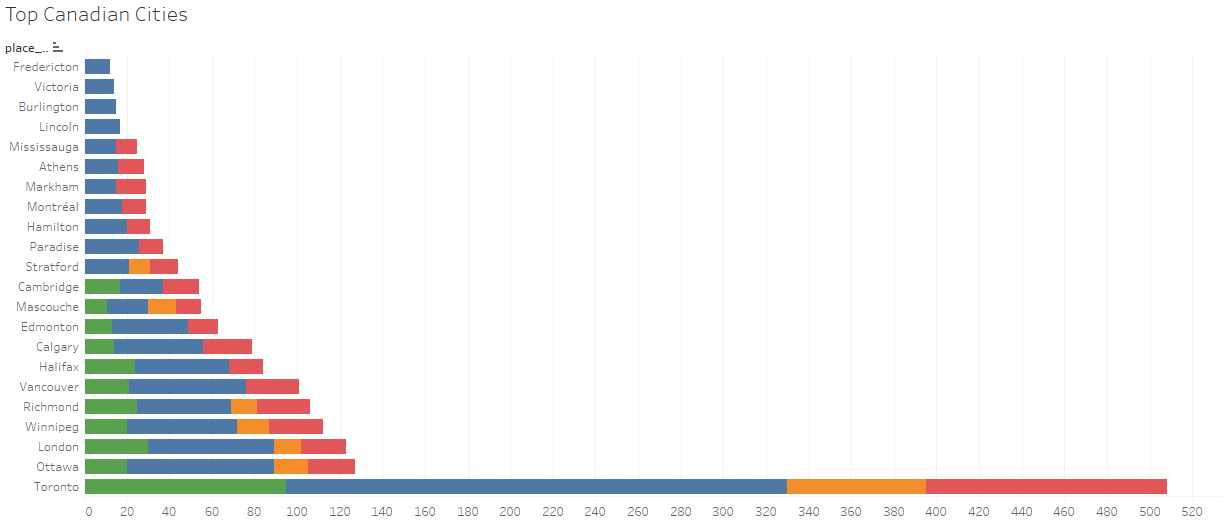
\includegraphics[width=1\textwidth]{figures/topcan}
\caption{\textit{Top Canadian Cities} sample} 
\label{fig:topcan}
\end{figure}

\subsection{Dashboard use cases}
The dashboard created in Tableau represents a visual way of analyzing any desired Key Performance Indicators (KPI’s) that researchers would like to see. One of the main use cases for the dashboard is to complement and potentially replace traditional survey methods on vaccine sentiment. \newline

A standard dashboard consists of multiple graphs and charts which ultimately affect the outcome of one another based on certain filters and selections applied. An example of this would be by selecting Canada in Figure \ref{fig:country}; the outcome of Figures \ref{fig:users} to \ref{fig:topcan}  would filter out any non-Canadian tweet (by location of tweet posted).

This organizational structure of displaying the data can be used by policy-makers to understand user rationale and ultimately make informed decisions.  For example, if a country is heavily spreading misinformation, the dashboards can be used to see which regions are antivax \textit{“hotspots”}.  Alternatively, researchers could use this information to identify trends in vaccine hesitancy over time, and also understand if there are any major differences and nuances between different geographies to understand the cause of hesitancy better.  As such, it is extremely critical to capture this information for the general health and well-being of people. \newline
Utilizing a dashboard which updates in real-time has a detrimental impact to the generality of public health surveillance.  Data is consistently being published publicly, which can carry meaningful information that could help make a difference for the future.  In the workflow, machine learning  is an efficient way to classify the information, while the dashboard can be used to display that information in real-time.

\newpage
\section{Conclusion \& Recommendations}
\paragraph{In conclusion} This project provides a strong framework for quickly training and deploying a machine learning model to detect vaccine related misinformation on social media. While the accuracy (and other metrics) evaluated within this project are not high enough to allow for it to be effectively used for decision support by Public Health agencies and local public health units, it is understood that there is high potential in its future use once the model can be made accurate enough (some recommendations provided below). This has the potential to be used as a tool for policy makers and public health officials to gain data driven insights and tackle one of the greatest threats to public health: misinformation. \newline


\paragraph{Several steps can be taken to further improve the machine learning model}

\paragraph{More data} The first and most important is to annotate additional data. Most machine learning models require thousands of training samples per class in-order to perform accurate enough to derive insights out of. As such, for the Dashboard to serve a greater value and serve to be more accurate, it would be highly recommended to gather and annotate additional data points. 


\paragraph{Dataset timeframe} Secondly, as a content drift was observed within the dataset, it is recommended to shift the timeframe of the dataset to end on December 2019. This is to allow for a dataset with Tweets (and conversations) with a COVID-19 related content mostly filtered out of the mainstream media and for the machine learning model to produce better results (as the content does not shift).  Additionally, with a short timeframe it is difficult to observe seasonality within the data – as such a recommendation would be to expand the timeframe of the tweets to be at-least 12 months, and possibly even 24 months. This would (hopefully) show the prevalence of a certain type of misinformation within a specific season / month. For example, a higher level of misinformation around flu season, or a spike in misinformation tied to a political event or a viral news/media.


\paragraph{Word embeddings and Neural Nets} Thirdly, some of the technical ways that can be explored are in implementing pre-trained word embeddings (such as GloVe, word2vec etc.). Word embedding methods learn a real-valued vector representation for a predefined fixed sized vocabulary from a corpus of text. Additionally, Neural Networks with custom NLP based architectures could be explored, specifically Recurrent Neural Networks (RNN) with Long Short-Term Memory (LSTM) networks which have shown to produce highly accurate results (given enough data - see \cite{jiang-2017} for relevant work) - and also the GPT3 model. Features beyond Natural Language can also be explored as inputs into the model training. These features can be location, number of followers, number of re-tweets etc. 

	
\paragraph{Faster annotation process} Fourthly, one of the biggest bottlenecks within this project was the time taken to annotate the labels (due to the higher quality and rigour of the annotation process). An idea that could be explored is to develop a simpler three class model (not misinformation, misinformation, neither) which would be highly accurate. Using this model to make predictions over the entire dataset, and then using these predictions as a guide to annotate further nuances within the type of misinformation. For example, with the predictions for misinformation, further annotating them to identify their specific types. Alternatively, the value of a simple three class model by itself can be explored paired with a strong Dashboard (as presented above).

\paragraph{Social network analysis} Fifthly, an idea that can be explored and incorporated is that of a social network analysis. This has been useful in identifying social "bubbles" or echo chambers \cite{cnet-2016, garimella-2017}. This can further allow Public Health units to observe territorial/provincial/regional variations of vaccine sentiment and misinformation. Similar concepts can be used to develop detectors of bots spreading misinformation, such as from work done by \cite{davis-2016}. 

\paragraph{Other datasets and languages} Finally, the dashboard created within this project was solely based on Twitter data. A future recommendation would be to pair this with News data over the same time period to overlay geo-political events, viral media and viral news to better provide insight into the root cause of the misinformation. The dataset used for this project was also limited to English Tweets, which leaves out a significant portion of the bi-lingual speaking (Canadian) population who may be Tweeting or using Social Media in French or other languages. A recommendation would be to implement this model for languages other than English as well.  

\newpage



\section{Appendix}

\begin{table}[h]
\centering
\begin{tabularx}{\linewidth}{ X X X X }
\toprule
\#hearus&FDA&poisoning&ugly truth\\
aborted tissue&fetal&population&VAERS\\
africa&fetal cells&population control&vaxxed\\
africa&fetus&profit&vaxxed\\
african&force&SIDS&victim\\
agenda&fraud&sterilization&victims\\
allergy&free choice&theft&wake up\\
aluminium&freedom&thimerosal&wakefield\\
aluminum&Gates&tissue&warfare\\
Bill&gilead&toxic&weapon\\
black&greed&kill&whistleblower\\
chip&hidden&liars&witnessed\\
choice&hoax&mandate&\\
compensation&injure&manmade&\\
control&injured&man-made&\\
corrupt&injuries&manufacture&\\
damage&injury&merck&\\
damage&insert&mercury&\\
diabetes&patent&monetize&\\
disclose&Poison&natural&\\
engineer&Patent&truth&\\


\bottomrule
\end{tabularx}
\caption{Negative Keywords}
\label{tbl:negkeywords}
\end{table}

\paragraph{Special Thanks}

to Justin Schonfeld of Public Health Agency of Canada for providing guidance throughout the project and Müller Martin Mathias from the Salathe Lab of Digital Epidemiology at the Swiss Federal Institute of Technology Lausanne (EPFL) for providing the dataset of Tweet IDs used for this project

\newpage
%\bibliographystyle{plain}
\bibliographystyle{ijocv081}
\bibliography{vaxxmisinfo_bib}

\end{document}